\section{Appendix}
\label{sec:appendix}

%\subsection{Dirichlet-based uncertainty models}
%
%In this section, we provide details on the losses used by each DBU model. \PostNetacro{}  uses a Bayesian loss which can be expressed as follows:
%
%\begin{equation}
%\begin{aligned}
%    L_{\mathrm{\PostNet}} &= \frac{1}{N} \sum_i \E_{q(p\dataix)}  [\mathrm{CE} (p\dataix, y\dataix)] - H(q\dataix)
%\end{aligned}
%\end{equation}
%where $\mathrm{CE}$ denotes the cross-entropy. Both the expectation term (i.e. $\E_{q(p\dataix)}  [\mathrm{CE} (p\dataix, y\dataix)]$) and the entropy term (i.e. $H(q\dataix)$) can be computed in closed-form \citep{charpentier2020}. \PriorNet uses a loss composed of two KL divergence terms for ID and OOD data: 
%\begin{equation}
%\begin{aligned}
%    L_{\mathrm{\PriorNet}} &= \frac{1}{N} \left[\sum_{\vx\dataix \in \text{ID data}}  [\mathrm{KL} [\mathrm{Dir} (\alpha^{\mathrm{ID}}) || q\dataix]]  \right. \\
%                           &+ \left.\sum_{\vx\dataix \in OOD data} [\mathrm{KL} [\mathrm{Dir} (\alpha^{\mathrm{OOD}}) || q\dataix]]\right]. \\
%\end{aligned}
%\end{equation}
%Both KL divergences terms can be computed in closed-form \citep{malinin2019}. The precision $\alpha^{\mathrm{ID}}$ and $\alpha^{\mathrm{OOD}}$ are hyper-parameters. The precision $\alpha^{\mathrm{ID}}$ is usually set to $1e^{1}$ for the correct class and $1$ otherwise. The precision $\alpha^{\mathrm{OOD}}$ is usually set to $\mathbf{1}$. \DDNet uses use the Dirichlet likelihood of soft labels produce by an ensemble of $M$ neural networks:
%\begin{equation}
%\begin{aligned}
%    L_{\mathrm{\DDNet}} &= - \frac{1}{N}  \sum_i \sum_{m=1}^{M} [\ln q\dataix(\pi^{im})] \\
%\end{aligned}
%\end{equation}
%where $\pi^{im}$ denotes the soft-label of $m$th neural network. The Dirichlet likelihood can be computed in closed-form \citep{malinin2019ensemble}. \EvNet uses the expected mean square error between the one-hot encoded label and the predicted categorical distribution:
%
%\begin{equation}
%\begin{aligned}
%    L_{\mathrm{\EvNet}} &= \frac{1}{N} \sum_i \E_{\vp\dataix \sim \text{Dir}(\bm{\alpha}\dataix)}||\vy*\dataix - \vp\dataix||^2 \\
%\end{aligned}
%\end{equation}
%where $\vy*\dataix$ denotes the one-hot encoded label. The expected MSE loss can also be computed in closed form \citep{sensoy2018}.
%For more details please have a look at the original paper on \PriorNet \citep{malini2018}, \PostNetacro{}  \citep{charpentier2020}, \DDNet \citep{malinin2019} and \EvNet \citep{sensoy2018}. 


\subsection{Closed-form computation of uncertainty measures \& Uncertainty attacks}
\label{subsec:appendix_measurecomp}

Dirichlet-based uncertainty models allow to compute several uncertainty measures in closed form (see \citep{malini2018} for a derivation). As proposed by \cite{malini2018}, we use precision~$m_{\alpha_0}$, differential entropy~$m_{\mathrm{diffE}}$ and mutual information~$m_{\mathrm{MI}}$ to estimate uncertainty on predictions.

The differential entropy $m_{\mathrm{diffE}}$ of a DBU model reaches its maximum value for equally probable categorical distributions and thus, a on flat Dirichlet distribution. It is a measure for distributional uncertainty and expected to be low on ID data, but high on OOD data. 
%
\begin{equation}
\begin{aligned}
	%m_{\mathrm{diffE}}  &= \sum_c^K \ln \Gamma (\alpha_c) - \ln \Gamma (\alpha_0) - \sum_c^K (\alpha_c -1) \cdot (\Psi (\alpha_c) - \Psi (\alpha_0))
	m_{\mathrm{diffE}}  = &\sum_c^K \ln \Gamma (\alpha_c) - \ln \Gamma (\alpha_0) \\
	&- \sum_c^K (\alpha_c -1) \cdot (\Psi (\alpha_c) - \Psi (\alpha_0))
\end{aligned}
\end{equation}
%
where $\alpha$ are the parameters of the Dirichlet-distribution, $\Gamma$ is the Gamma function and $\Psi$ is the Digamma function. 


The mutual information $m_{\mathrm{MI}}$ is the difference between the total uncertainty (entropy of the expected distribution) and the expected uncertainty on the data (expected entropy of the distribution). This uncertainty is expected to be low on ID data and high on OOD data. 
%
\begin{equation}
\begin{aligned}
	m_{\mathrm{MI}}  &= - \sum_{c=1}^{K} \frac{\alpha_c}{\alpha_0} \left( \ln \frac{\alpha_c}{\alpha_0} - \Psi(\alpha_c +1) + \Psi (\alpha_0 +1) \right)
\end{aligned}
\end{equation}

Furthermore, we use the precision~$\alpha_0$ to measure uncertainty, which is expected to be high on ID data and low on OOD data.
%
\begin{equation}
\begin{aligned}
	m_{\alpha_0}        &= \alpha_0 = \sum_{c=1}^{K} \alpha_c 
\end{aligned}
\end{equation}


As these uncertainty measures are computed in closed form and it is possible to obtain their gradients, we use them (i.e. $m_{\mathrm{diffE}}$, $m_{\mathrm{MI}}$, $m_{\alpha_0}$) are target function of our uncertainty attacks. Changing the attacked target function allows us to use a wide range of gradient-based attacks such as FGSM attacks, PGD attacks, but also more sophisticated attacks such as Carlini-Wagner attacks. 



\subsection{Details of the Experimental setup}
\label{subsec:exp_setup}

\textbf{Models.} We trained all models with a similar based architecture. We used namely 3 linear layers for vector data sets, 3 convolutional layers with size of 5 + 3 linear layers for MNIST and the VGG16 \cite{vgg} architecture with batch normalization for CIFAR10. All the implementation are performed using Pytorch \citep{pytorch}. We optimized all models using Adam optimizer. We performed early stopping by checking for loss improvement every 2 epochs and a patience of 10. The models were trained on GPUs (1 TB SSD).

We performed a grid-search for hyper-parameters for all models. The learning rate grid search was done in $[1e^{-5}, 1e^{-3}]$. For \PostNet, we used Radial Flows with a depth of 6 and a latent space equal to 6. Further, we performed a grid search for the regularizing factor in $[1e^{-7}, 1e^{-4}]$. For \PriorNet, we performed a grid search for the OOD loss weight in $[1, 10]$. For \DDNet, we distilled the knowledge of $5$ neural networks after a grid search in $[2, 5, 10, 20]$ neural networks. Note that it already implied a significant overhead at training compare to other models.

\textbf{Metrics.} For all experiments, we focused on using AUC-PR scores since it is well suited to imbalance tasks \citep{imbalance_apr} while bringing theoretically similar information than AUC-ROC scores \citep{apr_auroc}. We scaled all scores from $[0, 1]$ to $[0, 100]$. All results are average over 5 training runs using the best hyper-parameters found after the grid search.

\textbf{Data sets.} For vector data sets, we use 5 different random splits to train all models. We split the data in training, validation and test sets ($60\%$, $20\%$, $20\%$). 

We use the segment vector data set \cite{uci_datasets}, where the goal is to classify areas of images into $7$ classes (window, foliage, grass, brickface, path, cement, sky). We remove class window from ID training data to provide OOD training data to \PriorNet. Further, We remove the class 'sky' from training and instead use it as the OOD data set for OOD detection experiments. Each input is composed of $18$ attributes describing the image area. The data set contains $2,310$ samples in total.

We further use the Sensorless Drive vector data set \cite{uci_datasets}, where the goal is to classify extracted motor current measurements into $11$ different classes. We remove class 9 from ID training data to provide OOD training data to \PriorNet. We remove classes 10 and 11 from training and use them as the OOD dataset for OOD detection experiments. Each input is composed of $49$ attributes describing motor behaviour. The data set contains $58,509$ samples in total.

Additionally, we use the MNIST image data set \cite{mnist} where the goal is to classify pictures of hand-drawn digits into $10$ classes (from digit $0$ to digit $9$). Each input is composed of a $1 \times 28 \times 28$ tensor. The data set contains $70,000$ samples. For OOD detection experiments, we use FashionMNIST \cite{fashionmnist} and KMNIST \cite{kmnist} containing images of Japanese characters and images of clothes, respectively. FashionMNIST was used as training OOD for \PriorNet while KMNIST is used as OOD at test time.

Finally, we use the CIFAR10 image data set \cite{cifar10} where the goal is to classify a picture of objects into $10$ classes (airplane, automobile, bird, cat, deer, dog, frog, horse, ship, truck). Each input is a $3 \times 32 \times 32$ tensor. The data set contains $60,000$ samples. For OOD detection experiments, we use street view house numbers (SVHN) \cite{svhn}  and CIFAR100 \citep{cifar10} containing images of numbers and objects respectively. CIFAR100 was used as training OOD for \PriorNet while SVHN is used as OOD at test time.
 
\textbf{Perturbations.} For all label and uncertainty attacks, we used Fast Gradient Sign Methods and Project Gradient Descent. We tried 6 different attack radii $[0.0, 0.1, 0.2, 0.5, 1.0, 2.0, 4.0]$. These radii operate on the input space after data normalization. We bound perturbations by~$L_{\infty}$-norm or by~$L_2$-norm, with 
%
\begin{equation}
\begin{aligned}
	L_{\infty} (x) = \max_{i=1,\dots, D} \left|x_i\right| \mathrm{~~~~and~~~~}
	L_2 (x)        = (\sum_{i=1}^{D} x_i^2)^{0.5}.
\end{aligned}
\end{equation}
%
For $L_{\infty}$-norm it is obvious how to relate perturbation size~$\varepsilon$ with perturbed input images, because all inputs are standardized such that the values of their features are between~$0$ and~$1$.
A perturbation of size~$\varepsilon=0$ corresponds to the original input, while a perturbation of size~$\varepsilon=1$ corresponds to the whole input space and allows to change all features to any value. 

For~$L_2$-norm the relation between perturbation size~$\varepsilon$ and perturbed input images is less obvious. To justify our choice for~$\varepsilon$ w.r.t. this norm, we relate perturbations size~$\varepsilon_2$ corresponding to $L_2$-norm with perturbations size~$\varepsilon_{\infty}$ corresponding to $L_{\infty}$-norm. 
First, we compute~$\varepsilon_2$, such that the $L_2$-norm is the smallest super-set of the $L_{\infty}$-norm. Let us consider a perturbation of~$\varepsilon_{\infty}$. The largest~$L_2$-norm would be obtained if each feature is perturbed by~$\varepsilon_{\infty}$. Thus, perturbation~$\varepsilon_2$, such that $L_2$ encloses~$L_{\infty}$ is $\varepsilon_2 = (\sum_{i=1}^{D} \varepsilon_{\infty}^2)^{0.5} = \sqrt{D} \varepsilon_{\infty}$. For the MNIST-data set, with $D=28 \times 28$ input features $L_2$-norm with $\varepsilon_2=28$ encloses $L_{\infty}$-norm with~$\varepsilon_{\infty}=1$. 

Alternatively, $\varepsilon_2$ can be computes such that the volume spanned by~$L_2$-norm is equivalent to the one spanned by~$L_{\infty}$-norm. Using that the volume spanned by $L_{\infty}$-norm is $\varepsilon_{\infty}^D$ and the volume spanned by $L_2$-norm is 
$\frac{\pi^{0.5 D} \varepsilon_2^D}{\Gamma(0.5 D +1)}$ (where $\Gamma$ is the Gamma-function), we obtain volume equivalence if 
$\varepsilon_2 = \Gamma(0.5 D +1)^{\frac{1}{D}} \sqrt{\pi} \varepsilon_{\infty}$. For the MNIST-data set, with $D=28 \times 28$ input features $L_2$-norm with $\varepsilon_2 \approx 21.39$ is volume equivalent to $L_{\infty}$-norm with~$\varepsilon_{\infty}=1$.











\newpage 
\subsection{Additional Experiments}



Table~\ref{tab:acc_label_attack} and~\ref{tab:acc_label_attack_fgsm} illustrate that no DBU model maintains high accuracy under gradient-based label attacks. Accuracy under PGD attacks decreases more than under FGSM attacks, since PGD is stronger.  Interestingly Noise attacks achieve also good performances with increasing Noise standard deviation. Note that the attack is not constraint to be with a given radius for Noise attacks.



\begin{table*}[htbp!]
 	\centering
 	\caption{Accuracy under PGD label attacks.}
 	\begin{small}
		\resizebox{\textwidth}{!}{
 		\begin{tabular}{@{}rrrrrrrrc|crrrrrrr@{}}
 			\toprule
  			Att. Rad. & 0.0 & 0.1 & 0.2 & 0.5 & 1.0 & 2.0 & 4.0 & & & 0.0 & 0.1 & 0.2 & 0.5 & 1.0 & 2.0 & 4.0 \\
 			\midrule
 			& \multicolumn{7}{c}{MNIST} & & & \multicolumn{7}{c}{CIFAR10} \\
 			\PostNetacro{}   &  \textbf{99.4} &  \textbf{99.2} &  \textbf{98.8} &  96.8 &  89.6 &  53.8 &  13.0 & &
 			          &  89.5 &  73.5 &  51.7 &  13.2 &   2.2 &   0.8 &  0.3 \\
 			\PriorNet &  99.3 &  99.1 &  \textbf{98.8} &  97.4 &  \textbf{93.9} &  \textbf{75.3} &   4.8 & &
 			          &  88.2 &  \textbf{77.8} &  \textbf{68.4} &  \textbf{54.0} &  \textbf{37.9} &  \textbf{17.5} &  \textbf{5.1} \\
 		    \DDNet    &  \textbf{99.4} &  99.1 &  \textbf{98.8} &  \textbf{97.5} &  91.6 &  48.8 &   0.2 & &
 		              &  86.1 &  73.9 &  59.1 &  20.5 &   1.5 &   0.0 &  0.0 \\
 		    \EvNet    &  99.2 &  98.9 &  98.4 &  96.8 &  92.4 &  73.1 &  \textbf{40.9} & &
 		              &  \textbf{89.8} &  71.7 &  48.8 &  11.5 &   2.7 &   1.5 &  0.4 \\
 		    \midrule
 		 & \multicolumn{7}{c}{Sensorless} & & & \multicolumn{7}{c}{Segment} \\
 			\PostNetacro{}   &  98.3 &  13.1 &   6.4 &   4.0 &  \textbf{7.0} &  \textbf{9.8} &  \textbf{11.3} & &
 			          &  98.9 &  82.8 &  \textbf{50.1} &  \textbf{19.2} &  \textbf{8.8} &  \textbf{5.1} &  \textbf{8.6}   \\
 			\PriorNet &  \textbf{99.3} &  16.5 &   5.6 &   1.2 &  0.4 &  0.2 &   1.6 & &
 			          &  \textbf{99.5} &  90.7 &  47.6 &   7.8 &  0.2 &  0.0 &  0.4 \\
 		    \DDNet    &  \textbf{99.3} &  12.4 &   2.4 &   0.6 &  0.3 &  0.1 &   0.1 & &
 		              &  99.2 &  \textbf{90.8} &  45.7 &   6.9 &  0.0 &  0.0 &  0.0 \\
 		    \EvNet    &  99.0 &  \textbf{35.3} &  \textbf{22.3} &  \textbf{11.2} &  \textbf{7.0} &  5.2 &   4.0 & &
 		              &  99.3 &  91.8 &  54.0 &  10.3 &  0.8 &  0.5 &  0.6 \\
 			\bottomrule
 		\end{tabular}
		}
 	\end{small}
 	\label{tab:acc_label_attack}
\end{table*}



\begin{table*}[htbp!]
 	\centering
 	\caption{Accuracy under FGSM label attacks.}
 	\begin{small}
		\resizebox{\textwidth}{!}{
 		\begin{tabular}{@{}rrrrrrrrc|crrrrrrr@{}}
 			\toprule
 			Att. Rad. & 0.0 & 0.1 & 0.2 & 0.5 & 1.0 & 2.0 & 4.0 & & & 0.0 & 0.1 & 0.2 & 0.5 & 1.0 & 2.0 & 4.0 \\
 			\midrule
 			& \multicolumn{7}{c}{MNIST} & & & \multicolumn{7}{c}{CIFAR10} \\
 			\PostNetacro{}   & \textbf{99.4} &  \textbf{99.2} &  \textbf{98.9} &  97.7 &  95.2 &  \textbf{90.1} &  \textbf{79.2} & &
 			          & 89.5 &  72.3 &  54.9 &  31.2 &  21.0 &  16.8 &  15.6 \\
 			\PriorNet & 99.3 &  99.1 &  \textbf{98.9} &  97.7 &  \textbf{95.8} &  93.2 &  76.7 & &
 			          & 88.2 &  \textbf{77.3} &  \textbf{70.1} &  \textbf{59.4} &  \textbf{52.3} &  \textbf{48.5} &  \textbf{46.8} \\
 		    \DDNet    & \textbf{99.4} &  \textbf{99.2} &  \textbf{98.9} &  \textbf{97.8} &  94.7 &  79.2 &  25.2 & &
 			          & 86.1 &  73.0 &  60.2 &  32.5 &  14.6 &   7.1 &   6.0 \\
 		    \EvNet    & 99.2 &  98.9 &  98.6 &  97.6 &  \textbf{95.8} &  \textbf{90.1} &  74.4 & &
 			          & \textbf{89.8} &  71.4 &  54.5 &  29.6 &  18.1 &  14.4 &  13.4 \\
 		    \midrule
 		     & \multicolumn{7}{c}{Sensorless} & & & \multicolumn{7}{c}{Segment} \\
 			\PostNetacro{}   & 98.3 &  19.6 &  10.9 &  10.9 &  11.9 &  12.4 &  12.5 & &
 			          & 98.9 &  79.6 &  \textbf{57.3} &  \textbf{31.5} &  \textbf{18.4} &  \textbf{20.6} &  \textbf{19.9} \\
 			\PriorNet & \textbf{99.3} &  24.7 &  11.8 &   8.6 &   8.5 &   8.1 &   8.3 & &
 			          & \textbf{99.5} &  85.5 &  40.5 &   8.9 &   0.4 &   0.3 &   0.2 \\
 		    \DDNet    & \textbf{99.3} &  18.0 &   8.2 &   6.5 &   5.4 &   6.7 &   7.8 & &
 			          & 99.2 &  86.4 &  36.2 &  11.9 &   0.9 &   0.0 &   0.0 \\
 		    \EvNet    & 99.0 &  \textbf{42.0} &  \textbf{28.0} &  \textbf{17.5} &  \textbf{13.7} &  \textbf{13.6} &  \textbf{14.9} & &
 			          & 99.3 &  \textbf{90.6} &  55.2 &  14.2 &   2.4 &   0.5 &   0.1 \\
 			\bottomrule
 		\end{tabular}
		}
 	\end{small}
 	\label{tab:acc_label_attack_fgsm}
\end{table*}


\begin{table*}[htbp!]
 	\centering
 	\caption{Accuracy under Noise label attacks.}
 	\begin{small}
		\resizebox{\textwidth}{!}{
 		\begin{tabular}{@{}rrrrrrrrc|crrrrrrr@{}}
 			\toprule
 			%& \multicolumn{7}{c}{MNIST} & & & \multicolumn{7}{c}{CIFAR10} \\
 			%\cmidrule{2-8}  \cmidrule{11-16}
 			Noise Std & 0.0 & 0.1 & 0.2 & 0.5 & 1.0 & 2.0 & 4.0 & & & 0.0 & 0.1 & 0.2 & 0.5 & 1.0 & 2.0 & 4.0 \\
 			\midrule
 			& \multicolumn{7}{c}{MNIST} & & & \multicolumn{7}{c}{CIFAR10} \\
 			\PostNetacro{}   & \textbf{99.4} &  \textbf{98.6} &  91.8 &  \textbf{14.9} &  \textbf{1.3} &  \textbf{0.1} &  0.0 & &
 			          & \textbf{91.7} &  21.5 &  10.1 &   0.1 &   1.2 &  0.0 &  1.9 \\
 			\PriorNet & 99.3 &  98.5 &  \textbf{95.7} &  14.4 &  0.0 &  0.0 &  0.0 & &
 			          & 87.7 &  \textbf{28.1} &  \textbf{11.2} &   9.7 &   5.0 &  \textbf{8.5} &  \textbf{9.0}\\
 		    \DDNet    & \textbf{99.4} &  \textbf{98.6} &  92.4 &  13.3 &  0.7 &  0.0 &  0.0 & &
 			          & 81.7 &  23.0 &  \textbf{11.2} &  \textbf{11.2} &  \textbf{11.0} &  7.8 &  6.7 \\
 		    \EvNet    & 99.3 &  96.9 &  81.6 &  11.7 &  0.5 &  0.0 &  0.0 & &
 			          & 89.5 &  20.7 &  11.1 &   5.2 &   0.5 &  2.3 &  3.9 \\
 		    \midrule
 		     & \multicolumn{7}{c}{Sensorless} & & & \multicolumn{7}{c}{Segment} \\
 			\PostNetacro{}   & 98.1 &  0.1 &  \textbf{3.7} &  \textbf{11.7} &  \textbf{11.7} &  \textbf{11.7} &  \textbf{11.7} & &
 			          & 98.5 &  39.4 &   3.9 &  \textbf{1.8} &  \textbf{12.1} &  \textbf{20.3} &  \textbf{22.1} \\
 			\PriorNet & \textbf{99.3} &  0.2 &  0.0 &   0.0 &   0.0 &   0.3 &   2.4 & &
 			          & \textbf{99.4} &  47.9 &   8.8 &  0.0 &   0.0 &   0.0 &   0.0 \\
 		    \DDNet    & 99.0 &  \textbf{0.4} &  0.1 &   0.0 &   0.0 &   0.0 &   0.0 & &
 			          & 99.1 &  50.0 &  \textbf{10.3} &  0.0 &   0.0 &   0.3 &   0.0 \\
 		    \EvNet    & 98.6 &  0.2 &  0.0 &   0.1 &   1.4 &   4.6 &   8.8 & &
 			          & 99.1 &  \textbf{50.3} &  \textbf{10.3} &  1.2 &   0.3 &   0.0 &   1.5 \\
 			\bottomrule
 		\end{tabular}
		}
 	\end{small}
 	\label{tab:acc_label_attack_noise_attack}
\end{table*}

\clearpage
\subsubsection{Uncertainty estimation under label attacks}

\textbf{Is low uncertainty a reliable indicator of correct predictions?}

On non-perturbed data uncertainty estimates are an indicator of correctly classified samples, but if the input data is perturbed none of the DBU models maintains its high performance. Thus, uncertainty estimates are not a robust indicator of correctly labeled inputs. 

\begin{table*}[htbp!]
 	\centering
 	\caption{Distinguishing between correctly and wrongly predicted labels based on the differential entropy under PGD label attacks (AUC-PR).}
 	\begin{small}
		\resizebox{\textwidth}{!}{
 		\begin{tabular}{@{}rrrrrrrrc|crrrrrrr@{}}
 			\toprule
 			& \multicolumn{7}{c}{MNIST} & & & \multicolumn{7}{c}{Segment} \\
 			\cmidrule{2-8}  \cmidrule{11-17}
 			Att. Rad. & 0.0 & 0.1 & 0.2 & 0.5 & 1.0 & 2.0 & 4.0 & & & 0.0 & 0.1 & 0.2 & 0.5 & 1.0 & 2.0 & 4.0 \\
 			\midrule
 			%& \multicolumn{7}{c}{MNIST} & & & \multicolumn{7}{c}{Segment} \\
 			\PostNetacro{}   &  99.9 &   99.9 &  99.8 &  98.7 &  89.5 &  43.5 &   9.0 & & 
 			          &  99.9 &  77.6 &  31.6 &  \textbf{11.1} &  \textbf{5.3} &  \textbf{4.4} &   8.7 \\
 			\PriorNet &  99.9 &   99.8 &  99.6 &  97.7 &  90.5 &  \textbf{69.1} &   6.4 & & 
 			          &  \textbf{100.0} &  \textbf{96.8} &  44.5 &   4.5 &  0.4 &  0.0 &  \textbf{15.2} \\
 		    \DDNet    &  \textbf{100.0} &  \textbf{100.0} &  \textbf{99.9} &  \textbf{99.7} &  \textbf{97.6} &  50.2 &   0.1 & &
 		              &  \textbf{100.0} &  \textbf{96.8} &  \textbf{54.0} &   4.3 &  0.0 &  0.0 &   0.0 \\
 		    \EvNet    &  99.6 &   99.3 &  98.7 &  96.1 &  88.8 &  63.1 &  \textbf{31.7} & &
 		              &  \textbf{100.0} &  95.9 &  44.3 &   5.9 &  0.8 &  0.6 &   0.7 \\
 			\bottomrule
 		\end{tabular}
		}
 	\end{small}
 	\label{tab:conf_label_attack_2}
\end{table*}



\begin{table*}[htbp!]
 	\centering
 	\caption{Distinguishing between correctly and wrongly predicted labels based on the precision~$\alpha_0$ under PGD label attacks (AUC-PR).}
 	\begin{small}
		\resizebox{\textwidth}{!}{
 		\begin{tabular}{@{}rrrrrrrrc|crrrrrrr@{}}
 			\toprule
 			%& \multicolumn{7}{c}{MNIST} & & & \multicolumn{7}{c}{CIFAR10} \\
 			%\cmidrule{2-8}  \cmidrule{11-16}
 			Att. Rad. & 0.0 & 0.1 & 0.2 & 0.5 & 1.0 & 2.0 & 4.0 & & & 0.0 & 0.1 & 0.2 & 0.5 & 1.0 & 2.0 & 4.0 \\
 			\midrule
 			& \multicolumn{7}{c}{MNIST} & & & \multicolumn{7}{c}{CIFAR10} \\
            \PostNetacro{}   & \textbf{100.0} &   99.9 &   99.7 &  98.2 &  87.9 &  39.1 &   6.9 & &
                      & \textbf{98.7} &  88.6 &  56.2 &   7.8 &   1.2 &   0.4 &  0.3  \\
            \PriorNet &  99.9 &   99.8 &   99.6 &  97.7 &  90.4 & \textbf{69.1} &   6.6  & &
                      &  92.9 &  77.7 &  60.5 & \textbf{37.6} & \textbf{24.9} & \textbf{11.3} & \textbf{3.0} \\
            \DDNet    & \textbf{100.0} & \textbf{100.0} & \textbf{100.0} & \textbf{99.8} & \textbf{98.2} &  51.1 &   0.1  & &
                      &  97.6 & \textbf{91.8} & \textbf{78.3} &  18.1 &   0.8 &   0.0 &  0.0  \\
            \EvNet    &  99.6 &   99.2 &   98.6 &  95.7 &  88.6 &  63.6 & \textbf{32.6} & &
                                  &  97.9 &  85.9 &  57.2 &  10.2 &   4.0 &   2.4 &  0.3  \\
 		    \midrule
 		     & \multicolumn{7}{c}{Sensorless} & & & \multicolumn{7}{c}{Segment} \\
            \PostNetacro{}   &  99.6 &   7.0 &   3.3 &  3.1 & \textbf{6.9} & \textbf{9.8} & \textbf{11.3} & &
                      &  99.9 &  74.2 &  31.6 & \textbf{11.1} & \textbf{5.0} & \textbf{4.2} & \textbf{8.6} \\
            \PriorNet &  99.8 &  10.5 &   3.2 &  0.6 &  0.2 &  0.2 &   1.8 & &
                     & \textbf{100.0} &  96.9 & \textbf{45.2} &   4.4 &  0.4 &  0.0 &  1.2  \\
            \DDNet    &  99.8 &   8.7 &   1.3 &  0.3 &  0.2 &  0.1 &   0.2 & &
                    & \textbf{100.0} & \textbf{97.1} &  45.0 &   4.1 &  0.0 &  0.0 &  0.0 \\
            \EvNet    & \textbf{99.9} & \textbf{23.2} & \textbf{13.2} & \textbf{6.0} &  3.7 &  2.7 &   2.1 & &
                    & \textbf{100.0} &  95.7 &  44.5 &   5.9 &  0.8 &  0.6 &  0.7 \\
 			\bottomrule
 		\end{tabular}
		}
 	\end{small}
 	\label{tab:conf_label_attack_alpha}
\end{table*}



\begin{table*}[htbp!]
 	\centering
 	\caption{Distinguishing between correctly and wrongly predicted labels based on the mutual information under PGD label attacks (AUC-PR).}
 	\begin{small}
		\resizebox{\textwidth}{!}{
 		\begin{tabular}{@{}rrrrrrrrc|crrrrrrr@{}}
 			\toprule
 			%& \multicolumn{7}{c}{MNIST} & & & \multicolumn{7}{c}{CIFAR10} \\
 			%\cmidrule{2-8}  \cmidrule{11-16}
 			Att. Rad. & 0.0 & 0.1 & 0.2 & 0.5 & 1.0 & 2.0 & 4.0 & & & 0.0 & 0.1 & 0.2 & 0.5 & 1.0 & 2.0 & 4.0 \\
 			\midrule
 			& \multicolumn{7}{c}{MNIST} & & & \multicolumn{7}{c}{CIFAR10} \\
            \PostNetacro{}   & 99.7 &  99.7 &  99.6 &  99.2 &  92.4 &  40.0 &   6.9 & &
                      & \textbf{97.3} &  84.5 &  56.2 &  12.2 &   2.4 &   0.7 &  0.3  \\
            \PriorNet &  99.9 &  99.8 &  99.6 &  97.7 &  90.3 & \textbf{68.9} &   6.4  & &
                      &  82.7 &  65.6 &  51.4 & \textbf{35.5} & \textbf{24.4} & \textbf{11.0} & \textbf{2.9} \\
            \DDNet    & \textbf{100.0} & \textbf{99.9} & \textbf{99.9} & \textbf{99.7} & \textbf{97.4} &  50.2 &   0.1  & &
                      &  96.9 & \textbf{90.8} & \textbf{77.2} &  18.8 &   0.8 &   0.0 &  0.0  \\
            \EvNet    &  97.8 &  97.0 &  95.7 &  92.6 &  86.1 &  62.3 & \textbf{28.9} & &
                      &  91.3 &  72.4 &  47.9 &  11.4 &   1.6 &   0.9 &  1.6  \\
 		    \midrule
 		     & \multicolumn{7}{c}{Sensorless} & & & \multicolumn{7}{c}{Segment} \\
            \PostNetacro{}   &  99.3 &   7.0 &   3.3 &  3.3 & \textbf{7.0} & \textbf{9.8} &  11.3 & &
                      &  99.9 &  73.2 &  31.5 & \textbf{11.1} & \textbf{5.0} & \textbf{4.3} & \textbf{8.7} \\
            \PriorNet & \textbf{99.8} &  10.5 &   3.2 &  0.6 &  0.2 &  0.1 & \textbf{11.8} & &
                      & \textbf{100.0} & \textbf{96.6} & \textbf{45.2} &   4.5 &  0.4 &  0.0 &  1.1  \\
            \DDNet    &  99.6 &   8.6 &   1.3 &  0.3 &  0.2 &  0.1 &   0.1 & &
                      & \textbf{100.0} &  96.5 &  42.4 &   4.1 &  0.0 &  0.0 &  0.0 \\
            \EvNet    &  99.1 & \textbf{22.0} & \textbf{12.6} & \textbf{5.9} &  3.7 &  2.7 &   2.2 & &
                      & \textbf{100.0} &  90.5 &  41.0 &   5.9 &  0.8 &  0.6 &  0.7 \\
 			\bottomrule
 		\end{tabular}
		}
 	\end{small}
 	\label{tab:conf_label_attack_mi}
\end{table*}


\begin{table*}[htbp!]
 	\centering
 	\caption{Distinguishing between correctly and wrongly predicted labels based on the differential entropy under FGSM label attacks (AUC-PR).}
 	\begin{small}
		\resizebox{\textwidth}{!}{
 		\begin{tabular}{@{}rrrrrrrrc|crrrrrrr@{}}
 			\toprule
 			%& \multicolumn{7}{c}{MNIST} & & & \multicolumn{7}{c}{CIFAR10} \\
 			%\cmidrule{2-8}  \cmidrule{11-16}
 			Att. Rad. & 0.0 & 0.1 & 0.2 & 0.5 & 1.0 & 2.0 & 4.0 & & & 0.0 & 0.1 & 0.2 & 0.5 & 1.0 & 2.0 & 4.0 \\
 			\midrule
 			& \multicolumn{7}{c}{MNIST} & & & \multicolumn{7}{c}{CIFAR10} \\
             \PostNetacro{}   & 99.9 &   99.9 &  99.8 &  99.4 &  97.8 & \textbf{92.1} & \textbf{83.2} & &
                      & \textbf{98.5} &  88.7 &  68.9 &  31.0 &  18.6 &  15.5 &  16.7 \\
            \PriorNet & 99.9 &   99.9 &  99.7 &  98.3 &  94.1 &  88.5 &  78.6  & &
                      & 90.1 &  73.6 &  61.6 & \textbf{46.1} & \textbf{38.5} & \textbf{35.6} & \textbf{37.3} \\
            \DDNet    & \textbf{100.0} & \textbf{100.0} & \textbf{99.9} & \textbf{99.8} & \textbf{98.7} &  86.4 &  23.0 & &
                      & 97.3 & \textbf{90.6} & \textbf{78.7} &  39.4 &  13.7 &   6.0 &   5.1 \\
            \EvNet    & 99.6 &   99.4 &  99.1 &  97.8 &  95.8 &  90.4 &  76.8 & &
                      & 98.0 &  86.2 &  67.4 &  32.7 &  19.9 &  18.2 &  19.7 \\		
 		    \midrule
 		     & \multicolumn{7}{c}{Sensorless} & & & \multicolumn{7}{c}{Segment} \\
             \PostNetacro{}   & 99.7 &  11.7 &   7.3 &   9.3 &  11.8 &  12.5 &  12.5 & &
                      & 99.9 &  73.6 &  40.6 & \textbf{23.7} & \textbf{17.2} & \textbf{19.8} & \textbf{20.2} \\
            \PriorNet & 99.8 &  21.4 &  10.4 &   8.5 &   9.0 &   9.2 &  10.3 & &
                      & \textbf{100.0} &  93.7 &  37.7 &   5.8 &   1.1 &   0.9 &   0.8 \\
            \DDNet    & 99.7 &  18.5 &   5.4 &   4.3 &   4.2 &   5.7 &   7.9 & &
                      & \textbf{100.0} & \textbf{94.1} &  42.9 &   7.2 &   1.0 &   0.0 &   0.0 \\
            \EvNet    & \textbf{99.9} & \textbf{44.8} & \textbf{29.2} & \textbf{18.2} & \textbf{15.1} & \textbf{14.9} & \textbf{15.5} & &
                      & \textbf{100.0} &  93.7 & \textbf{48.7} &   8.7 &   2.4 &   1.6 &   0.5 \\
 			\bottomrule
 		\end{tabular}
		}
 	\end{small}
 	\label{tab:conf_label_attack_fgsm}
\end{table*}

\begin{table*}[htbp!]
 	\centering
 	\caption{Distinguishing between correctly and wrongly predicted labels based on the differential entropy under Noise label attacks (AUC-PR).}
 	\begin{small}
		\resizebox{\textwidth}{!}{
 		\begin{tabular}{@{}rrrrrrrrc|crrrrrrr@{}}
 			\toprule
 			%& \multicolumn{7}{c}{MNIST} & & & \multicolumn{7}{c}{CIFAR10} \\
 			%\cmidrule{2-8}  \cmidrule{11-16}
 			Noise Std & 0.0 & 0.1 & 0.2 & 0.5 & 1.0 & 2.0 & 4.0 & & & 0.0 & 0.1 & 0.2 & 0.5 & 1.0 & 2.0 & 4.0 \\
 			\midrule
 			& \multicolumn{7}{c}{MNIST} & & & \multicolumn{7}{c}{CIFAR10} \\
             \PostNetacro{}   & 99.9 &  99.8 &  99.6 &  \textbf{74.2} &  \textbf{7.4} &  \textbf{0.2} &  0.0 & &
                      & \textbf{98.}7 &  \textbf{76.}3 &  24.3 &   0.4 &   4.9 &  0.0 &  1.7 \\
            \PriorNet & 99.9 &  99.9 &  \textbf{99.8} &  73.4 &  0.0 &  0.0 &  0.0  & &
                      & 85.0 &  27.8 &  15.9 &  \textbf{20.}4 &   7.0 &  \textbf{7.}7 &  \textbf{8.3} \\
            \DDNet    & \textbf{100.0} &  \textbf{99.9} &  99.4 &  51.1 &  0.6 &  0.1 &  0.0 & &
                      & 96.1 &  61.0 &  \textbf{39.}8 &  14.2 &  \textbf{11.}3 &  6.9 &  6.9 \\
            \EvNet    & 99.5 &  98.4 &  88.5 &  20.2 &  0.9 &  0.0 &  0.0  & &
                      & 97.5 &  66.1 &  21.4 &   7.7 &   2.3 &  3.0 &  3.8 \\		
 		    \midrule
 		     & \multicolumn{7}{c}{Sensorless} & & & \multicolumn{7}{c}{Segment} \\
             \PostNetacro{}   & 99.7 &  0.3 &  \textbf{3.2} &  \textbf{13.3} &  \textbf{12.0} &  \textbf{11.7} &  \textbf{11.7} & &
                      & 99.9 &  53.9 &   4.8 &  1.8 &  \textbf{11.2} &  \textbf{21.7} &  \textbf{21.6} \\
            \PriorNet & \textbf{100.0} &  0.3 &  0.0 &   0.0 &   0.0 &  7.8 &  11.5 & &
                      & \textbf{100.0} &  \textbf{84.5} &  15.6 &  0.0 &   0.0 &   0.0 &   0.0 \\
            \DDNet    & 99.7 &  \textbf{0.9} &  0.6 &   0.0 &   0.0 &   0.0 &   0.0 & &
                      & \textbf{100.0} &  82.7 &  \textbf{23.9} &  0.0 &   0.0 &   0.6 &   0.0 \\
            \EvNet    & 99.8 &  0.3 &  0.0 &   0.1 &   1.7 &   5.5 &  10.0 & &
                      & \textbf{100.0} &  78.3 &  19.0 &  \textbf{3.5} &   0.5 &   0.0 &   1.7 \\
 			\bottomrule
 		\end{tabular}
		}
 	\end{small}
 	\label{tab:conf_label_attack_noise_attack}
\end{table*}





Table~\ref{tab:conf_label_attack}, \ref{tab:conf_label_attack_2}, \ref{tab:conf_label_attack_alpha}, and~\ref{tab:conf_label_attack_mi} illustrate that neither differential entropy nor precision, nor mutual information are a reliable indicator of correct predictions under PGD attacks. 
DBU-models achieve significantly better results when they are attacked by FGSM-attacks (Table~\ref{tab:conf_label_attack_fgsm}), but as FGSM attacks provide much weaker adversarial examples than PGD attacks, this cannot be seen as real advantage. 





\clearpage
\textbf{Can we use uncertainty estimates to detect attacks against the class prediction?}

PGD attacks do not explicitly consider uncertainty during the computation of adversarial examples, but they seem to provide perturbed inputs with similar uncertainty as the original input. 



\begin{table*}[htbp!]
 	\centering
 	\caption{Attack-Detection based on differential entropy under PGD label attacks (AUC-PR).}
 	\begin{small}
		\resizebox{\textwidth}{!}{
 		\begin{tabular}{@{}rrrrrrrc|crrrrrr@{}}
 			\toprule
 		     & \multicolumn{6}{c}{MNIST} & & & \multicolumn{6}{c}{Segment} \\
 			\cmidrule{2-7}  \cmidrule{10-15}
 			Att. Rad. & 0.1 & 0.2 & 0.5 & 1.0 & 2.0 & 4.0 & & & 0.1 & 0.2 & 0.5 & 1.0 & 2.0 & 4.0 \\
 			\midrule
            \PostNetacro{}   &  57.7 &  66.3 &  83.4 &  90.5 &  79.0 &  50.1 & & 
                      & \textbf{95.6} &  73.5 & \textbf{47.0} & \textbf{42.3} & \textbf{53.4} & \textbf{82.7} \\
            \PriorNet & \textbf{67.7} & \textbf{83.2} & \textbf{97.1} & \textbf{96.7} &  92.1 &  82.9 & & 
                      &  86.7 &  83.3 &  38.0 &  31.3 &  30.8 &  31.5 \\
            \DDNet    &  53.4 &  57.1 &  68.5 &  83.9 & \textbf{96.0} & \textbf{86.3} & & 
                      &  76.1 & \textbf{83.5} &  45.4 &  32.4 &  30.8 &  30.8 \\
            \EvNet    &  54.8 &  59.0 &  68.5 &  75.9 &  72.6 &  59.8 & & 
                      &  94.9 &  80.9 &  41.5 &  32.5 &  31.1 &  31.1 \\
 			\bottomrule 			
 		\end{tabular}
		}
 	\end{small}
 	\label{tab:label_attack_detect_2}
\end{table*}




\begin{table*}[htbp!]
 	\centering
 	\caption{Attack-Detection based on precision $\alpha_0$ under PGD label attacks (AUC-PR).}
 	\begin{small}
		\resizebox{\textwidth}{!}{
 		\begin{tabular}{@{}rrrrrrrc|crrrrrr@{}}
 			\toprule
 			Att. Rad. & 0.1 & 0.2 & 0.5 & 1.0 & 2.0 & 4.0 & & & 0.1 & 0.2 & 0.5 & 1.0 & 2.0 & 4.0 \\
 			\midrule
 		     & \multicolumn{6}{c}{MNIST} & & & \multicolumn{6}{c}{CIFAR10} \\
            \PostNetacro{}   &  63.3 &  75.7 &  92.6 &  95.1 &  75.3 &  39.5 & & 
                      & \textbf{63.4} & \textbf{66.9} &  42.1 &  32.9 &  31.6 &  31.2 \\
            \PriorNet & \textbf{67.6} & \textbf{83.2} & \textbf{97.1} & \textbf{96.9} & \textbf{92.7} & \textbf{84.7} & & 
                      &  53.3 &  56.0 &  55.6 & \textbf{49.2} &  42.2 &  35.4 \\
            \DDNet    &  52.7 &  55.7 &  64.7 &  78.4 &  91.9 &  80.9 & & 
                      &  55.8 &  60.5 & \textbf{57.3} &  38.7 &  32.3 &  31.4  \\
            \EvNet    &  49.1 &  48.0 &  45.1 &  42.7 &  41.8 &  39.2 & & 
                      &  48.4 &  46.9 &  46.3 &  46.3 & \textbf{44.5} & \textbf{42.5} \\
 		    \midrule
 		  	& \multicolumn{6}{c}{Sensorless} & & & \multicolumn{6}{c}{Segment} \\
            \PostNetacro{}   &  39.8 &  35.8 &  35.4 & \textbf{52.0} & \textbf{88.2} & \textbf{99.0} & & 
                      & \textbf{94.6} &  70.3 & \textbf{46.3} & \textbf{42.6} & \textbf{54.9} & \textbf{84.0} \\
            \PriorNet &  40.9 &  35.1 &  32.0 &  31.1 &  30.7 &  30.7 & & 
                      &  82.7 &  82.6 &  39.4 &  31.6 &  30.8 &  30.8 \\
            \DDNet    & \textbf{47.7} & \textbf{40.3} &  35.3 &  32.8 &  31.3 &  30.8 & & 
                      &  80.0 & \textbf{86.0} &  43.3 &  33.6 &  31.0 &  30.8 \\
            \EvNet    &  45.4 &  39.7 & \textbf{36.1} &  34.8 &  34.7 &  36.0 & & 
                      &  90.9 &  72.4 &  40.4 &  32.4 &  31.1 &  31.1 \\
             			\bottomrule
 		\end{tabular}
		}
 	\end{small}
 	\label{tab:label_attack_detect_auroc_1}
\end{table*}

\begin{table*}[htbp!]
 	\centering
 	\caption{Attack-Detection based on mutual information under PGD label attacks (AUC-PR).}
 	\begin{small}
		\resizebox{\textwidth}{!}{
 		\begin{tabular}{@{}rrrrrrrc|crrrrrr@{}}
 			\toprule
 			Att. Rad. & 0.1 & 0.2 & 0.5 & 1.0 & 2.0 & 4.0 & & & 0.1 & 0.2 & 0.5 & 1.0 & 2.0 & 4.0 \\
 			\midrule
 		     & \multicolumn{6}{c}{MNIST} & & & \multicolumn{6}{c}{CIFAR10} \\
 		    \PostNetacro{}   &   42.2 &  37.5 &  36.7 &  54.5 &  70.5 &  70.3 & & 
                        &   52.2 &  52.1 &  50.0 & \textbf{65.9} & \textbf{76.3} & \textbf{80.7} \\
            \PriorNet & \textbf{67.7} & \textbf{83.3} & \textbf{97.1} & \textbf{96.9} &  92.6 & \textbf{84.5} & & 
                      &   54.0 &  56.9 &  56.3 &  49.7 &  42.4 &  35.5  \\
            \DDNet    &   53.1 &  56.3 &  66.5 &  81.0 & \textbf{94.0} &  82.9 & & 
                      & \textbf{56.0} & \textbf{60.8} & \textbf{57.4} &  38.2 &  32.1 &  31.3  \\
            \EvNet    &   49.1 &  48.0 &  45.2 &  42.9 &  41.9 &  39.3 & & 
                      &   48.7 &  47.3 &  46.3 &  46.0 &  44.1 &  42.2 \\
 		    \midrule
 		  	& \multicolumn{6}{c}{Sensorless} & & & \multicolumn{6}{c}{Segment} \\
            \PostNetacro{}   & \textbf{75.3} & \textbf{76.6} & \textbf{66.5} & \textbf{57.7} & \textbf{85.6} & \textbf{98.7} & & 
                      & \textbf{94.8} &  73.5 & \textbf{55.9} & \textbf{47.9} & \textbf{58.0} & \textbf{84.0} \\
            \PriorNet &  40.7 &  35.0 &  32.0 &  31.0 &  30.7 &  30.7 & & 
                      &  83.5 &  82.7 &  39.2 &  31.6 &  30.8 &  30.8 \\
            \DDNet    &  48.0 &  40.0 &  35.2 &  32.6 &  31.2 &  30.8 & & 
                      &  82.4 & \textbf{88.1} &  43.4 &  33.4 &  30.9 &  30.8 \\
            \EvNet    &  45.5 &  39.7 &  36.1 &  34.8 &  34.7 &  36.0 & & 
                      &  91.7 &  72.9 &  40.5 &  32.4 &  31.1 &  31.1  \\ 			
 			\bottomrule
 		\end{tabular}
		}
 	\end{small}
 	\label{tab:label_attack_detect_auroc_2}
\end{table*}

FGSM and Noise attacks are easier to detect, but also weaker thand PGD attacks. This suggests that DBU models are capable of detecting weak attacks by using uncertainty estimation.

\begin{table*}[htbp!]
 	\centering
 	\caption{Attack-Detection based on differential entropy under FGSM label attacks (AUC-PR).}
 	\begin{small}
		\resizebox{\textwidth}{!}{
 		\begin{tabular}{@{}rrrrrrrc|crrrrrr@{}}
 			\toprule
 			Att. Rad. & 0.1 & 0.2 & 0.5 & 1.0 & 2.0 & 4.0 & & & 0.1 & 0.2 & 0.5 & 1.0 & 2.0 & 4.0 \\
 			\midrule
 		     & \multicolumn{6}{c}{MNIST} & & & \multicolumn{6}{c}{CIFAR10} \\
            \PostNetacro{}   &   55.9 &  61.8 &  74.8 &  84.0 &  88.9 &  89.9 & & 
                      & \textbf{62.1} & \textbf{67.2} &  65.7 &  63.1 &  65.4 &  73.8  \\
            \PriorNet & \textbf{67.4} & \textbf{82.4} & \textbf{96.9} & \textbf{98.3} & \textbf{98.9} & \textbf{99.6} & & 
                      &   58.4 &  63.1 &  68.5 & \textbf{70.1} &  68.5 &  62.5  \\
            \DDNet    &   53.6 &  57.3 &  68.3 &  82.6 &  95.6 &  98.7 & & 
                      &   57.2 &  62.9 & \textbf{69.1} &  68.7 & \textbf{69.7} & \textbf{76.5} \\
            \EvNet    &   54.1 &  57.4 &  63.8 &  67.6 &  68.6 &  69.9 & & 
                      &   57.8 &  61.7 &  63.3 &  62.9 &  65.7 &  72.5 \\ 		    
 		    \midrule
 		  	& \multicolumn{6}{c}{Sensorless} & & & \multicolumn{6}{c}{Segment} \\
            \PostNetacro{}   & \textbf{98.4} & \textbf{99.8} & \textbf{99.9} & \textbf{99.9} & \textbf{99.9} & \textbf{99.9} & & 
                      & \textbf{96.9} & \textbf{93.9} & \textbf{99.5} & \textbf{99.9} & \textbf{100.0} & \textbf{100.0} \\
            \PriorNet &  48.7 &  38.6 &  32.7 &  32.9 &  38.6 &  44.3 & & 
                      &  89.0 &  80.8 &  46.7 &  37.2 &   33.7 &   32.4 \\
            \DDNet    &  61.5 &  47.8 &  37.1 &  33.1 &  32.4 &  33.2 & & 
                      &  79.6 &  86.2 &  60.2 &  47.5 &   36.6 &   31.6 \\
            \EvNet    &  67.3 &  65.5 &  72.3 &  73.4 &  75.3 &  79.1 & & 
                      &  95.7 &  87.2 &  59.3 &  51.7 &   51.1 &   53.5 \\
 			\bottomrule
 		\end{tabular}
		}
 	\end{small}
 	\label{tab:label_attack_detect_auroc_3}
\end{table*}

\begin{table*}[htbp!]
 	\centering
 	\caption{Attack-Detection based on differential entropy under Noise label attacks (AUC-PR).}
 	\begin{small}
		\resizebox{\textwidth}{!}{
 		\begin{tabular}{@{}rrrrrrrc|crrrrrr@{}}
 			\toprule
 			Noise Std. & 0.1 & 0.2 & 0.5 & 1.0 & 2.0 & 4.0 & & & 0.1 & 0.2 & 0.5 & 1.0 & 2.0 & 4.0 \\
 			\midrule
 		     & \multicolumn{6}{c}{MNIST} & & & \multicolumn{6}{c}{CIFAR10} \\
            \PostNetacro{}   &   51.3 &  65.3 &  93.8 &   95.1 &  95.2 &  95.2 & & 
                      & \textbf{80.8} &  \textbf{84.5} &  \textbf{97.6} &  \textbf{99.5} &  99.3 &   98.2  \\
            \PriorNet & 32.5 &  36.8 &  88.9 &   99.6 &  99.7 &  92.7 & & 
                      &   34.7 &  32.3 &  34.3 &  60.3 &  95.5 &  \textbf{100.0}  \\
            \DDNet    &   \textbf{60.7} &  \textbf{87.6} &  \textbf{99.8} &  \textbf{100.0} &  \textbf{99.9} &  \textbf{99.8} & & 
                      &   59.1 &  62.6 &  81.5 &  98.6 &  \textbf{99.8} &   98.7 \\
            \EvNet    &   51.2 &  55.7 &  66.9 &   70.3 &  68.0 &  67.1 & & 
                      &   75.7 &  78.6 &  88.2 &  97.8 &  96.4 &   95.6 \\ 		    
 		    \midrule
 		  	& \multicolumn{6}{c}{Sensorless} & & & \multicolumn{6}{c}{Segment} \\
            \PostNetacro{}   & \textbf{99.8} &  \textbf{100.0} &  \textbf{100.0} &  \textbf{100.0} &  \textbf{100.0} &  \textbf{100.0} & & 
                      &  \textbf{95.6} &  \textbf{99.4} &  \textbf{100.0} &  \textbf{100.0} &  \textbf{100.0} &  \textbf{100.0} \\
            \PriorNet & 42.0 &   33.8 &   31.5 &   34.7 &   43.7 &   47.0 & & 
                      & 56.7 &  56.7 &   39.8 &   33.7 &   31.9 &   33.7 \\
            \DDNet    &  53.4 &   43.5 &   34.3 &   31.6 &   32.5 &   36.1 & & 
                      &  57.0 &  58.9 &   43.1 &   33.7 &   31.5 &   31.3 \\
            \EvNet    &  67.1 &   78.8 &   88.3 &   95.4 &   96.9 &   97.8 & & 
                      &  60.8 &  63.5 &   61.2 &   64.8 &   73.7 &   85.2 \\
 			\bottomrule
 		\end{tabular}
		}
 	\end{small}
 	\label{tab:label_attack_detect_auroc_4}
\end{table*}


\clearpage
\subsubsection{Attacking uncertainty estimation}

\textbf{Are uncertainty estimates a robust feature for OOD detection?}

Using uncertainty estimation to distinguish between ID and OOD data is not robust as shown in the following tables.

 \begin{table*}[htbp!]
 	\centering
 	\caption{OOD detection based on differential entropy under PGD uncertainty attacks against differential entropy on ID data and OOD data (AUC-PR).}
 	\begin{small}
		\resizebox{\textwidth}{!}{
 		\begin{tabular}{@{}rrrrrrrrc|crrrrrrr@{}}
 			\toprule
 			& \multicolumn{7}{c}{ID-Attack (non-attacked OOD)} &  & &  \multicolumn{7}{c}{OOD-Attack (non-attacked ID)} \\
 			\cmidrule{2-8}  \cmidrule{11-17}
 			Att. Rad. & 0.0 & 0.1 & 0.2 & 0.5 & 1.0 & 2.0 & 4.0 & & &
 			            0.0 & 0.1 & 0.2 & 0.5 & 1.0 & 2.0 & 4.0 \\
 			\midrule
 			& \multicolumn{16}{c}{\textbf{MNIST -- KMNIST}} \\
            \PostNetacro{}   & 94.5 &  94.1 &  93.9 &  91.1 &  77.1 &  44.0 &  31.9 & &
                      & 94.5 &  93.1 &  91.4 &  82.1 &  62.2 &  50.7 &  48.8 \\
            \PriorNet & \textbf{99.6} & \textbf{99.4} & \textbf{99.1} & \textbf{97.8} & \textbf{93.8} & \textbf{77.6} &  \textbf{32.0} & &
                      & \textbf{99.6} & \textbf{99.4} & \textbf{99.1} &  98.0 &  94.6 &  85.5 &  \textbf{73.9} \\
            \DDNet    & 99.3 &  99.1 &  98.9 & \textbf{97.8} &  93.5 &  63.3 &  30.7 & &
                      & 99.3 &  99.1 &  99.0 & \textbf{98.3} & \textbf{96.7} & \textbf{91.3} &  73.8  \\
            \EvNet    & 69.0 &  67.1 &  65.6 &  61.8 &  57.4 &  50.9 &  43.6 & &
                      & 69.0 &  55.8 &  48.0 &  39.4 &  36.2 &  34.9 &  34.4  \\
 			\midrule
 			& \multicolumn{16}{c}{\textbf{Seg. -- Seg. class sky}} \\
            \PostNetacro{}   & \textbf{99.0} & \textbf{80.7} & \textbf{53.5} & \textbf{38.0} & \textbf{34.0} & \textbf{41.6} &  \textbf{49.5} & &
                      & \textbf{99.0} & \textbf{88.4} &  69.2 &  45.1 & \textbf{36.4} & \textbf{42.6} &  \textbf{75.4} \\
            \PriorNet & 34.8 &  31.4 &  30.9 &  30.8 &  30.8 &  30.8 &  30.8 & &
                      & 34.8 &  31.8 &  31.0 &  30.8 &  30.8 &  30.8 &  32.1 \\
            \DDNet    & 31.5 &  30.9 &  30.8 &  30.8 &  30.8 &  30.8 &  30.8 & &
                      & 31.5 &  31.0 &  30.8 &  30.8 &  30.8 &  30.8 &  30.8  \\
            \EvNet    & 92.5 &  67.2 &  43.2 &  31.6 &  30.9 &  30.9 &  31.2 & &
                      & 92.5 &  86.1 & \textbf{82.7} & \textbf{48.9} &  32.7 &  30.9 &  30.9  \\
 			\bottomrule
 		\end{tabular}
		}
 	\end{small}
 	\label{tab:id_ood_attacks_part2}
\end{table*}

 \begin{table*}[htbp!]
 	\centering
 	\caption{OOD detection under PGD uncertainty attacks against differential entropy on ID data and OOD data (AUC-ROC).}
 	\begin{small}
		\resizebox{\textwidth}{!}{
 		\begin{tabular}{@{}rrrrrrrrc|crrrrrrr@{}}
 			\toprule
 			& \multicolumn{7}{c}{ID-Attack (non-attacked OOD)} &  & &  \multicolumn{7}{c}{OOD-Attack (non-attacked ID)} \\
 			\cmidrule{2-8}  \cmidrule{11-17}
 			Att. Rad. & 0.0 & 0.1 & 0.2 & 0.5 & 1.0 & 2.0 & 4.0 & & &
 			            0.0 & 0.1 & 0.2 & 0.5 & 1.0 & 2.0 & 4.0 \\
 			\midrule
 			& \multicolumn{16}{c}{\textbf{MNIST -- KMNIST}} \\
            \PostNetacro{}   & 91.6 &  91.3 &  91.9 &  91.5 &  80.2 &  38.8 &   9.2 & &
                      & 91.6 &  90.4 &  89.0 &  81.6 &  62.6 &  45.0 &  43.1 \\
            \PriorNet & \textbf{99.8} & \textbf{99.7} & \textbf{99.5} & \textbf{99.0} & \textbf{97.1} & \textbf{81.1} &   8.7 & &
                      & \textbf{99.8} & \textbf{99.7} & \textbf{99.6} & \textbf{99.1} & \textbf{97.7} & \textbf{93.0} &  \textbf{84.9} \\
            \DDNet    & 99.2 &  98.9 &  98.6 &  97.3 &  92.1 &  58.2 &   1.2 & &
                      & 99.2 &  99.0 &  98.8 &  97.9 &  95.8 &  89.1 &  69.3 \\
            \EvNet    & 81.2 &  79.6 &  78.2 &  74.6 &  69.5 &  58.7 &  \textbf{43.0} & &
                      & 81.2 &  67.2 &  54.8 &  35.4 &  25.5 &  20.7 &  18.5 \\
 			\midrule
 			& \multicolumn{16}{c}{\textbf{CIFAR10 -- SVHN}} \\
            \PostNetacro{}   & 87.0 &  71.9 &  56.3 & \textbf{30.2} & \textbf{20.2} & \textbf{15.0} &  \textbf{9.7} & &
                      & 87.0 &  71.0 &  54.3 &  33.5 &  30.3 &  26.2 &  19.4 \\
            \PriorNet & 62.4 &  48.2 &  35.9 &  13.8 &   3.6 &   0.9 &  0.3 & &
                      & 62.4 &  48.0 &  35.6 &  14.8 &   6.6 &   3.4 &   1.6 \\
            \DDNet    & 87.0 & \textbf{76.0} & \textbf{63.6} &  29.3 &   6.1 &   1.1 &  0.4 & &
                      & 87.0 & \textbf{78.1} & \textbf{66.1} &  26.2 &   5.1 &   0.7 &   0.1 \\
            \EvNet    & \textbf{88.0} &  69.1 &  51.7 &  24.6 &  15.5 &   9.5 &  4.2 & &
                      & \textbf{88.0} &  72.0 &  60.7 & \textbf{47.9} & \textbf{42.1} & \textbf{33.3} &  \textbf{24.0} \\
 			\midrule
 			& \multicolumn{16}{c}{\textbf{Sens. -- Sens. class 10, 11}} \\
            \PostNetacro{}   & \textbf{85.3} & \textbf{49.1} & \textbf{38.1} & \textbf{7.8} & \textbf{8.2} &  8.2 &   8.2 & &
                      & \textbf{85.3} & \textbf{57.2} & \textbf{54.0} & \textbf{27.3} & \textbf{31.5} & \textbf{86.7} &  \textbf{99.5} \\
            \PriorNet & 28.1 &   0.8 &   0.3 &  0.4 &  1.6 & \textbf{8.4} &  \textbf{26.8} & &
                      & 28.1 &   2.5 &   0.7 &   0.2 &   2.3 &  18.9 &  41.0 \\
            \DDNet    & 21.0 &   3.0 &   0.9 &  0.4 &  0.6 &  2.1 &   7.3 & &
                      & 21.0 &   4.4 &   2.1 &   1.9 &   2.2 &   2.2 &   4.1 \\
            \EvNet    & 74.2 &  21.4 &  12.2 &  4.3 &  1.4 &  0.6 &   0.3 & &
                      & 74.2 &  45.3 &  38.5 &  19.6 &   9.6 &  12.1 &  26.0 \\
 			\midrule
 			& \multicolumn{16}{c}{\textbf{Seg. -- Seg. class sky}} \\
            \PostNetacro{}   & \textbf{99.2} & \textbf{84.7} & \textbf{55.5} & \textbf{23.0} & \textbf{9.7} & \textbf{4.4} &  \textbf{4.7} & &
                      & \textbf{99.2} & \textbf{92.1} & \textbf{77.1} &  41.5 & \textbf{24.9} & \textbf{41.0} &  \textbf{80.8} \\
            \PriorNet & 17.1 &   4.4 &   1.3 &   0.0 &  0.0 &  0.0 &  0.1 & &
                      & 17.1 &   5.9 &   1.5 &   0.1 &   0.0 &   0.1 &   5.8 \\
            \DDNet    & 4.1 &   1.1 &   0.0 &   0.0 &  0.0 &  0.0 &  0.0 & &
                      &  4.1 &   1.8 &   0.4 &   0.0 &   0.0 &   0.0 &   0.0 \\
            \EvNet    & 91.2 &  54.5 &  23.3 &   3.9 &  0.9 &  0.4 &  0.2 & &
                      & 91.2 &  82.9 &  76.4 & \textbf{42.2} &   9.7 &   0.8 &   0.6 \\
 			\bottomrule
 		\end{tabular}
		}
 	\end{small}
 	\label{tab:id_ood_attacks_measure_diffe_auroc}
\end{table*}




 \begin{table*}[htbp!]
 	\centering
 	\caption{OOD detection (AU-PR) under PGD uncertainty attacks against precision~$\alpha_0$ on ID data and OOD data.}
 	\begin{small}
		\resizebox{\textwidth}{!}{
 		\begin{tabular}{@{}rrrrrrrrc|crrrrrrr@{}}
 			\toprule
 			& \multicolumn{7}{c}{ID-Attack (non-attacked OOD)} &  & &  \multicolumn{7}{c}{OOD-Attack (non-attacked ID)} \\
 			\cmidrule{2-8}  \cmidrule{11-17}
 			Att. Rad. & 0.0 & 0.1 & 0.2 & 0.5 & 1.0 & 2.0 & 4.0 & & &
 			            0.0 & 0.1 & 0.2 & 0.5 & 1.0 & 2.0 & 4.0 \\
 			\midrule
 			& \multicolumn{16}{c}{\textbf{MNIST -- KMNIST}} \\
            \PostNetacro{}   & 98.4 &  97.4 &  96.0 &  88.8 &  70.9 &  39.3 &  31.3 & &
                      & 98.4 &  97.2 &  95.2 &  82.8 &  52.6 &  34.3 &  32.1 \\
            \PriorNet & \textbf{99.6} & \textbf{99.5} & \textbf{99.2} & \textbf{98.0} & \textbf{94.1} & \textbf{76.0} &  31.1 & &
                      & \textbf{99.6} & \textbf{99.5} & \textbf{99.2} & \textbf{98.2} & \textbf{95.3} & \textbf{87.5} & \textbf{75.6} \\
            \DDNet    & 97.2 &  96.7 &  96.1 &  93.8 &  86.4 &  53.2 &  31.0 & &
                      & 97.2 &  96.7 &  96.2 &  94.5 &  91.1 &  82.9 &  64.6 \\
            \EvNet    & 39.8 &  39.2 &  38.8 &  37.9 &  37.1 &  36.3 & \textbf{35.4} & &
                      & 39.8 &  34.5 &  32.5 &  31.2 &  31.0 &  30.9 &  31.0 \\
 			\midrule
 			& \multicolumn{16}{c}{\textbf{CIFAR10 -- SVHN}} \\
            \PostNetacro{}   & \textbf{82.4} &  63.8 &  46.1 &  22.3 &  17.4 &  16.7 &  16.4 & &
                      & \textbf{82.4} &  61.8 &  41.5 &  21.8 & \textbf{19.8} & \textbf{17.5} & \textbf{15.8} \\
            \PriorNet & 37.9 &  25.0 &  19.2 &  15.8 &  15.4 &  15.4 &  15.4 & &
                      & 37.9 &  25.9 &  19.4 &  15.6 &  15.4 &  15.4 &  15.4 \\
            \DDNet    & 81.1 & \textbf{70.1} & \textbf{58.4} & \textbf{30.0} &  16.7 &  15.5 &  15.4 & &
                      & 81.1 & \textbf{71.2} & \textbf{59.9} & \textbf{27.8} &  16.5 &  15.5 &  15.4 \\
            \EvNet    & 34.7 &  27.4 &  25.4 &  22.0 & \textbf{19.7} & \textbf{18.1} & \textbf{17.1} & &
                      & 34.7 &  19.4 &  18.1 &  17.1 &  16.8 &  16.2 &  15.7 \\
 			\midrule
 			& \multicolumn{16}{c}{\textbf{Sens. -- Sens. class 10, 11}} \\
            \PostNetacro{}   & \textbf{77.4} & \textbf{39.6} & \textbf{35.9} & \textbf{31.7} & \textbf{44.4} & \textbf{44.4} & \textbf{44.4} & &
                      & \textbf{77.4} &  40.3 & \textbf{38.6} &  29.5 & \textbf{34.0} & \textbf{79.4} & \textbf{97.4} \\
            \PriorNet & 35.9 &  27.0 &  26.8 &  26.8 &  26.8 &  27.5 &  36.2 & &
                      & 35.9 &  27.7 &  27.0 &  26.7 &  26.6 &  26.5 &  26.5 \\
            \DDNet    & 55.6 &  34.4 &  31.7 &  30.4 &  29.5 &  30.2 &  33.4 & &
                      & 55.6 & \textbf{40.9} &  34.1 &  28.0 &  26.9 &  26.6 &  26.5 \\
            \EvNet    & 66.3 &  33.3 &  29.7 &  27.0 &  27.1 &  29.2 &  33.9 & &
                      & 66.3 &  39.3 &  37.1 & \textbf{31.3} &  28.3 &  28.4 &  29.7 \\
 			\midrule
 			& \multicolumn{16}{c}{\textbf{Seg. -- Seg. class sky}} \\
            \PostNetacro{}   & \textbf{98.4} &  74.8 &  51.0 & \textbf{37.2} & \textbf{32.8} & \textbf{43.5} & \textbf{49.9} & &
                      & \textbf{98.4} &  84.7 &  66.1 &  42.4 &  34.8 & \textbf{40.9} & \textbf{71.2} \\
            \PriorNet & 32.1 &  30.9 &  30.8 &  30.8 &  30.8 &  30.8 &  30.8 & &
                      & 32.1 &  31.0 &  30.8 &  30.8 &  30.8 &  30.8 &  30.8 \\
            \DDNet    & 31.0 &  30.8 &  30.8 &  30.8 &  30.8 &  30.8 &  30.8 & &
                      & 31.0 &  30.8 &  30.8 &  30.8 &  30.8 &  30.8 &  30.8 \\
            \EvNet    & 98.3 & \textbf{83.0} & \textbf{60.5} &  34.0 &  31.0 &  30.8 &  30.8 & &
                      & 98.3 & \textbf{94.4} & \textbf{88.8} & \textbf{65.6} & \textbf{37.0} &  31.4 &  30.9 \\
 			\bottomrule
 		\end{tabular}
		}
 	\end{small}
 	\label{tab:id_ood_attacks_measure_alpha0_aupr}
\end{table*}



 \begin{table*}[htbp!]
 	\centering
 	\caption{OOD detection (AUC-ROC) under PGD uncertainty attacks against precision~$\alpha_0$ on ID data and OOD data.}
 	\begin{small}
		\resizebox{\textwidth}{!}{
 		\begin{tabular}{@{}rrrrrrrrc|crrrrrrr@{}}
 			\toprule
 			& \multicolumn{7}{c}{ID-Attack (non-attacked OOD)} &  & &  \multicolumn{7}{c}{OOD-Attack (non-attacked ID)} \\
 			\cmidrule{2-8}  \cmidrule{11-17}
 			Att. Rad. & 0.0 & 0.1 & 0.2 & 0.5 & 1.0 & 2.0 & 4.0 & & &
 			            0.0 & 0.1 & 0.2 & 0.5 & 1.0 & 2.0 & 4.0 \\
 			\midrule
 			& \multicolumn{16}{c}{\textbf{MNIST -- KMNIST}} \\
            \PostNetacro{}   & 98.4 &  97.6 &  96.4 &  90.9 &  74.0 &  28.9 &   6.3 & &
                      & 98.4 &  97.6 &  96.3 &  89.0 &  61.3 &  19.6 &   9.7 \\
            \PriorNet & \textbf{99.8} & \textbf{99.7} & \textbf{99.6} & \textbf{99.1} & \textbf{97.2} & \textbf{79.4} &   4.4 & &
                      & \textbf{99.8} & \textbf{99.7} & \textbf{99.6} & \textbf{99.2} & \textbf{98.0} & \textbf{93.9} & \textbf{85.8} \\
            \DDNet    & 96.5 &  95.9 &  95.1 &  92.0 &  82.6 &  44.3 &   3.5 & &
                      & 96.5 &  95.9 &  95.2 &  92.9 &  88.6 &  78.7 &  59.4 \\
            \EvNet    & 35.9 &  34.1 &  32.8 &  30.1 &  27.4 &  24.6 & \textbf{21.4} & &
                      & 35.9 &  18.7 &  10.4 &   3.7 &   2.0 &   1.7 &   2.0 \\
 			\midrule
 			& \multicolumn{16}{c}{\textbf{CIFAR10 -- SVHN}} \\
            \PostNetacro{}   & \textbf{87.4} &  71.2 &  54.8 &  29.2 &  19.0 &  14.0 &   9.4 & &
                      & \textbf{87.4} &  71.4 &  54.1 &  30.1 & \textbf{25.8} & \textbf{17.5} & \textbf{5.8} \\
            \PriorNet & 45.6 &  31.1 &  20.4 &   6.3 &   1.4 &   0.3 &   0.1 & &
                      & 45.6 &  32.2 &  21.7 &   5.4 &   1.0 &   0.3 &  0.1 \\
            \DDNet    & 84.9 & \textbf{73.8} & \textbf{61.8} &  30.2 &   9.3 &   3.0 &   0.8 & &
                      & 84.9 & \textbf{76.6} & \textbf{66.2} & \textbf{34.6} &  10.4 &   2.3 &  0.3 \\
            \EvNet    & 61.2 &  49.4 &  45.2 & \textbf{37.6} & \textbf{30.5} & \textbf{23.4} & \textbf{17.0} & &
                      & 61.2 &  29.4 &  23.0 &  16.8 &  14.2 &  10.2 &  5.5 \\
 			\midrule
 			& \multicolumn{16}{c}{\textbf{Sens. -- Sens. class 10, 11}} \\
            \PostNetacro{}   & \textbf{87.2} & \textbf{48.8} & \textbf{37.3} &   4.1 &   0.7 &   0.7 &   0.7 & &
                      & \textbf{87.2} & \textbf{50.0} & \textbf{45.4} &  16.5 & \textbf{27.6} & \textbf{81.9} & \textbf{98.0} \\
            \PriorNet & 37.3 &   3.5 &   2.4 &   2.2 &   2.9 &   6.3 & \textbf{19.2} & &
                      & 37.3 &   8.0 &   3.6 &   1.4 &   0.6 &   0.1 &   0.0 \\
            \DDNet    & 55.2 &  23.7 &  17.7 & \textbf{14.1} & \textbf{12.5} & \textbf{12.7} &  15.7 & &
                      & 55.2 &  37.1 &  27.7 &   9.4 &   2.5 &   0.6 &   0.1 \\
            \EvNet    & 75.5 &  30.8 &  18.2 &   5.8 &   1.6 &   0.6 &   0.2 & &
                      & 75.5 &  47.8 &  41.9 & \textbf{24.1} &  10.2 &  10.2 &  15.6 \\
             \midrule
 			& \multicolumn{16}{c}{\textbf{Seg. -- Seg. class sky}} \\
            \PostNetacro{}   & \textbf{98.6} &  77.7 & \textbf{50.8} & \textbf{20.3} & \textbf{8.2} & \textbf{1.3} & \textbf{0.5} & &
                      & \textbf{98.6} &  88.9 &  73.4 &  36.2 &  19.4 & \textbf{36.7} & \textbf{75.2} \\
            \PriorNet & 8.5 &   1.3 &   0.2 &   0.0 &  0.0 &  0.0 &  0.1 & &
                      & 8.5 &   2.0 &   0.4 &   0.0 &   0.0 &   0.0 &   0.0 \\
            \DDNet    & 2.2 &   0.3 &   0.0 &   0.0 &  0.0 &  0.0 &  0.0 & &
                      & 2.2 &   0.5 &   0.1 &   0.0 &   0.0 &   0.0 &   0.0 \\
            \EvNet    & 97.7 & \textbf{78.4} &  47.7 &   9.9 &  1.2 &  0.2 &  0.1 & &
                      & 97.7 & \textbf{93.5} & \textbf{86.9} & \textbf{62.2} & \textbf{21.5} &   3.7 &   1.0 \\
 			\bottomrule
 		\end{tabular}
		}
 	\end{small}
 	\label{tab:id_ood_attacks_measure_alpha0_auroc}
\end{table*}



 \begin{table*}[htbp!]
 	\centering
 	\caption{OOD detection (AU-PR) under PGD uncertainty attacks against distributional uncertainty on ID data and OOD data.}
 	\begin{small}
		\resizebox{\textwidth}{!}{
 		\begin{tabular}{@{}rrrrrrrrc|crrrrrrr@{}}
 			\toprule
 			& \multicolumn{7}{c}{ID-Attack (non-attacked OOD)} &  & &  \multicolumn{7}{c}{OOD-Attack (non-attacked ID)} \\
 			\cmidrule{2-8}  \cmidrule{11-17}
 			Att. Rad. & 0.0 & 0.1 & 0.2 & 0.5 & 1.0 & 2.0 & 4.0 & & &
 			            0.0 & 0.1 & 0.2 & 0.5 & 1.0 & 2.0 & 4.0 \\
 			\midrule
 			& \multicolumn{16}{c}{\textbf{MNIST -- KMNIST}} \\
            \PostNetacro{}   & 80.5 &  76.2 &  73.4 &  69.1 &  66.6 &  65.4 & \textbf{60.2} & &
                      & 80.5 &  72.1 &  63.9 &  43.9 &  33.0 &  30.9 &  30.8 \\
            \PriorNet & \textbf{99.6} & \textbf{99.4} & \textbf{99.2} & \textbf{98.0} & \textbf{94.1} & \textbf{76.3} &  31.2 & &
                      & \textbf{99.6} & \textbf{99.4} & \textbf{99.2} & \textbf{98.2} & \textbf{95.2} & \textbf{87.2} & \textbf{75.2} \\
            \DDNet    & 98.4 &  98.1 &  97.7 &  95.8 &  89.5 &  56.2 &  30.9 & &
                      & 98.4 &  98.1 &  97.8 &  96.5 &  93.8 &  86.3 &  67.7 \\
            \EvNet    & 40.1 &  39.5 &  39.1 &  38.2 &  37.3 &  36.5 &  35.6 & &
                      & 40.1 &  34.6 &  32.6 &  31.3 &  31.0 &  31.0 &  31.1 \\
 			\midrule
 			& \multicolumn{16}{c}{\textbf{CIFAR10 -- SVHN}} \\
            \PostNetacro{}   & 64.2 &  44.7 &  37.5 & \textbf{31.1} & \textbf{28.5} & \textbf{25.0} & \textbf{19.3} & &
                      & 64.2 &  31.0 &  19.5 &  16.3 &  16.4 & \textbf{16.5} & \textbf{16.3} \\
            \PriorNet & 40.8 &  27.4 &  20.4 &  15.9 &  15.4 &  15.4 &  15.4  & &
                      & 40.8 &  28.3 &  21.1 &  15.9 &  15.4 &  15.4 &  15.4 \\
            \DDNet    & \textbf{82.0} & \textbf{71.0} & \textbf{59.1} &  29.9 &  16.6 &  15.5 &  15.4 & &
                      & \textbf{82.0} & \textbf{72.2} & \textbf{60.3} & \textbf{26.3} &  16.2 &  15.4 &  15.4 \\
            \EvNet    & 36.4 &  28.7 &  26.5 &  22.8 &  20.2 &  18.4 &  17.2 & &
                      & 36.4 &  19.8 &  18.3 &  17.2 & \textbf{16.9} &  16.2 &  15.7 \\
 			\midrule
 			& \multicolumn{16}{c}{\textbf{Sens. -- Sens. class 10, 11}} \\
            \PostNetacro{}   & \textbf{79.1} & \textbf{40.3} & \textbf{35.9} & \textbf{33.0} & \textbf{45.5} & \textbf{45.5} &  45.5 & &
                      & \textbf{79.1} & \textbf{47.3} & \textbf{43.7} & \textbf{36.5} & \textbf{37.9} & \textbf{74.6} & \textbf{96.5} \\
            \PriorNet & 35.5 &  26.8 &  26.7 &  26.9 &  29.6 &  43.7 & \textbf{68.7} & &
                      & 35.5 &  27.5 &  26.9 &  26.7 &  26.6 &  26.5 &  26.5 \\
            \DDNet    & 52.9 &  31.7 &  29.8 &  29.1 &  28.4 &  30.1 &  37.6 & &
                      & 52.9 &  38.4 &  31.5 &  27.5 &  26.8 &  26.6 &  26.5 \\
            \EvNet    & 66.3 &  33.3 &  29.6 &  27.0 &  27.2 &  29.3 &  35.2 & &
                      & 66.3 &  39.3 &  37.1 &  31.3 &  28.3 &  28.4 &  29.7 \\
 			\midrule
 			& \multicolumn{16}{c}{\textbf{Seg. -- Seg. class sky}} \\
            \PostNetacro{}   & 98.0 &  76.3 &  53.1 & \textbf{37.4} & \textbf{32.9} & \textbf{44.6} & \textbf{50.2} & &
                      & 98.0 &  83.5 &  64.8 &  41.8 &  35.4 & \textbf{43.1} & \textbf{71.3} \\
            \PriorNet & 32.3 &  30.9 &  30.8 &  30.8 &  30.8 &  32.5 &  45.0 & &
                      & 32.3 &  31.0 &  30.8 &  30.8 &  30.8 &  30.8 &  30.8 \\
            \DDNet    & 30.9 &  30.8 &  30.8 &  30.8 &  30.8 &  30.8 &  30.8 & &
                      & 30.9 &  30.8 &  30.8 &  30.8 &  30.8 &  30.8 &  30.8 \\
            \EvNet    & \textbf{98.1} & \textbf{82.1} & \textbf{59.1} &  33.8 &  31.0 &  30.8 &  30.8 & &
                      & \textbf{98.1} & \textbf{93.8} & \textbf{88.2} & \textbf{64.5} & \textbf{36.4} &  31.3 &  31.0 \\
 			\bottomrule
 		\end{tabular}
		}
 	\end{small}
 	\label{tab:id_ood_attacks_measure_distU_aupr}
\end{table*}





 \begin{table*}[htbp!]
 	\centering
 	\caption{OOD detection (AUC-ROC) under PGD uncertainty attacks against distributional uncertainty on ID data and OOD data.}
 	\begin{small}
		\resizebox{\textwidth}{!}{
 		\begin{tabular}{@{}rrrrrrrrc|crrrrrrr@{}}
 			\toprule
 			& \multicolumn{7}{c}{ID-Attack (non-attacked OOD)} &  & &  \multicolumn{7}{c}{OOD-Attack (non-attacked ID)} \\
 			\cmidrule{2-8}  \cmidrule{11-17}
 			Att. Rad. & 0.0 & 0.1 & 0.2 & 0.5 & 1.0 & 2.0 & 4.0 & & &
 			            0.0 & 0.1 & 0.2 & 0.5 & 1.0 & 2.0 & 4.0 \\
 			\midrule
 			& \multicolumn{16}{c}{\textbf{MNIST -- KMNIST}} \\
            \PostNetacro{}   & 90.1 &  88.0 &  86.2 &  82.2 &  79.0 &  77.1 & \textbf{66.1} & &
                      & 90.1 &  84.5 &  77.2 &  46.4 &  12.9 &   2.7 &   2.4 \\
            \PriorNet & \textbf{99.8} & \textbf{99.7} & \textbf{99.6} & \textbf{99.1} & \textbf{97.2} & \textbf{79.7} &   4.7 & &
                      & \textbf{99.8} & \textbf{99.7} & \textbf{99.6} & \textbf{99.2} & \textbf{97.9} & \textbf{93.7} & \textbf{85.6} \\
            \DDNet    & 98.1 &  97.7 &  97.2 &  94.8 &  87.0 &  48.7 &   3.0 & &
                      & 98.1 &  97.8 &  97.3 &  95.8 &  92.3 &  83.3 &  63.3 \\
            \EvNet    & 36.8 &  35.0 &  33.7 &  30.9 &  28.2 &  25.3 &  22.1 & &
                      & 36.8 &  19.3 &  10.7 &   3.9 &   2.1 &   1.8 &   2.2 \\
 			\midrule
 			& \multicolumn{16}{c}{\textbf{CIFAR10 -- SVHN}} \\
            \PostNetacro{}   & 82.9 &  67.7 &  59.2 & \textbf{51.3} & \textbf{47.7} & \textbf{40.1} & \textbf{24.2} & &
                    & 82.9 &  51.9 &  26.2 &   8.9 &   9.5 & \textbf{11.1} & \textbf{9.9} \\
            \PriorNet & 48.0 &  33.6 &  22.5 &   7.1 &   1.6 &   0.3 &   0.1 & &
                      & 48.0 &  34.8 &  24.0 &   6.7 &   1.6 &   0.6 &  0.2 \\
            \DDNet    & \textbf{85.9} & \textbf{74.9} & \textbf{62.7} &  30.1 &   8.3 &   2.3 &   0.6 & &
                    & \textbf{85.9} & \textbf{77.6} & \textbf{66.9} & \textbf{32.1} &   8.0 &   1.5 &  0.2 \\
            \EvNet    & 63.3 &  51.4 &  47.1 &  39.3 &  32.1 &  24.9 &  17.9 & &
                    & 63.3 &  31.1 &  24.4 &  17.7 & \textbf{15.0} &  10.7 &  5.7 \\
 			\midrule
 			& \multicolumn{16}{c}{\textbf{Sens. -- Sens. class 10, 11}} \\
            \PostNetacro{}   & \textbf{87.1} & \textbf{50.9} & \textbf{37.8} &   5.5 &  4.5 &   4.5 &   4.5 & &
                      & \textbf{87.1} & \textbf{55.3} & \textbf{51.1} & \textbf{34.4} & \textbf{38.9} & \textbf{79.7} & \textbf{97.9} \\
            \PriorNet & 36.5 &   2.9 &   1.8 &   1.8 &  5.2 & \textbf{21.5} & \textbf{52.8} & &
                      & 36.5 &   7.3 &   3.0 &   1.3 &   0.5 &   0.1 &   0.0 \\
            \DDNet    & 52.3 &  18.7 &  13.1 & \textbf{10.3} & \textbf{9.3} &  10.8 &  18.4 & &
                      & 52.3 &  33.1 &  22.0 &   6.7 &   2.2 &   0.6 &   0.1 \\
            \EvNet    & 75.5 &  30.7 &  18.1 &   5.8 &  1.6 &   0.6 &   0.8 & &
                      & 75.5 &  47.7 &  41.8 &  23.8 &  10.3 &  10.2 &  15.8 \\
 			\midrule
 			& \multicolumn{16}{c}{\textbf{Seg. -- Seg. class sky}} \\
            \PostNetacro{}   & \textbf{98.6} & \textbf{78.3} & \textbf{51.9} & \textbf{20.5} & \textbf{8.3} & \textbf{2.1} &   1.7 & &
                      & \textbf{98.6} &  88.8 &  73.1 &  35.9 & \textbf{21.4} & \textbf{39.9} & \textbf{75.9} \\
            \PriorNet & 9.4 &   1.6 &   0.3 &   0.0 &  0.0 &  1.8 & \textbf{15.4} & &
                      & 9.4 &   2.4 &   0.4 &   0.0 &   0.0 &   0.0 &   0.0 \\
            \DDNet    & 1.3 &   0.2 &   0.0 &   0.0 &  0.0 &  0.0 &   0.0 & &
                      & 1.3 &   0.2 &   0.0 &   0.0 &   0.0 &   0.0 &   0.0 \\
            \EvNet    & 97.4 &  77.1 &  45.9 &   9.4 &  1.3 &  0.2 &   0.1 & &
                      & 97.4 & \textbf{92.9} & \textbf{86.1} & \textbf{60.9} &  20.4 &   3.0 &   1.2 \\
 			\bottomrule
 		\end{tabular}
		}
 	\end{small}
 	\label{tab:id_ood_attacks_measure_distU_auroc}
\end{table*}

 \begin{table*}[htbp!]
 	\centering
 	\caption{OOD detection (AU-PR) under FGSM uncertainty attacks against differential entropy on ID data and OOD data.}
 	\begin{small}
		\resizebox{\textwidth}{!}{
 		\begin{tabular}{@{}rrrrrrrrc|crrrrrrr@{}}
 			\toprule
 			& \multicolumn{7}{c}{ID-Attack (non-attacked OOD)} &  & &  \multicolumn{7}{c}{OOD-Attack (non-attacked ID)} \\
 			\cmidrule{2-8}  \cmidrule{11-17}
 			Att. Rad. & 0.0 & 0.1 & 0.2 & 0.5 & 1.0 & 2.0 & 4.0 & & &
 			            0.0 & 0.1 & 0.2 & 0.5 & 1.0 & 2.0 & 4.0 \\
 			\midrule
 			& \multicolumn{16}{c}{\textbf{MNIST -- KMNIST}} \\
            \PostNetacro{}   & 94.5 &  94.2 &  94.1 &  93.5 &  89.9 &  81.2 &  \textbf{71.6} & &
                      & 94.5 &  93.3 &  92.0 &  87.6 &  81.1 &  75.7 &  75.7 \\
            \PriorNet & \textbf{99.6} &  \textbf{99.4} &  \textbf{99.2} &  \textbf{98.1} &  \textbf{95.6} &  \textbf{90.0} &  65.3 & &
                      & \textbf{99.6} &  \textbf{99.4} &  \textbf{99.2} &  \textbf{98.6} &  97.5 &  \textbf{95.9} &  \textbf{94.4} \\
            \DDNet    & 99.3 &  99.1 &  98.9 &  98.0 &  95.4 &  80.9 &  48.2 & &
                      & 99.3 &  99.2 &  99.0 &  98.5 &  \textbf{97.6} &  95.5 &  92.0 \\
            \EvNet    & 69.0 &  67.4 &  66.2 &  64.0 &  61.9 &  59.8 &  56.70 & &
                      & 9.0 &  60.1 &  56.5 &  53.4 &  52.7 &  52.9 &  53.5 \\
 			\midrule
 			& \multicolumn{16}{c}{\textbf{CIFAR10 -- SVHN}} \\
            \PostNetacro{}   & 81.8 &  66.2 &  61.6 &  \textbf{64.2} &  \textbf{65.7} &  61.3 &  48.4 & &
                    & 81.8 &  63.1 &  51.9 &  43.4 &  46.6 &  \textbf{61.7} &  \textbf{77.0} \\
            \PriorNet & 54.4 &  40.6 &  33.8 &  27.0 &  25.5 &  27.2 &  35.5 & &
                      & 54.4 &  42.3 &  36.8 &  30.6 &  28.3 &  29.5 &  32.1 \\
            \DDNet    & \textbf{82.8} &  \textbf{71.9} &  \textbf{64.6} &  53.8 &  50.2 &  47.8 &  41.0 & &
                    & \textbf{82.8} &  \textbf{71.5} &  \textbf{60.5} &  39.1 &  31.4 &  41.2 &  66.6 \\
            \EvNet    & 80.3 &  67.8 &  64.0 &  61.9 &  61.6 &  57.4 &  \textbf{49.6} & &
                    & 80.3 &  59.2 &  51.5 &  \textbf{46.7} &  \textbf{49.0} &  56.3 &  64.6 \\
 			\midrule
 			& \multicolumn{16}{c}{\textbf{Sens. -- Sens. class 10, 11}} \\
            \PostNetacro{}   & \textbf{74.5} &  40.6 &  37.2 &  31.4 &  38.1 &  44.9 &  45.9 & &
                      & \textbf{74.5} &  \textbf{99.6} &  \textbf{99.8} &  \textbf{99.9} &  \textbf{99.9} &  \textbf{99.9} &  \textbf{99.9} \\
            \PriorNet & 32.3 &  35.7 &  \textbf{57.6} &  \textbf{83.1} &  \textbf{88.8} &  79.7 &  70.0 & &
                      & 32.3 &  28.3 &  28.1 &  27.6 &  28.0 &  32.7 &  38.5 \\
            \DDNet    & 31.7 &  31.3 &  44.4 &  70.3 &  87.9 &  \textbf{92.5} &  \textbf{91.9} & &
                      & 31.7 &  28.8 &  29.3 &  29.1 &  27.7 &  27.9 &  28.01 \\
            \EvNet    & 66.5 &  \textbf{45.7} &  46.8 &  42.3 &  42.0 &  41.4 &  41.8 & &
                      & 66.5 &  54.7 &  66.5 &  76.2 &  71.1 &  75.3 &  75.8 \\
 			\midrule
 			& \multicolumn{16}{c}{\textbf{Seg. -- Seg. class sky}} \\
            \PostNetacro{}   & \textbf{99.0} &  \textbf{80.8} &  \textbf{66.4} &  43.6 &  37.0 &  35.5 &  43.0 & &
                      & \textbf{99.0} &  \textbf{94.8} &  \textbf{92.0} &  \textbf{98.5} &  \textbf{99.7} &  \textbf{100.0} &  \textbf{100.0} \\
            \PriorNet & 34.8 &  31.2 &  31.4 &  46.3 &  \textbf{74.0} &  \textbf{88.8} &  \textbf{94.5} & &
                      & 34.8 &  31.6 &  31.0 &  31.2 &  30.9 &   30.8 &   30.8 \\
            \DDNet    & 31.5 &  30.8 &  30.8 &  30.9 &  37.9 &  56.2 &  84.3 & &
                      & 31.5 &  30.9 &  30.8 &  30.8 &  30.8 &   30.8 &   30.8 \\
            \EvNet    & 92.5 &  64.9 &  54.6 &  \textbf{66.6} &  69.5 &  69.6 &  64.6 & &
                      & 92.5 &  85.9 &  83.0 &  66.3 &  66.1 &   61.1 &   56.8  \\
 			\bottomrule
 		\end{tabular}
		}
 	\end{small}
 	\label{tab:id_ood_attacks_measure_diffE_aupr_fgsm}
\end{table*}


 \begin{table*}[htbp!]
 	\centering
 	\caption{OOD detection (AU-PR) under Noise uncertainty attacks against differential entropy on ID data and OOD data.}
 	\begin{small}
		\resizebox{\textwidth}{!}{
 		\begin{tabular}{@{}rrrrrrrrc|crrrrrrr@{}}
 			\toprule
 			& \multicolumn{7}{c}{ID-Attack (non-attacked OOD)} &  & &  \multicolumn{7}{c}{OOD-Attack (non-attacked ID)} \\
 			\cmidrule{2-8}  \cmidrule{11-17}
 			Noise Std & 0.0 & 0.1 & 0.2 & 0.5 & 1.0 & 2.0 & 4.0 & & &
 			            0.0 & 0.1 & 0.2 & 0.5 & 1.0 & 2.0 & 4.0 \\
 			\midrule
 			& \multicolumn{16}{c}{\textbf{MNIST -- KMNIST}} \\
            \PostNetacro{}   & 93.0 &  94.2 &  82.3 &  34.4 &  31.6 &  31.0 &  30.9 & &
                      & 92.2 &  91.8 &  91.5 &  92.3 &   92.7 &  93.2 &  93.5 \\
            \PriorNet & \textbf{99.7} &  \textbf{99.6} &  \textbf{96.7} &  \textbf{40.0} &  \textbf{40.6} &  \textbf{45.7} &  \textbf{55.6} & &
                      & \textbf{99.5} &  97.3 &  96.5 &  99.4 &  \textbf{100.0} &  99.5 &  72.4 \\
            \DDNet    & 99.1 &  97.5 &  81.2 &  31.3 &  31.0 &  30.9 &  31.2 & &
                      & 99.0 &  \textbf{98.8} &  \textbf{99.2} &  \textbf{99.8} &   99.9 &  \textbf{99.8} &  \textbf{99.1} \\
            \EvNet    & 65.5 &  60.5 &  51.4 &  35.3 &  34.5 &  35.5 &  35.0 & &
                      & 62.5 &  47.2 &  40.9 &  35.1 &   34.6 &  33.5 &  34.9 \\
 			\midrule
 			& \multicolumn{16}{c}{\textbf{CIFAR10 -- SVHN}} \\
            \PostNetacro{}   & 88.5 &  41.4 &  39.8 &  31.0 &  30.7 &  31.6 &  33.9 & &
                    & 88.5 &  \textbf{86.6} &  \textbf{81.9} & \textbf{ 93.}0 &  \textbf{98.5} &  98.6 &   97.3 \\
            \PriorNet & 73.3 &  88.3 &  \textbf{95.3} &  \textbf{92.4} &  \textbf{70.4} &  30.9 &  30.8 & &
                      & 73.3 &  31.6 &  30.9 &  31.7 &  51.8 &  94.3 &  \textbf{100.0} \\
            \DDNet    & 87.3 &  69.3 &  78.4 &  55.2 &  31.6 &  30.7 &  31.4 & &
                    & 87.3 &  55.8 &  57.9 &  73.9 &  97.3 &  \textbf{99.5} &   97.2 \\
            \EvNet    & \textbf{92.4} &  \textbf{56.8} &  53.8 &  33.4 &  30.9 &  \textbf{32.9} &  \textbf{36.6} & &
                    & \textbf{92.4} &  73.7 &  73.5 &  77.7 &  93.7 &  92.5 &   92.1 \\
 			\midrule
 			& \multicolumn{16}{c}{\textbf{Sens. -- Sens. class 10, 11}} \\
            \PostNetacro{}   & \textbf{85.3} &  \textbf{30.8} &  \textbf{39.4} &  50.0 &  50.0 &  50.0 &  50.0 & &
                      & \textbf{85.3} &  \textbf{98.9} &  \textbf{100.0} &  \textbf{100.0} &  \textbf{100.0} &  \textbf{100.0} &  \textbf{100.0} \\
            \PriorNet & 32.3 &  \textbf{30.8} &  34.9 &  \textbf{83.7} &  \textbf{77.7} &  49.8 &  \textbf{80.3} & &
                      & 32.3 &  30.7 &   30.7 &   32.5 &   40.1 &   49.9 &   47.6 \\
            \DDNet    & 31.1 &  30.7 &  30.7 &  32.4 &  58.8 &  \textbf{88.1} &  74.3 & &
                      & 31.1 &  30.7 &   30.7 &   30.7 &   30.8 &   31.6 &   39.1 \\
            \EvNet    & 80.3 &  \textbf{30.8} &  31.2 &  37.9 &  46.3 &  50.0 &  50.0 & &
                      & 80.3 &  34.6 &   38.4 &   53.9 &   69.3 &   78.8 &   81.5 \\
 			\midrule
 			& \multicolumn{16}{c}{\textbf{Seg. -- Seg. class sky}} \\
            \PostNetacro{}   & \textbf{99.9} &  \textbf{41.8} &  30.8 &  \textbf{34.5} &  \textbf{49.1} &  50.0 &  50.0 & &
                      & \textbf{99.9} &  \textbf{97.4} &  \textbf{96.6} &  \textbf{99.5} &  \textbf{100.0} &  \textbf{100.0} &  \textbf{100.0} \\
            \PriorNet & 31.0 &  30.8 &  30.8 &  30.8 &  32.7 &  \textbf{69.0} &  78.3 & &
                      & 31.0 &  30.8 &  30.8 &  30.8 &   30.9 &   31.1 &   32.4 \\
            \DDNet    & 30.8 &  30.8 &  30.8 &  30.8 &  30.8 &  58.2 &  \textbf{91.3} & &
                      & 30.8 &  30.8 &  30.8 &  30.8 &   30.8 &   30.8 &   31.9 \\
            \EvNet    & 99.1 &  38.1 &  \textbf{32.2} &  30.8 &  30.8 &  32.2 &  37.5 & &
                      & 99.1 &  95.6 &  87.6 &  58.0 &   44.9 &   46.6 &   53.8  \\
 			\bottomrule
 		\end{tabular}
		}
 	\end{small}
 	\label{tab:id_ood_attacks_measure_diffE_aupr_noise}
\end{table*}








\clearpage
\subsection{How to make DBU models more robust}

To improve robustness of DBU models we perform median smoothing and adversarial training. Smoothing computes the smooth median, worst case and best case performance of DBU models for three tasks:  distinguishing between correct and wrong predictions, attack detection, distinguishing between ID data and OOD data under label attacks and under uncertainty attacks. 

%%%% Confidence %%%%

\begin{table*}[ht!]
	\centering
	\caption{Distinguishing between correctly and wrongly labeled inputs based on differential entropy under PGD label attacks. Smoothed DBU models on CIFAR10. Column format: guaranteed lowest performance $\cdot$ empirical performance $\cdot$ guaranteed highest performance (blue: normally/adversarially trained smooth classifier is more robust than the base model).}
	\label{tab:cifar10_smooth_confidence}
	%\begin{tiny}
	\resizebox{\textwidth}{!}{
    \begin{tabular}{llcccccc}
    \toprule
    & \textbf{Att. Rad.} & 0.0 &   0.1 &  0.2 &  0.5 &  1.0 &  2.0 \\
    \midrule
    %& \multicolumn{6}{c}{\textbf{Smoothed models}} \\
      \multirow{4}{1.2cm}{Smoothed models} & \textbf{PostNet} &  $80.5\cdot\bm{{\color{black}91.5}}\cdot94.5$ &  
  $52.8\cdot\bm{{\color{black}71.6}}\cdot95.2$ &  
  $31.9\cdot\bm{{\color{black}51.0}}\cdot96.8$ &  
  $\phantom{0}5.6\cdot\bm{{\color{blue}11.7}}\cdot100.0$ &  
  $\phantom{0}0.3\cdot\bm{{\color{black}\phantom{0}0.6}}\cdot100.0$ &  
  $\phantom{0}0.0\cdot\bm{{\color{black}\phantom{0}0.0}}\cdot100.0$ \\
 & \textbf{PriorNet} &  
 $81.9\cdot\bm{{\color{black}86.8}}\cdot88.0$ &     
 $69.6\cdot\bm{{\color{blue}78.0}}\cdot90.1$ &     
 $50.9\cdot\bm{{\color{blue}65.8}}\cdot89.4$ & 
 $36.5\cdot\bm{{\color{blue}59.9}}\cdot\phantom{0}97.0$ &   
 $24.3\cdot\bm{{\color{blue}39.3}}\cdot100.0$ &    
 $\phantom{0}9.2\cdot\bm{{\color{blue}17.9}}\cdot100.0$ \\
  &   \textbf{DDNet} &  
  $65.9\cdot\bm{{\color{black}81.2}}\cdot83.0$ &  
  $55.8\cdot\bm{{\color{black}70.5}}\cdot87.2$ &  
  $37.8\cdot\bm{{\color{black}56.8}}\cdot88.1$ &  
  $10.1\cdot\bm{{\color{blue}21.9}}\cdot\phantom{0}94.3$ &      
  $\phantom{0}0.9\cdot\phantom{0}\bm{{\color{blue}1.6}}\cdot\phantom{0}99.6$ &                   
  $\phantom{0}0.0\cdot\phantom{0}\bm{0.0}\cdot100.0$ \\
  &   \textbf{EvNet} &  
  $76.3\cdot\bm{{\color{black}90.2}}\cdot91.7$ &  
  $54.7\cdot\bm{{\color{black}74.3}}\cdot95.7$ &  
  $31.6\cdot\bm{{\color{black}51.5}}\cdot94.5$ &   
  $\phantom{0}5.8\cdot\bm{{\color{blue}11.9}}\cdot\phantom{0}86.9$ &     
  $\phantom{0}1.9\cdot\bm{{\color{blue}\phantom{0}7.0}}\cdot100.0$ &     
  $\phantom{0}1.1\cdot\bm{{\color{blue}\phantom{0}4.0}}\cdot100.0$ \\

    \midrule
    %& \multicolumn{6}{c}{\textbf{Smoothed models + adversarial training using label attacks}} \\
      \multirow{4}{1.2cm}{Smoothed + adv. w. label attacks} &  
  \textbf{PostNet} &  - &  
  $52.1\cdot\bm{{\color{black}71.8}}\cdot95.6$ &  
  $31.2\cdot\bm{{\color{black}47.9}}\cdot96.1$ &  
  $\phantom{0}7.8\cdot\bm{{\color{blue}14.7}}\cdot\phantom{0}98.6$ &    
  $\phantom{0}1.8\cdot\phantom{0}\bm{{\color{blue}4.4}}\cdot100.0$ &  
  $\phantom{0}0.3\cdot\phantom{0}\bm{{\color{black}0.5}}\cdot100.0$ \\
 & \textbf{PriorNet} &  - &  
 $57.6\cdot\bm{{\color{black}71.7}}\cdot88.9$ &     
 $46.1\cdot\bm{{\color{blue}64.5}}\cdot90.1$ &  
 $38.1\cdot\bm{{\color{blue}59.3}}\cdot\phantom{0}99.5$ &  
 $32.3\cdot\bm{{\color{blue}51.7}}\cdot100.0$ &    
 $22.1\cdot\bm{{\color{blue}41.6}}\cdot\phantom{0}97.4$ \\
   & \textbf{DDNet} &  - &  
   $58.6\cdot\bm{{\color{black}78.4}}\cdot92.2$ &  
   $49.4\cdot\bm{{\color{black}66.0}}\cdot90.5$ &  
   $12.0\cdot\bm{{\color{blue}21.4}}\cdot\phantom{0}98.1$ &     
   $\phantom{0}0.8\cdot\phantom{0}\bm{{\color{blue}1.0}}\cdot\phantom{0}96.6$ &                   
   $\phantom{0}0.0\cdot\phantom{0}\bm{0.0}\cdot100.0$ \\
    & \textbf{EvNet} &  - &  
    $24.3\cdot\bm{{\color{black}34.2}}\cdot51.8$ &  
    $32.6\cdot\bm{{\color{black}49.5}}\cdot95.5$ &  
    $\phantom{0}5.9\cdot\bm{{\color{blue}13.0}}\cdot100.0$ &  
    $\phantom{0}2.6\cdot\phantom{0}\bm{{\color{black}5.2}}\cdot\phantom{0}99.9$ &     
    $\phantom{0}2.9\cdot\phantom{0}\bm{{\color{blue}5.9}}\cdot100.0$ \\

    \midrule
    %& \multicolumn{6}{c}{\textbf{Smoothed models + adversarial training using uncertainty attacks}} \\
    \multirow{4}{1.3cm}{Smoothed + adv. uncert. attacks} &   
\textbf{PostNet} &  - &  
$52.8\cdot\bm{{\color{black}74.2}}\cdot94.6$ &  
$33.0\cdot\bm{{\color{black}49.4}}\cdot87.5$ &   
$\phantom{0}7.7\cdot\bm{{\color{blue}14.2}}\cdot\phantom{0}99.0$ &  
$\phantom{0}0.6\cdot\phantom{0}\bm{{\color{black}1.2}}\cdot100.0$ &    
$\phantom{0}0.7\cdot\phantom{0}\bm{{\color{blue}1.1}}\cdot100.0$ \\
 & \textbf{PriorNet} &  - &  
 $50.6\cdot\bm{{\color{black}68.1}}\cdot88.6$ &     
 $44.4\cdot\bm{{\color{blue}66.1}}\cdot96.0$ &  
 $35.1\cdot\bm{{\color{blue}57.4}}\cdot\phantom{0}98.4$ &   
 $18.4\cdot\bm{{\color{blue}32.2}}\cdot100.0$ &  
 $15.2\cdot\bm{{\color{blue}29.3}}\cdot100.0$ \\
   & \textbf{DDNet} &  - &  
   $68.8\cdot\bm{{\color{black}84.4}}\cdot93.2$ &  
   $45.1\cdot\bm{{\color{black}60.8}}\cdot86.8$ &  
   $12.3\cdot\bm{{\color{blue}22.0}}\cdot\phantom{0}91.0$ &      
   $\phantom{0}0.8\cdot\phantom{0}\bm{{\color{blue}1.7}}\cdot\phantom{0}87.0$ &                  
   $\phantom{0}0.0\cdot\phantom{0}\bm{0.0}\cdot100.0$ \\
&    \textbf{EvNet} &  - &  
$54.2\cdot\bm{{\color{black}73.7}}\cdot96.1$ &  
$30.5\cdot\bm{{\color{black}50.0}}\cdot99.5$ &  
$\phantom{0}7.1\cdot\bm{{\color{blue}13.9}}\cdot100.0$ &      
$\phantom{0}3.7\cdot\phantom{0}\bm{{\color{blue}8.7}}\cdot\phantom{0}75.2$ &    
$\phantom{0}3.3\cdot\phantom{0}\bm{{\color{blue}5.8}}\cdot100.0$ \\

    \bottomrule
    \end{tabular}}
	%\end{tiny}
\end{table*}


\begin{table*}[ht!]
	\centering
	\caption{Distinguishing between correctly and wrongly labeled inputs based on differential entropy under PGD label attacks. Smoothed DBU models on MNIST. Column format: guaranteed lowest performance $\cdot$ empirical performance $\cdot$ guaranteed highest performance (blue: normally/adversarially trained smooth classifier is more robust than the base model).}
	\label{tab:mnist_smooth_confidence}
	%\begin{tiny}
	\resizebox{\textwidth}{!}{
		\begin{tabular}{llccccccc}
			\toprule
			& \textbf{Att. Rad.} & 0.0 &   0.1 &  0.2 &  0.5 &  1.0 &  2.0 \\
			\midrule
			%& \multicolumn{6}{c}{\textbf{Smoothed models}} \\
              \multirow{4}{1.2cm}{Smoothed models} &   
  \textbf{PostNet} &  
  $97.2\cdot\bm{{\color{black}99.4}}\cdot100.0$ & 
  $95.9\cdot\bm{{\color{black}99.1}}\cdot99.9$ &  
  $94.7\cdot\bm{{\color{black}98.9}}\cdot99.9$ & 
  $89.3\cdot\bm{{\color{black}96.8}}\cdot\phantom{0}99.9$ & 
  $75.5\cdot\bm{{\color{blue}90.2}}\cdot100.0$ & 
  $35.5\cdot\bm{{\color{blue}56.7}}\cdot100.0$ \\
& \textbf{PriorNet} &  
$96.8\cdot\bm{{\color{black}99.2}}\cdot\phantom{0}99.3$ & 
$95.5\cdot\bm{{\color{black}99.1}}\cdot99.7$ & 
$94.6\cdot\bm{{\color{black}98.8}}\cdot99.7$ & 
$90.2\cdot\bm{{\color{black}97.2}}\cdot\phantom{0}99.9$ & 
$81.1\cdot\bm{{\color{blue}93.4}}\cdot\phantom{0}99.9$ &  
$53.9\cdot\bm{{\color{blue}75.2}}\cdot100.0$ \\
 &   \textbf{DDNet} &  
 $97.6\cdot\bm{{\color{black}99.4}}\cdot\phantom{0}99.5$ &  
 $96.8\cdot\bm{{\color{black}99.2}}\cdot99.4$ &
 $95.5\cdot\bm{{\color{black}98.8}}\cdot99.4$ & 
 $90.4\cdot\bm{{\color{black}97.2}}\cdot\phantom{0}99.8$ &  
 $77.0\cdot\bm{{\color{black}91.3}}\cdot100.0$ &
 $29.2\cdot\bm{{\color{black}48.6}}\cdot100.0$ \\
  &  \textbf{EvNet} &   
  $97.3\cdot\bm{{\color{black}99.4}}\cdot\phantom{0}99.4$ & 
  $95.4\cdot\bm{{\color{black}98.8}}\cdot99.6$ &            
  $93.9\cdot\bm{98.7}\cdot99.9$ & 
  $89.0\cdot\bm{{\color{blue}96.5}}\cdot100.0$ &  
  $78.9\cdot\bm{{\color{blue}92.9}}\cdot100.0$ & 
  $52.2\cdot\bm{{\color{blue}73.2}}\cdot100.0$ \\

			\midrule
			%& \multicolumn{6}{c}{\textbf{Adversarially trained models using label attacks}} \\
              \multirow{4}{1.2cm}{Smoothed + adv. label attacks} &   
  \textbf{PostNet} &  - &  
  $94.4\cdot\bm{{\color{black}98.6}}\cdot99.5$ &  
  $90.6\cdot\bm{{\color{black}97.9}}\cdot99.9$ &  
  $83.4\cdot\bm{{\color{black}93.1}}\cdot\phantom{0}99.9$ &   
  $72.1\cdot\bm{{\color{blue}91.2}}\cdot100.0$ &   
  $41.8\cdot\bm{{\color{blue}65.0}}\cdot100.0$ \\
& \textbf{PriorNet} &  - & 
$94.4\cdot\bm{{\color{black}98.5}}\cdot99.5$ &
$93.6\cdot\bm{{\color{black}98.8}}\cdot99.8$ &  
$89.1\cdot\bm{{\color{black}96.6}}\cdot\phantom{0}99.8$ &  
$81.5\cdot\bm{{\color{blue}94.5}}\cdot100.0$ &  
$71.6\cdot\bm{{\color{blue}88.4}}\cdot100.0$ \\
 &   \textbf{DDNet} &  - &
 $94.9\cdot\bm{{\color{black}98.3}}\cdot98.7$ & 
 $94.6\cdot\bm{{\color{black}97.9}}\cdot98.9$ & 
 $88.2\cdot\bm{{\color{black}97.4}}\cdot\phantom{0}99.8$ &  
 $72.1\cdot\bm{{\color{black}89.3}}\cdot100.0$ &
 $28.1\cdot\bm{{\color{black}49.3}}\cdot100.0$ \\
  &  \textbf{EvNet} &  - & 
  $88.8\cdot\bm{{\color{black}95.3}}\cdot97.9$ & 
  $91.5\cdot\bm{{\color{black}97.1}}\cdot99.4$ & 
  $85.2\cdot\bm{{\color{black}94.9}}\cdot100.0$ &  
  $78.1\cdot\bm{{\color{blue}91.4}}\cdot100.0$ &    
  $54.3\cdot\bm{{\color{blue}75.3}}\cdot100.0$ \\

            \midrule
			%& \multicolumn{6}{c}{\textbf{Smoothed models + adversarial training using uncertainty attacks}} \\
              \multirow{4}{1.2cm}{Smoothed + adv. w. uncert. attacks} &   
  \textbf{PostNet} &  - & 
  $92.8\cdot\bm{{\color{black}98.3}}\cdot99.8$ &
  $92.5\cdot\bm{{\color{black}98.3}}\cdot99.9$ & 
  $86.2\cdot\bm{{\color{black}94.8}}\cdot\phantom{0}99.8$ & 
  $71.0\cdot\bm{89.5}\cdot100.0$ &
  $34.6\cdot\bm{{\color{blue}54.2}}\cdot100.0$ \\
& \textbf{PriorNet} &  - & 
$95.1\cdot\bm{{\color{black}98.6}}\cdot99.6$ &
$94.1\cdot\bm{{\color{black}98.0}}\cdot99.4$ & 
$87.7\cdot\bm{{\color{black}97.2}}\cdot\phantom{0}99.9$ &  
$80.2\cdot\bm{{\color{blue}93.4}}\cdot100.0$ & 
$68.5\cdot\bm{{\color{blue}87.8}}\cdot100.0$ \\
 &   \textbf{DDNet} &  - & 
 $96.0\cdot\bm{{\color{black}98.4}}\cdot98.8$ &
 $95.0\cdot\bm{{\color{black}97.6}}\cdot98.7$ & 
 $87.6\cdot\bm{{\color{black}95.3}}\cdot\phantom{0}99.7$ &  
 $73.9\cdot\bm{{\color{black}90.2}}\cdot100.0$ & 
 $32.8\cdot\bm{{\color{blue}54.4}}\cdot100.0$ \\
  &  \textbf{EvNet} &  - & 
  $93.3\cdot\bm{{\color{black}98.6}}\cdot99.5$ &  
  $89.8\cdot\bm{{\color{black}97.2}}\cdot99.2$ & 
  $86.2\cdot\bm{{\color{black}95.4}}\cdot100.0$ & 
  $82.1\cdot\bm{{\color{blue}93.7}}\cdot100.0$ & 
  $52.4\cdot\bm{{\color{blue}73.3}}\cdot100.0$ \\

			\bottomrule
		\end{tabular}}
	%\end{tiny}
\end{table*}





\begin{table*}[ht!]
	\centering
	\caption{Distinguishing between correctly and wrongly labeled inputs based on differential entropy under PGD label attacks. Smoothed DBU models on Sensorless. Column format: guaranteed lowest performance $\cdot$ empirical performance $\cdot$ guaranteed highest performance (blue: normally/adversarially trained smooth classifier is more robust than the base model).}
	\label{tab:sensorless_smooth_confidence}
	%\begin{tiny}
	\resizebox{\textwidth}{!}{
		\begin{tabular}{llccccccc}
			\toprule
			& \textbf{Att. Rad.} & 0.0 &   0.1 &  0.2 &  0.5 &  1.0 &  2.0 \\
			\midrule
			%& \multicolumn{6}{c}{\textbf{Smoothed models}} \\
              \multirow{4}{1.2cm}{Smoothed models} &  
  \textbf{PostNet} &  
  $93.5\cdot\bm{{\color{black}98.4}}\cdot100.0$ & 
  $\phantom{0}6.7\cdot\bm{{\color{blue}12.4}}\cdot100.0$ &  
  $\phantom{0}2.9\cdot\phantom{0}\bm{{\color{blue}5.3}}\cdot100.0$ &  
  $\phantom{0}4.1\cdot\phantom{0}\bm{{\color{blue}4.1}}\cdot\phantom{0}49.1$ & 
  $\phantom{0}6.4\cdot\phantom{0}\bm{{\color{black}6.4}}\cdot\phantom{00}6.4$ &
  $10.6\cdot\bm{{\color{blue}10.6}}\cdot\phantom{0}10.6$ \\
& \textbf{PriorNet} & 
$97.1\cdot\bm{{\color{black}99.3}}\cdot100.0$ &   
$\phantom{0}8.6\cdot\bm{{\color{blue}17.6}}\cdot100.0$ & 
$\phantom{0}3.3\cdot\phantom{0}\bm{{\color{blue}7.7}}\cdot100.0$ &  
$\phantom{0}0.7\cdot\phantom{0}\bm{{\color{blue}1.5}}\cdot100.0$ & 
$\phantom{0}0.4\cdot\phantom{0}\bm{{\color{blue}0.7}}\cdot100.0$ &  
$\phantom{0}0.1\cdot\phantom{0}\bm{0.2}\cdot100.0$ \\
 &   \textbf{DDNet} &  
 $95.9\cdot\bm{{\color{black}98.9}}\cdot\phantom{0}99.7$ & 
 $\phantom{0}7.0\cdot\bm{{\color{blue}14.0}}\cdot100.0$ & 
 $\phantom{0}0.8\cdot\phantom{0}\bm{{\color{black}1.3}}\cdot100.0$ &   
 $\phantom{0}0.2\cdot\phantom{0}\bm{0.4}\cdot100.0$ &           
 $\phantom{0}0.2\cdot\phantom{0}\bm{0.2}\cdot100.0$ &   
 $\phantom{0}0.2\cdot\phantom{0}\bm{{\color{blue}0.4}}\cdot100.0$ \\
  &  \textbf{EvNet} &   
  $94.0\cdot\bm{{\color{black}99.0}}\cdot\phantom{0}99.9$ & 
  $18.1\cdot\bm{{\color{blue}34.2}}\cdot100.0$ & 
  $\phantom{0}9.6\cdot\bm{{\color{blue}17.1}}\cdot100.0$ &
  $\phantom{0}4.1\cdot\phantom{0}\bm{{\color{blue}6.8}}\cdot100.0$ &  
  $\phantom{0}2.7\cdot\phantom{0}\bm{{\color{blue}4.9}}\cdot100.0$ &
  $\phantom{0}2.4\cdot\phantom{0}\bm{{\color{blue}4.3}}\cdot100.0$ \\

			\midrule
			%& \multicolumn{6}{c}{\textbf{Smoothed models + adversarial training using label attacks}} \\
              \multirow{4}{1.2cm}{Smoothed + adv. w. label attacks} &
  \textbf{PostNet} &  - &  
  $\phantom{0}7.9\cdot\bm{{\color{blue}14.9}}\cdot100.0$ & 
  $\phantom{0}2.9\cdot\phantom{0}\bm{{\color{blue}6.3}}\cdot100.0$ &     
  $\phantom{0}6.6\cdot\phantom{0}\bm{{\color{blue}6.6}}\cdot\phantom{10}6.6$ &     
  $\phantom{0}7.2\cdot\phantom{0}\bm{{\color{blue}7.2}}\cdot\phantom{10}7.2$ &   
  $\phantom{0}9.6\cdot\phantom{0}\bm{{\color{black}9.6}}\cdot\phantom{10}9.6$ \\
 & \textbf{PriorNet} &  - &
 $18.1\cdot\bm{{\color{blue}32.1}}\cdot100.0$ & 
 $\phantom{0}8.7\cdot\bm{{\color{blue}16.7}}\cdot100.0$ &  
 $\phantom{0}0.1\cdot\phantom{0}\bm{{\color{black}0.2}}\cdot100.0$ &  
 $\phantom{0}0.0\cdot\phantom{0}\bm{{\color{black}0.0}}\cdot100.0$ &  
 $\phantom{0}0.8\cdot\phantom{0}\bm{{\color{blue}1.0}}\cdot100.0$ \\
   & \textbf{DDNet} &  - &  
   $\phantom{0}6.9\cdot\bm{{\color{blue}13.4}}\cdot100.0$ &  
   $\phantom{0}4.3\cdot\phantom{0}\bm{{\color{blue}9.0}}\cdot100.0$ &  
   $\phantom{0}0.2\cdot\phantom{0}\bm{{\color{black}0.3}}\cdot100.0$ &  
   $\phantom{0}0.2\cdot\phantom{0}\bm{{\color{blue}0.4}}\cdot100.0$ &  
   $\phantom{0}0.2\cdot\phantom{0}\bm{{\color{blue}0.8}}\cdot100.0$ \\
&    \textbf{EvNet} &  - & 
$19.7\cdot\bm{{\color{blue}35.7}}\cdot100.0$ & 
$\phantom{0}9.4\cdot\bm{{\color{blue}16.2}}\cdot100.0$ & 
$\phantom{0}1.6\cdot\phantom{0}\bm{{\color{black}3.0}}\cdot100.0$ & 
$\phantom{0}2.5\cdot\phantom{0}\bm{{\color{blue}5.6}}\cdot100.0$ & 
$\phantom{0}1.0\cdot\phantom{0}\bm{{\color{black}1.8}}\cdot100.0$ \\

			\midrule
			%& \multicolumn{6}{c}{\textbf{Smoothed models + adversarial training using uncertainty attacks}} \\
              \multirow{4}{1.2cm}{Smoothed + adv. w. uncert. attacks} &  
  \textbf{PostNet} &  - &    
  $\phantom{0}7.9\cdot\bm{{\color{blue}14.4}}\cdot100.0$ &   
  $\phantom{0}4.8\cdot\phantom{0}\bm{{\color{blue}9.3}}\cdot100.0$ &   
  $\phantom{0}6.6\cdot\phantom{0}\bm{{\color{blue}6.6}}\cdot\phantom{00}6.6$ &   
  $\phantom{0}6.7\cdot\phantom{0}\bm{{\color{black}6.7}}\cdot\phantom{00}6.7$ &    
  $10.6\cdot\bm{{\color{blue}10.6}}\cdot\phantom{0}10.6$ \\
 & \textbf{PriorNet} &  - &   
 $19.1\cdot\bm{{\color{blue}32.7}}\cdot100.0$ &   
 $\phantom{0}6.9\cdot\bm{{\color{blue}13.7}}\cdot100.0$ &  
 $\phantom{0}0.7\cdot\phantom{0}\bm{{\color{blue}1.7}}\cdot100.0$ & 
 $\phantom{0}0.0\cdot\phantom{0}\bm{{\color{black}0.0}}\cdot100.0$ &
 $\phantom{0}0.0\cdot\phantom{0}\bm{{\color{black}0.0}}\cdot100.0$ \\
   & \textbf{DDNet} &  - & 
   $\phantom{0}5.4\cdot\bm{{\color{black}10.2}}\cdot100.0$ &
   $\phantom{0}0.7\cdot\phantom{0}\bm{{\color{blue}1.8}}\cdot100.0$ & 
   $\phantom{0}0.5\cdot\phantom{0}\bm{{\color{blue}0.9}}\cdot100.0$ &  
   $\phantom{0}0.3\cdot\phantom{0}\bm{{\color{blue}1.2}}\cdot100.0$ &
   $\phantom{0}0.2\cdot\phantom{0}\bm{{\color{blue}0.6}}\cdot100.0$ \\
&    \textbf{EvNet} &  - &   
$22.3\cdot\bm{{\color{blue}38.4}}\cdot100.0$ & 
$11.7\cdot\bm{{\color{blue}22.4}}\cdot100.0$ &  
$\phantom{0}7.1\cdot\bm{{\color{blue}13.1}}\cdot100.0$ & 
$\phantom{0}1.8\cdot\phantom{0}\bm{{\color{black}3.4}}\cdot100.0$ & 
$\phantom{0}0.6\cdot\phantom{0}\bm{{\color{black}1.0}}\cdot100.0$ \\

			\bottomrule
		\end{tabular}}
	%\end{tiny}
\end{table*}


\begin{table*}[ht!]
	\centering
	\caption{Distinguishing between correctly and wrongly labeled inputs based on differential entropy under PGD label attacks. Smoothed DBU models on Segment. Column format: guaranteed lowest performance $\cdot$ empirical performance $\cdot$ guaranteed highest performance (blue: normally/adversarially trained smooth classifier is more robust than the base model)..}
	\label{tab:segment_smooth_confidence}
	%\begin{tiny}
	\resizebox{\textwidth}{!}{
		\begin{tabular}{llccccccc}
			\toprule
			& \textbf{Att. Rad.} & 0.0 &   0.1 &  0.2 &  0.5 &  1.0 &  2.0 \\
			\midrule
			%& \multicolumn{6}{c}{\textbf{Smoothed models}} \\
               \multirow{4}{1.2cm}{Smoothed models} & 
   \textbf{PostNet} &  
   $94.0\cdot\bm{{\color{black}99.1}}\cdot99.8$ & 
   $63.5\cdot\bm{{\color{blue}84.7}}\cdot100.0$ & 
   $33.2\cdot\bm{{\color{blue}56.1}}\cdot100.0$ & 
   $10.2\cdot\bm{{\color{blue}16.9}}\cdot100.0$ &  
   $\phantom{0}5.2\cdot\bm{{\color{blue}10.3}}\cdot100.0$ &  
   $\phantom{0}0.3\cdot\phantom{0}\bm{{\color{black}0.3}}\cdot\phantom{00}0.3$ \\
& \textbf{PriorNet} &  
$97.0\cdot\bm{{\color{black}99.8}}\cdot99.9$ & 
$75.6\cdot\bm{{\color{black}90.8}}\cdot100.0$ &
$31.1\cdot\bm{{\color{blue}50.8}}\cdot100.0$ & 
$\phantom{0}2.6\cdot\phantom{0}\bm{{\color{blue}4.7}}\cdot100.0$ &  
$\phantom{0}0.0\cdot\phantom{0}\bm{{\color{black}0.0}}\cdot100.0$ &      
$\phantom{0}0.0\cdot\phantom{0}\bm{0.0}\cdot100.0$ \\
 &   \textbf{DDNet} & 
 $96.2\cdot\bm{{\color{black}99.5}}\cdot99.7$ & 
 $75.7\cdot\bm{{\color{black}89.8}}\cdot\phantom{0}99.9$ &
 $28.5\cdot\bm{{\color{black}51.6}}\cdot100.0$ & 
 $3.7\cdot\phantom{0}\bm{{\color{blue}8.2}}\cdot100.0$ &        
 $\phantom{0}0.0\cdot\phantom{0}\bm{0.0}\cdot100.0$ &              
 $\phantom{0}0.0\cdot\phantom{0}\bm{0.0}\cdot100.0$ \\
  &  \textbf{EvNet} &  
  $95.8\cdot\bm{{\color{black}99.6}}\cdot99.9$ & 
  $80.2\cdot\bm{{\color{black}93.7}}\cdot100.0$ &
  $35.2\cdot\bm{{\color{blue}57.2}}\cdot100.0$ &
  $\phantom{0}6.8\cdot\bm{{\color{blue}12.0}}\cdot100.0$ &
  $\phantom{0}1.2\cdot\phantom{0}\bm{{\color{blue}2.1}}\cdot100.0$ & 
  $\phantom{0}1.1\cdot\phantom{0}\bm{{\color{blue}2.0}}\cdot100.0$ \\

			\midrule
			%& \multicolumn{6}{c}{\textbf{Smoothed models + adversarial training using label attacks}} \\
              \multirow{4}{1.2cm}{Smoothed + adv. w. label attacks} &  
  \textbf{PostNet} &  - &  
  $66.0\cdot\bm{{\color{blue}85.5}}\cdot100.0$ & 
  $22.5\cdot\bm{{\color{blue}41.0}}\cdot100.0$ &  
  $\phantom{0}9.0\cdot\bm{{\color{blue}16.3}}\cdot100.0$ &   
  $\phantom{0}5.2\cdot\phantom{0}\bm{{\color{blue}9.7}}\cdot100.0$ & 
  $\phantom{0}0.6\cdot\phantom{0}\bm{{\color{black}0.6}}\cdot\phantom{00}0.6$ \\
& \textbf{PriorNet} &  - & 
$79.0\cdot\bm{{\color{black}92.4}}\cdot100.0$ & 
$45.2\cdot\bm{{\color{blue}68.8}}\cdot100.0$ &   
$\phantom{0}9.2\cdot\bm{{\color{blue}13.9}}\cdot100.0$ &  
$\phantom{0}0.0\cdot\phantom{0}\bm{{\color{black}0.0}}\cdot100.0$ &         
$\phantom{0}0.0\cdot\phantom{0}\bm{0.0}\cdot100.0$ \\
 &   \textbf{DDNet} &  - &  
 $76.2\cdot\bm{{\color{black}91.0}}\cdot\phantom{0}99.6$ &  
 $27.2\cdot\bm{{\color{black}45.3}}\cdot100.0$ &  
 $\phantom{0}2.3\cdot\phantom{0}\bm{4.3}\cdot100.0$ &                  
 $\phantom{0}0.0\cdot\phantom{0}\bm{0.0}\cdot100.0$ &               
 $\phantom{0}0.0\cdot\phantom{0}\bm{0.0}\cdot100.0$ \\
  &  \textbf{EvNet} &  - &
  $82.7\cdot\bm{{\color{black}95.2}}\cdot100.0$ &   
  $34.0\cdot\bm{{\color{blue}53.8}}\cdot100.0$ &  
  $10.9\cdot\bm{{\color{blue}23.2}}\cdot100.0$ &
  $\phantom{0}0.5\cdot\phantom{0}\bm{{\color{blue}4.2}}\cdot100.0$ & 
  $\phantom{0}2.1\cdot\phantom{0}\bm{{\color{blue}5.1}}\cdot100.0$ \\

			\midrule
			%& \multicolumn{6}{c}{\textbf{Smoothed models + adversarial training using uncertainty attacks}} \\
                \multirow{4}{1.2cm}{Smoothed + adv. w. uncert. attacks} &
    \textbf{PostNet} &  - &    
    $71.5\cdot\bm{{\color{blue}87.6}}\cdot100.0$ &  
    $33.5\cdot\bm{{\color{blue}54.5}}\cdot100.0$ &  
    $12.8\cdot\bm{{\color{blue}25.6}}\cdot100.0$ & 
    $\phantom{0}6.5\cdot\bm{{\color{blue}10.3}}\cdot\phantom{0}87.2$ & 
    $\phantom{0}0.0\cdot\phantom{0}\bm{{\color{black}0.0}}\cdot100.0$ \\
 & \textbf{PriorNet} &  - & 
 $82.1\cdot\bm{{\color{black}96.5}}\cdot100.0$ & 
 $44.1\cdot\bm{{\color{blue}65.4}}\cdot100.0$ & 
 $\phantom{0}9.0\cdot\bm{{\color{blue}15.7}}\cdot100.0$ & 
 $\phantom{0}0.0\cdot\phantom{0}\bm{{\color{black}0.0}}\cdot100.0$ & 
 $\phantom{0}0.0\cdot\phantom{0}\bm{0.0}\cdot100.0$ \\
   & \textbf{DDNet} &  - &   
   $77.4\cdot\bm{{\color{black}91.4}}\cdot\phantom{0}99.9$ &
   $29.4\cdot\bm{{\color{black}50.3}}\cdot100.0$ & 
   $\phantom{0}4.0\cdot\phantom{0}\bm{{\color{blue}6.5}}\cdot100.0$ &    
   $\phantom{0}0.0\cdot\phantom{0}\bm{0.0}\cdot100.0$ &          
   $\phantom{0}0.0\cdot\phantom{0}\bm{0.0}\cdot100.0$ \\
&    \textbf{EvNet} &  - & 
$76.2\cdot\bm{{\color{black}90.7}}\cdot100.0$ &   
$35.7\cdot\bm{{\color{blue}55.4}}\cdot100.0$ &  
$\phantom{0}4.2\cdot\phantom{0}\bm{{\color{blue}6.4}}\cdot100.0$ &    
$\phantom{0}0.8\cdot\phantom{0}\bm{{\color{blue}1.4}}\cdot100.0$ &
$\phantom{0}0.0\cdot\phantom{0}\bm{{\color{black}0.0}}\cdot100.0$ \\

			\bottomrule
		\end{tabular}}
	%\end{tiny}
\end{table*}






\begin{table*}[ht!]
	\centering
	\caption{Distinguishing between correctly and wrongly labeled inputs based on differential entropy under FGSM label attacks. Smoothed DBU models on CIFAR10. Column format: guaranteed lowest performance $\cdot$ empirical performance $\cdot$ guaranteed highest performance (blue: normally/adversarially trained smooth classifier is more robust than the base model).}
	\label{tab:cifar10_smooth_confidence_fgsm}
	%\begin{tiny}
	\resizebox{\textwidth}{!}{
		\begin{tabular}{llccccccc}
			\toprule
			& \textbf{Att. Rad.} & 0.0 &   0.1 &  0.2 &  0.5 &  1.0 &  2.0 \\
			\midrule
			%& \multicolumn{6}{c}{\textbf{Smoothed models}} \\
              \multirow{4}{1.2cm}{Smoothed models} &  
  \textbf{PostNet} & 
  $80.5\cdot\bm{{\color{black}91.4}}\cdot94.4$ &  
  $52.3\cdot\bm{{\color{black}73.2}}\cdot95.4$ &
  $35.8\cdot\bm{{\color{black}57.2}}\cdot97.5$ & 
  $17.0\cdot\bm{{\color{black}29.0}}\cdot100.0$ &  
  $10.2\cdot\bm{{\color{blue}18.7}}\cdot100.0$ &  
  $\phantom{0}8.1\cdot\bm{{\color{black}14.7}}\cdot100.0$ \\
& \textbf{PriorNet} & 
$81.9\cdot\bm{{\color{black}87.7}}\cdot88.8$ &  
$69.6\cdot\bm{{\color{blue}78.4}}\cdot90.3$ &   
$53.3\cdot\bm{{\color{blue}70.5}}\cdot91.7$ &  
$42.1\cdot\bm{{\color{blue}62.6}}\cdot\phantom{0}97.2$ &  
$37.5\cdot\bm{{\color{blue}55.7}}\cdot100.0$ &  
$36.0\cdot\bm{{\color{blue}59.5}}\cdot100.0$ \\
 &   \textbf{DDNet} & 
 $65.9\cdot\bm{{\color{black}84.1}}\cdot85.6$ &  
 $55.3\cdot\bm{{\color{black}69.6}}\cdot87.0$ &  
 $38.6\cdot\bm{{\color{black}55.8}}\cdot87.2$ &  
 $16.3\cdot\bm{{\color{black}28.5}}\cdot\phantom{0}94.6$ &  
 $\phantom{0}6.4\cdot\bm{{\color{black}12.0}}\cdot\phantom{0}99.9$ &     
 $\phantom{0}3.6\cdot\phantom{0}\bm{{\color{blue}7.2}}\cdot100.0$ \\
  &  \textbf{EvNet} & 
  $76.3\cdot\bm{{\color{black}90.4}}\cdot91.7$ & 
  $54.1\cdot\bm{{\color{black}74.5}}\cdot95.5$ & 
  $35.5\cdot\bm{{\color{black}54.7}}\cdot95.1$ &
  $14.6\cdot\bm{{\color{black}29.3}}\cdot\phantom{0}95.6$ & 
  $\phantom{0}8.6\cdot\bm{{\color{black}16.1}}\cdot100.0$ & 
  $\phantom{0}7.2\cdot\bm{{\color{black}13.0}}\cdot100.0$ \\

			\midrule
			%& \multicolumn{6}{c}{\textbf{Smoothed models + adversarial training using label attacks}} \\
              \multirow{4}{1.2cm}{Smoothed + adv. label attacks} &  
  \textbf{PostNet} &  - &  
  $52.3\cdot\bm{{\color{black}71.6}}\cdot95.1$ &  
  $34.7\cdot\bm{{\color{black}54.8}}\cdot96.6$ &      
  $18.9\cdot\bm{{\color{blue}32.1}}\cdot\phantom{0}99.4$ &   
  $10.9\cdot\bm{{\color{blue}19.2}}\cdot100.0$ &   
  $\phantom{0}8.5\cdot\bm{{\color{blue}16.2}}\cdot100.0$ \\
 & \textbf{PriorNet} &  - &  
 $58.1\cdot\bm{{\color{black}69.6}}\cdot87.6$ &     
 $47.1\cdot\bm{{\color{blue}65.7}}\cdot90.3$ &      
 $40.2\cdot\bm{{\color{blue}59.5}}\cdot\phantom{0}99.3$ &  
 $36.2\cdot\bm{{\color{blue}59.5}}\cdot100.0$ &   
 $25.1\cdot\bm{{\color{blue}42.1}}\cdot\phantom{0}97.7$ \\
   & \textbf{DDNet} &  - &  
   $57.1\cdot\bm{{\color{black}75.2}}\cdot91.0$ &  
   $49.3\cdot\bm{{\color{black}65.3}}\cdot90.5$ &   
   $18.4\cdot\bm{{\color{black}33.6}}\cdot\phantom{0}98.5$ &  
   $\phantom{0}7.6\cdot\bm{{\color{black}13.5}}\cdot\phantom{0}99.9$ &    
   $\phantom{0}3.3\cdot\phantom{0}\bm{{\color{blue}9.6}}\cdot100.0$ \\
&    \textbf{EvNet} &  - &  
$24.1\cdot\bm{{\color{black}36.5}}\cdot54.2$ &  
$37.1\cdot\bm{{\color{black}56.7}}\cdot96.7$ &  
$16.2\cdot\bm{{\color{black}29.9}}\cdot100.0$ &   
$11.4\cdot\bm{{\color{blue}21.8}}\cdot100.0$ & 
$13.0\cdot\bm{{\color{blue}26.1}}\cdot100.0$ \\
			\midrule
			%& \multicolumn{6}{c}{\textbf{Smoothed models + adversarial training using uncertainty attacks}} \\
              \multirow{4}{1.2cm}{Smoothed + adv. w. uncert. attacks} &  
  \textbf{PostNet} &  - &  
  $52.0\cdot\bm{{\color{black}71.8}}\cdot94.5$ & 
  $35.8\cdot\bm{{\color{black}54.6}}\cdot89.9$ &   
  $18.4\cdot\bm{{\color{blue}33.6}}\cdot\phantom{0}99.8$ &   
  $10.2\cdot\bm{{\color{blue}19.1}}\cdot100.0$ & 
  $12.2\cdot\bm{{\color{blue}23.0}}\cdot100.0$ \\
 & \textbf{PriorNet} &  - & 
 $50.6\cdot\bm{{\color{black}67.3}}\cdot88.5$ &  
 $46.2\cdot\bm{{\color{blue}64.3}}\cdot95.1$ &   
 $39.9\cdot\bm{{\color{blue}60.8}}\cdot\phantom{0}98.5$ & 
 $27.7\cdot\bm{{\color{blue}46.2}}\cdot100.0$ &
 $28.5\cdot\bm{{\color{blue}48.6}}\cdot100.0$ \\
   & \textbf{DDNet} &  - & 
   $67.7\cdot\bm{{\color{black}82.2}}\cdot92.4$ &
   $45.7\cdot\bm{{\color{black}64.7}}\cdot88.8$ &  
   $20.5\cdot\bm{{\color{black}34.8}}\cdot\phantom{0}93.6$ &  
   $\phantom{0}6.1\cdot\bm{{\color{black}13.1}}\cdot\phantom{0}91.8$ &   
   $\phantom{0}4.1\cdot\phantom{0}\bm{{\color{blue}8.4}}\cdot100.0$ \\
&    \textbf{EvNet} &  - &  
$53.9\cdot\bm{{\color{black}73.6}}\cdot96.3$ & 
$34.2\cdot\bm{{\color{black}55.3}}\cdot99.7$ & 
$16.1\cdot\bm{{\color{black}31.2}}\cdot100.0$ &  
$\phantom{0}6.1\cdot\bm{{\color{black}13.5}}\cdot\phantom{0}86.1$ &  
$18.1\cdot\bm{{\color{blue}34.0}}\cdot100.0$ \\

			\bottomrule
		\end{tabular}}
	%\end{tiny}
\end{table*}

\begin{table*}[ht!]
	\centering
	\caption{Distinguishing between correctly and wrongly labeled inputs based on differential entropy under FGSM label attacks. Smoothed DBU models on MNIST. Column format: guaranteed lowest performance $\cdot$ empirical performance $\cdot$ guaranteed highest performance (blue: normally/adversarially trained smooth classifier is more robust than the base model).}
	\label{tab:mnist_smooth_confidence_fgsm}
	%\begin{tiny}
	\resizebox{\textwidth}{!}{
		\begin{tabular}{llccccccc}
			\toprule
			& \textbf{Att. Rad.} & 0.0 &   0.1 &  0.2 &  0.5 &  1.0 &  2.0 \\
			\midrule
			%& \multicolumn{6}{c}{\textbf{Smoothed models}} \\
              \multirow{4}{1.2cm}{Smoothed models} & 
  \textbf{PostNet} & 
  $97.2\cdot\bm{{\color{black}99.3}}\cdot99.9$ &
  $96.1\cdot\bm{{\color{black}99.2}}\cdot99.9$ & 
  $95.2\cdot\bm{{\color{black}98.9}}\cdot99.9$ & 
  $91.7\cdot\bm{{\color{black}98.0}}\cdot\phantom{0}99.9$ &  
  $86.1\cdot\bm{{\color{black}95.9}}\cdot100.0$ & 
  $75.7\cdot\bm{{\color{black}91.1}}\cdot100.0$ \\
&  \textbf{PriorNet} & 
$96.8\cdot\bm{{\color{black}99.2}}\cdot99.3$ & 
$95.5\cdot\bm{{\color{black}99.0}}\cdot99.6$ & 
$94.7\cdot\bm{{\color{black}98.7}}\cdot99.6$ & 
$91.3\cdot\bm{{\color{black}97.6}}\cdot\phantom{0}99.9$ &  
$85.5\cdot\bm{{\color{blue}95.6}}\cdot100.0$ & 
$78.7\cdot\bm{{\color{blue}92.4}}\cdot100.0$ \\
  &  \textbf{DDNet} & 
  $97.6\cdot\bm{{\color{black}99.3}}\cdot99.4$ & 
  $96.8\cdot\bm{{\color{black}99.2}}\cdot99.5$ & 
  $95.6\cdot\bm{{\color{black}98.7}}\cdot99.4$ & 
  $91.7\cdot\bm{{\color{black}97.7}}\cdot\phantom{0}99.9$ &  
  $83.4\cdot\bm{{\color{black}95.2}}\cdot100.0$ &
  $58.3\cdot\bm{{\color{black}79.6}}\cdot100.0$ \\
   & \textbf{EvNet} & 
   $97.3\cdot\bm{{\color{black}99.3}}\cdot99.4$ &  
   $95.5\cdot\bm{{\color{black}99.0}}\cdot99.6$ & 
   $94.3\cdot\bm{{\color{black}98.9}}\cdot99.9$ & 
   $92.0\cdot\bm{{\color{black}97.7}}\cdot100.0$ &
   $87.4\cdot\bm{{\color{blue}96.3}}\cdot100.0$ &   
   $78.8\cdot\bm{{\color{blue}92.4}}\cdot100.0$ \\

			\midrule
			%& \multicolumn{6}{c}{\textbf{Smoothed models + adversarial training using label attacks}} \\
               \multirow{4}{1.2cm}{Smoothed + adv. label attacks} & 
   \textbf{PostNet} &  - &  
   $95.1\cdot\bm{{\color{black}98.9}}\cdot99.8$ & 
   $91.2\cdot\bm{{\color{black}97.2}}\cdot99.6$ &  
   $87.6\cdot\bm{{\color{black}96.3}}\cdot\phantom{0}99.9$ &  
   $81.0\cdot\bm{{\color{black}93.3}}\cdot100.0$ &
   $69.9\cdot\bm{{\color{black}87.2}}\cdot100.0$ \\
 & \textbf{PriorNet} &  - &  
 $94.4\cdot\bm{{\color{black}98.7}}\cdot99.7$ & 
 $93.6\cdot\bm{{\color{black}98.2}}\cdot99.3$ & 
 $89.4\cdot\bm{{\color{black}96.3}}\cdot\phantom{0}99.8$ &  
 $84.5\cdot\bm{{\color{blue}95.1}}\cdot100.0$ & 
 $81.7\cdot\bm{{\color{blue}92.5}}\cdot100.0$ \\
   & \textbf{DDNet} &  - & 
   $95.5\cdot\bm{{\color{black}98.6}}\cdot99.0$ & 
   $94.6\cdot\bm{{\color{black}98.7}}\cdot99.4$ &  
   $89.7\cdot\bm{{\color{black}97.1}}\cdot\phantom{0}99.8$ & 
   $80.0\cdot\bm{{\color{black}93.6}}\cdot100.0$ &  
   $54.4\cdot\bm{{\color{black}74.5}}\cdot100.0$ \\
&    \textbf{EvNet} &  - &  
$88.9\cdot\bm{{\color{black}94.8}}\cdot98.1$ &  
$91.5\cdot\bm{{\color{black}98.4}}\cdot99.8$ &  
$89.2\cdot\bm{{\color{black}97.0}}\cdot100.0$ & 
$83.6\cdot\bm{{\color{black}94.7}}\cdot100.0$ & 
$72.3\cdot\bm{{\color{black}88.0}}\cdot100.0$ \\

			\midrule
			%& \multicolumn{6}{c}{\textbf{Smoothed models + adversarial training using uncertainty attacks}} \\
               \multirow{4}{1.2cm}{Smoothed + adv. w. uncert. attacks} & 
   \textbf{PostNet} &  - & 
   $92.8\cdot\bm{{\color{black}98.5}}\cdot99.9$ &
   $92.8\cdot\bm{{\color{black}98.7}}\cdot99.9$ & 
   $89.0\cdot\bm{{\color{black}96.3}}\cdot\phantom{0}99.8$ & 
   $80.8\cdot\bm{{\color{black}93.4}}\cdot100.0$ &
   $71.6\cdot\bm{{\color{black}86.9}}\cdot100.0$ \\
 & \textbf{PriorNet} &  - &
 $95.1\cdot\bm{{\color{black}98.1}}\cdot98.9$ &
 $94.3\cdot\bm{{\color{black}97.7}}\cdot99.1$ & 
 $88.5\cdot\bm{{\color{black}96.8}}\cdot\phantom{0}99.9$ &  
 $83.4\cdot\bm{{\color{blue}94.5}}\cdot100.0$ &   
 $78.9\cdot\bm{{\color{blue}92.2}}\cdot100.0$ \\
   & \textbf{DDNet} &  - &  
   $96.0\cdot\bm{{\color{black}98.7}}\cdot99.0$ & 
   $95.5\cdot\bm{{\color{black}98.6}}\cdot99.3$ &  
   $89.5\cdot\bm{{\color{black}95.6}}\cdot\phantom{0}99.7$ & 
   $79.6\cdot\bm{{\color{black}93.1}}\cdot100.0$ & 
   $55.9\cdot\bm{{\color{black}77.1}}\cdot100.0$ \\
&    \textbf{EvNet} &  - &  
$93.3\cdot\bm{{\color{black}98.9}}\cdot99.4$ & 
$90.1\cdot\bm{{\color{black}97.9}}\cdot99.4$ & 
$87.9\cdot\bm{{\color{black}96.3}}\cdot100.0$ & 
$84.1\cdot\bm{{\color{black}94.2}}\cdot100.0$ & 
$69.2\cdot\bm{{\color{black}86.9}}\cdot100.0$ \\

			\bottomrule
		\end{tabular}}
	%\end{tiny}
\end{table*}


\begin{table*}[ht!]
	\centering
	\caption{Distinguishing between correctly and wrongly labeled inputs based on differential entropy under FGSM label attacks. Smoothed DBU models on Sensorless. Column format: guaranteed lowest performance $\cdot$ empirical performance $\cdot$ guaranteed highest performance (blue: normally/adversarially trained smooth classifier is more robust than the base model).}
	\label{tab:sensorless_smooth_confidence_fgsm}
	%\begin{tiny}
	\resizebox{\textwidth}{!}{
		\begin{tabular}{llccccccc}
			\toprule
			& \textbf{Att. Rad.} & 0.0 &   0.1 &  0.2 &  0.5 &  1.0 &  2.0 \\
			\midrule
			%& \multicolumn{6}{c}{\textbf{Smoothed models}} \\
               \multirow{4}{1.2cm}{Smoothed models} &
   \textbf{PostNet} & 
   $94.5\cdot\bm{{\color{black}98.1}}\cdot100.0$ &  
   $10.3\cdot\bm{{\color{blue}19.6}}\cdot100.0$ &   
   $\phantom{0}5.1\cdot\bm{{\color{blue}11.0}}\cdot100.0$ &   
   $\phantom{0}6.4\cdot\phantom{0}\bm{{\color{black}6.4}}\cdot\phantom{00}6.4$ &  
   $10.4\cdot\bm{{\color{black}10.4}}\cdot\phantom{0}10.4$ & 
   $11.4\cdot\bm{{\color{black}11.4}}\cdot\phantom{0}11.4$ \\
& \textbf{PriorNet} & 
$97.1\cdot\bm{{\color{black}99.5}}\cdot100.0$ &  
$13.6\cdot\bm{{\color{blue}27.3}}\cdot100.0$ & 
$\phantom{0}6.3\cdot\bm{{\color{blue}12.4}}\cdot100.0$ &  
$\phantom{0}2.6\cdot\phantom{0}\bm{{\color{black}6.8}}\cdot100.0$ &  
$\phantom{0}3.1\cdot\phantom{0}\bm{{\color{black}7.3}}\cdot100.0$ & 
$\phantom{0}3.2\cdot\phantom{0}\bm{{\color{black}6.7}}\cdot100.0$ \\
 &   \textbf{DDNet} &   
 $95.9\cdot\bm{{\color{black}99.4}}\cdot\phantom{0}99.8$ & 
 $\phantom{0}8.6\cdot\bm{{\color{black}14.9}}\cdot100.0$ & 
 $\phantom{0}1.6\cdot\phantom{0}\bm{{\color{black}3.8}}\cdot100.0$ &  
 $\phantom{0}2.6\cdot\phantom{0}\bm{{\color{blue}4.5}}\cdot100.0$ &   
 $\phantom{0}3.4\cdot\phantom{0}\bm{{\color{blue}6.9}}\cdot100.0$ &  
 $\phantom{0}3.3\cdot\phantom{0}\bm{{\color{blue}6.4}}\cdot100.0$ \\
  &  \textbf{EvNet} & 
  $94.0\cdot\bm{{\color{black}98.5}}\cdot\phantom{0}99.7$ & 
  $26.0\cdot\bm{{\color{black}43.2}}\cdot100.0$ &
  $15.8\cdot\bm{{\color{blue}30.8}}\cdot100.0$ & 
  $11.7\cdot\bm{{\color{blue}20.2}}\cdot100.0$ & 
  $\phantom{0}8.1\cdot\bm{{\color{black}15.0}}\cdot100.0$ &
  $\phantom{0}7.6\cdot\bm{{\color{black}12.7}}\cdot100.0$ \\

			\midrule
			%& \multicolumn{6}{c}{\textbf{Smoothed models + adversarial training using label attacks}} \\
              \multirow{4}{1.2cm}{Smoothed + adv. w. label attacks} &  
  \textbf{PostNet} &  - &    
  $13.1\cdot\bm{{\color{blue}24.3}}\cdot100.0$ &  
  $\phantom{0}5.7\cdot\bm{{\color{blue}11.9}}\cdot100.0$ &  
  $\phantom{0}9.4\cdot\phantom{0}\bm{{\color{blue}9.4}}\cdot\phantom{0}9.4$ &  
  $11.2\cdot\bm{{\color{black}11.2}}\cdot\phantom{0}11.2$ & 
  $11.8\cdot\bm{{\color{black}11.8}}\cdot\phantom{0}11.8$ \\
 & \textbf{PriorNet} &  - &    
 $22.4\cdot\bm{{\color{blue}38.2}}\cdot100.0$ &
 $11.8\cdot\bm{{\color{blue}22.1}}\cdot100.0$ &  
 $\phantom{0}0.2\cdot\phantom{0}\bm{{\color{black}0.6}}\cdot100.0$ & 
 $\phantom{0}0.0\cdot\phantom{0}\bm{{\color{black}0.0}}\cdot100.0$ &  
 $\phantom{0}0.1\cdot\phantom{0}\bm{{\color{black}0.1}}\cdot100.0$ \\
   & \textbf{DDNet} &  - &   
   $\phantom{0}7.3\cdot\bm{{\color{black}13.2}}\cdot100.0$ &  
   $\phantom{0}8.5\cdot\bm{{\color{blue}17.2}}\cdot100.0$ &   
   $\phantom{0}3.6\cdot\phantom{0}\bm{{\color{blue}7.9}}\cdot100.0$ &    
   $\phantom{0}3.8\cdot\phantom{0}\bm{{\color{blue}7.6}}\cdot100.0$ &  
   $\phantom{0}0.8\cdot\phantom{0}\bm{{\color{black}1.2}}\cdot100.0$ \\
&    \textbf{EvNet} &  - & 
$25.5\cdot\bm{{\color{black}42.0}}\cdot100.0$ & 
$15.6\cdot\bm{{\color{blue}30.2}}\cdot100.0$ &  
$10.4\cdot\bm{{\color{blue}19.5}}\cdot100.0$ & 
$\phantom{0}8.6\cdot\bm{{\color{blue}16.4}}\cdot100.0$ &
$\phantom{0}7.8\cdot\bm{{\color{black}14.7}}\cdot100.0$ \\

			\midrule
			%& \multicolumn{6}{c}{\textbf{Smoothed models + adversarial training using uncertainty attacks}} \\
              \multirow{4}{1.2cm}{Smoothed + adv. uncert. attacks} & 
  \textbf{PostNet} &  - &   
  $10.6\cdot\bm{{\color{blue}20.3}}\cdot100.0$ &   
  $\phantom{0}5.2\cdot\phantom{0}\bm{{\color{blue}9.9}}\cdot100.0$ &   
  $10.9\cdot\bm{{\color{blue}10.9}}\cdot10.9$ & 
  $11.6\cdot\bm{{\color{black}11.6}}\cdot\phantom{0}11.6$ & 
  $11.7\cdot\bm{{\color{black}11.7}}\cdot\phantom{0}11.7$ \\
& \textbf{PriorNet} &  - & 
$25.7\cdot\bm{{\color{blue}45.0}}\cdot100.0$ & 
$12.0\cdot\bm{{\color{blue}20.5}}\cdot100.0$ &
$\phantom{0}1.1\cdot\phantom{0}\bm{{\color{black}3.7}}\cdot100.0$ &  
$\phantom{0}0.0\cdot\phantom{0}\bm{{\color{black}0.0}}\cdot100.0$ & 
$\phantom{0}0.0\cdot\phantom{0}\bm{{\color{black}0.0}}\cdot100.0$ \\
 &   \textbf{DDNet} &  - & 
 $\phantom{0}7.9\cdot\bm{{\color{black}16.4}}\cdot100.0$ &
 $\phantom{0}1.2\cdot\phantom{0}\bm{{\color{black}3.8}}\cdot100.0$ & 
 $\phantom{0}3.4\cdot\phantom{0}\bm{{\color{blue}6.3}}\cdot100.0$ &  
 $\phantom{0}3.9\cdot\phantom{0}\bm{{\color{blue}7.9}}\cdot100.0$ & 
 $\phantom{0}3.3\cdot\phantom{0}\bm{{\color{blue}8.0}}\cdot100.0$ \\
  &  \textbf{EvNet} &  - & 
  $27.9\cdot\bm{{\color{blue}49.2}}\cdot100.0$ &  
  $18.4\cdot\bm{{\color{blue}32.9}}\cdot100.0$ & 
  $16.4\cdot\bm{{\color{blue}29.3}}\cdot100.0$ &
  $\phantom{0}5.9\cdot\bm{{\color{black}10.8}}\cdot100.0$ &  
  $\phantom{0}8.5\cdot\bm{{\color{blue}16.1}}\cdot100.0$ \\

			\bottomrule
		\end{tabular}}
	%\end{tiny}
\end{table*}


\begin{table*}[ht!]
	\centering
	\caption{Distinguishing between correctly and wrongly labeled inputs based on differential entropy under FGSM label attacks. Smoothed DBU models on Segment. Column format: guaranteed lowest performance $\cdot$ empirical performance $\cdot$ guaranteed highest performance (blue: normally/adversarially trained smooth classifier is more robust than the base model).}
	\label{tab:segments_smooth_confidence_fgsm}
	%\begin{tiny}
	\resizebox{\textwidth}{!}{
		\begin{tabular}{llccccccc}
			\toprule
			& \textbf{Att. Rad.} & 0.0 &   0.1 &  0.2 &  0.5 &  1.0 &  2.0 \\
			\midrule
			%& \multicolumn{6}{c}{\textbf{Smoothed models}} \\
                \multirow{4}{1.2cm}{Smoothed models} &
    \textbf{PostNet} & 
    $94.0\cdot\bm{{\color{black}99.2}}\cdot99.8$ &    
    $55.2\cdot\bm{{\color{blue}78.3}}\cdot100.0$ &   
    $40.1\cdot\bm{{\color{blue}61.4}}\cdot100.0$ &  
    $17.9\cdot\bm{{\color{blue}31.7}}\cdot100.0$ & 
    $\phantom{0}6.8\cdot\bm{{\color{black}12.7}}\cdot100.0$ &
    $17.6\cdot\bm{{\color{black}17.9}}\cdot\phantom{0}18.0$ \\
 & \textbf{PriorNet} & 
 $97.0\cdot\bm{{\color{black}99.8}}\cdot99.9$ &
 $69.2\cdot\bm{{\color{black}89.7}}\cdot100.0$ &  
 $29.7\cdot\bm{{\color{blue}45.5}}\cdot100.0$ & 
 $\phantom{0}1.7\cdot\bm{{\color{black}4.1}}\cdot100.0$ &  
 $\phantom{0}0.0\cdot\phantom{0}\bm{{\color{black}0.0}}\cdot100.0$ & 
 $\phantom{0}0.0\cdot\phantom{0}\bm{{\color{black}0.0}}\cdot100.0$ \\
   & \textbf{DDNet} & 
   $96.2\cdot\bm{{\color{black}99.5}}\cdot99.6$ &
   $70.6\cdot\bm{{\color{black}86.3}}\cdot\phantom{0}99.8$ & 
   $22.3\cdot\bm{{\color{black}38.8}}\cdot100.0$ &
   $\phantom{0}6.3\cdot\bm{{\color{blue}13.3}}\cdot100.0$ &    
   $\phantom{0}1.1\cdot\phantom{0}\bm{{\color{blue}3.0}}\cdot100.0$ &      
   $\phantom{0}0.0\cdot\phantom{0}\bm{0.0}\cdot100.0$ \\
&    \textbf{EvNet} & 
$95.8\cdot\bm{{\color{black}99.1}}\cdot99.8$ &
$78.4\cdot\bm{{\color{black}92.5}}\cdot100.0$ &  
$40.7\cdot\bm{{\color{blue}62.1}}\cdot100.0$ &  
$\phantom{0}9.8\cdot\bm{{\color{blue}17.6}}\cdot100.0$ &   
$\phantom{0}0.0\cdot\phantom{0}\bm{{\color{black}0.0}}\cdot100.0$ & 
$\phantom{0}0.0\cdot\phantom{0}\bm{{\color{black}0.0}}\cdot100.0$ \\

			\midrule
			%& \multicolumn{6}{c}{\textbf{Smoothed models + adversarial training using label attacks}} \\
                \multirow{4}{1.2cm}{Smoothed + adv. w. label attacks} & 
    \textbf{PostNet} &  - & 
    $66.0\cdot\bm{{\color{blue}83.5}}\cdot100.0$ &   
    $28.8\cdot\bm{{\color{blue}44.9}}\cdot100.0$ & 
    $12.3\cdot\bm{{\color{blue}24.3}}\cdot100.0$ &  
    $\phantom{0}9.3\cdot\bm{{\color{blue}17.3}}\cdot100.0$ &    
    $24.8\cdot\bm{{\color{blue}24.8}}\cdot\phantom{0}24.8$ \\
& \textbf{PriorNet} &  - & 
$75.1\cdot\bm{{\color{black}91.5}}\cdot\phantom{0}99.9$ &   
$34.0\cdot\bm{{\color{blue}60.3}}\cdot100.0$ &
$11.1\cdot\bm{{\color{blue}24.6}}\cdot100.0$ & 
$\phantom{0}0.0\cdot\phantom{0}\bm{{\color{black}0.0}}\cdot100.0$ &  
$\phantom{0}0.0\cdot\phantom{0}\bm{{\color{black}0.0}}\cdot100.0$ \\
 &   \textbf{DDNet} &  - &  
 $65.4\cdot\bm{{\color{black}82.8}}\cdot\phantom{0}99.5$ &  
 $23.1\cdot\bm{{\color{black}35.3}}\cdot100.0$ &
 $4.8\cdot\bm{{\color{blue}10.4}}\cdot100.0$ & 
 $\phantom{0}0.0\cdot\phantom{0}\bm{{\color{black}0.0}}\cdot100.0$ &     
 $\phantom{0}0.0\cdot\phantom{0}\bm{0.0}\cdot100.0$ \\
  &  \textbf{EvNet} &  - &    
  $83.4\cdot\bm{{\color{blue}95.3}}\cdot100.0$ &   
  $42.1\cdot\bm{{\color{blue}63.3}}\cdot100.0$ & 
  $15.0\cdot\bm{{\color{blue}33.6}}\cdot100.0$ & 
  $\phantom{0}0.0\cdot\phantom{0}\bm{{\color{black}0.0}}\cdot100.0$ &
  $\phantom{0}0.0\cdot\phantom{0}\bm{{\color{black}0.0}}\cdot100.0$ \\

            \midrule
			%& \multicolumn{6}{c}{\textbf{Smoothed models + adversarial training using uncertainty attacks}} \\
              \multirow{4}{1.2cm}{Smoothed + adv. uncert. attacks} &  
  \textbf{PostNet} &  - &   
  $67.8\cdot\bm{{\color{blue}86.5}}\cdot100.0$ &    
  $34.0\cdot\bm{{\color{blue}52.5}}\cdot100.0$ & 
  $16.2\cdot\bm{{\color{blue}32.8}}\cdot100.0$ &   
  $14.4\cdot\bm{{\color{blue}25.2}}\cdot\phantom{0}92.2$ &   
  $\phantom{0}7.3\cdot\phantom{0}\bm{{\color{black}7.3}}\cdot\phantom{00}7.3$ \\
 & \textbf{PriorNet} &  - & 
 $77.3\cdot\bm{{\color{black}91.2}}\cdot\phantom{0}99.9$ &  
 $39.3\cdot\bm{{\color{blue}62.7}}\cdot100.0$ &  
 $\phantom{0}9.0\cdot\bm{{\color{blue}17.8}}\cdot100.0$ & 
 $\phantom{0}0.0\cdot\phantom{0}\bm{{\color{black}0.0}}\cdot100.0$ & 
 $\phantom{0}0.0\cdot\phantom{0}\bm{{\color{black}0.0}}\cdot100.0$ \\
   & \textbf{DDNet} &  - & 
   $68.8\cdot\bm{{\color{black}88.3}}\cdot\phantom{0}99.9$ &  
   $20.4\cdot\bm{{\color{black}35.2}}\cdot100.0$ &  
   $\phantom{0}7.5\cdot\bm{{\color{blue}12.6}}\cdot100.0$ & 
   $\phantom{0}0.3\cdot\phantom{0}\bm{{\color{black}0.9}}\cdot100.0$ &          
   $\phantom{0}0.0\cdot\phantom{0}\bm{0.0}\cdot100.0$ \\
&    \textbf{EvNet} &  - & 
$74.0\cdot\bm{{\color{black}92.9}}\cdot100.0$ &   
$44.1\cdot\bm{{\color{blue}61.8}}\cdot100.0$ &   
$\phantom{0}5.3\cdot\bm{{\color{blue}13.0}}\cdot100.0$ &  
$\phantom{0}3.9\cdot\phantom{0}\bm{{\color{blue}8.2}}\cdot100.0$ &   
$\phantom{0}0.5\cdot\phantom{0}\bm{{\color{blue}4.2}}\cdot100.0$ \\

            \bottomrule
		\end{tabular}}
	%\end{tiny}
\end{table*}




%%% Attack detection %%%%

\begin{table*}[ht!]
	\centering
	\caption{Attack detection (PGD label attacks) based on differential entropy. Smoothed DBU models on CIFAR10. Column format: guaranteed lowest performance $\cdot$ empirical performance $\cdot$ guaranteed highest performance (blue: normally/adversarially trained smooth classifier is more robust than the base model).}
	\label{tab:cifar10_smooth_attackdetection}
	%\begin{tiny}
	\resizebox{\textwidth}{!}{
		\begin{tabular}{llccccc}
			\toprule
			& \textbf{Att. Rad.} &   0.1 &  0.2 &  0.5 &  1.0 &  2.0 \\
			\midrule
			%& \multicolumn{6}{c}{\textbf{Smoothed models}} \\
              \multirow{4}{1.2cm}{Smoothed models}  & \textbf{PostNet} &  %$41.3\cdot\bm{{\color{blue}50.1}}\cdot61.7$ & 
  $33.1\cdot\bm{{\color{black}50.4}}\cdot89.9$ &  
  $31.0\cdot\bm{{\color{black}50.2}}\cdot96.9$ &    
  $30.7\cdot\bm{{\color{blue}50.2}}\cdot100.0$ &    
  $30.7\cdot\bm{{\color{blue}50.0}}\cdot100.0$ &  
  $30.7\cdot\bm{{\color{blue}50.2}}\cdot100.0$ \\
 & \textbf{PriorNet} &  
 %$47.4\cdot\bm{{\color{blue}50.1}}\cdot53.0$ & 
 $35.9\cdot\bm{{\color{black}50.6}}\cdot74.5$ &  
 $33.0\cdot\bm{{\color{black}50.3}}\cdot82.8$ &  
 $31.2\cdot\bm{{\color{black}50.0}}\cdot\phantom{0}95.7$ &  
 $30.7\cdot\bm{{\color{black}50.4}}\cdot\phantom{0}99.9$ &  
 $30.7\cdot\bm{{\color{blue}50.4}}\cdot100.0$ \\
   & \textbf{DDNet} &  
   %$47.3\cdot\bm{{\color{blue}50.1}}\cdot53.3$ & 
   $36.3\cdot\bm{{\color{black}50.3}}\cdot76.4$ &  
   $32.8\cdot\bm{{\color{black}49.9}}\cdot84.6$ &  
   $30.8\cdot\bm{{\color{black}50.1}}\cdot\phantom{0}98.0$ &    
   $30.7\cdot\bm{{\color{blue}50.2}}\cdot100.0$ &  
   $30.7\cdot\bm{{\color{blue}50.2}}\cdot100.0$ \\
&    \textbf{EvNet} &  
%$46.0\cdot\bm{{\color{blue}50.1}}\cdot55.6$ & 
$32.9\cdot\bm{{\color{black}50.4}}\cdot89.8$ &  
$31.4\cdot\bm{{\color{black}50.1}}\cdot94.0$ &     
$30.8\cdot\bm{{\color{blue}50.0}}\cdot\phantom{0}98.0$ &    
$30.7\cdot\bm{{\color{blue}50.3}}\cdot100.0$ &  
$30.7\cdot\bm{{\color{blue}49.6}}\cdot100.0$ \\

			\midrule
			%& \multicolumn{6}{c}{\textbf{Smoothed models + adversarial training using label attacks}} \\
            \multirow{4}{1.3cm}{Smoothed + adv. label attacks}  & 
\textbf{PostNet} &   
$32.7\cdot\bm{{\color{black}50.1}}\cdot90.4$ &  
$31.1\cdot\bm{{\color{black}50.2}}\cdot96.5$ &     
$30.7\cdot\bm{{\color{blue}50.2}}\cdot\phantom{0}99.7$ &     
$30.7\cdot\bm{{\color{blue}50.3}}\cdot100.0$ &  
$30.7\cdot\bm{{\color{blue}50.2}}\cdot100.0$ \\
 & \textbf{PriorNet} & % - &  
 $35.2\cdot\bm{{\color{black}51.8}}\cdot78.6$ &  
 $32.8\cdot\bm{{\color{black}51.1}}\cdot84.4$ &  
 $30.8\cdot\bm{{\color{black}50.2}}\cdot\phantom{0}98.7$ &  
 $30.7\cdot\bm{{\color{black}50.5}}\cdot100.0$ &   
 $30.8\cdot\bm{{\color{blue}50.1}}\cdot\phantom{0}98.2$ \\
   & \textbf{DDNet} &  %- & 
   $35.5\cdot\bm{{\color{black}50.6}}\cdot79.2$ &  
   $33.4\cdot\bm{{\color{black}50.3}}\cdot84.1$ &  
   $30.8\cdot\bm{{\color{black}50.1}}\cdot\phantom{0}99.2$ &     
   $30.7\cdot\bm{{\color{blue}50.0}}\cdot100.0$ & 
   $30.7\cdot\bm{{\color{blue}50.5}}\cdot100.0$ \\
&    \textbf{EvNet} &  %- & 
$40.3\cdot\bm{{\color{black}50.4}}\cdot66.8$ &  
$31.4\cdot\bm{{\color{black}50.3}}\cdot95.8$ &    
$30.7\cdot\bm{{\color{blue}50.3}}\cdot100.0$ &     
$30.7\cdot\bm{{\color{blue}50.1}}\cdot100.0$ &  
$30.7\cdot\bm{{\color{blue}50.0}}\cdot100.0$ \\
			\midrule
			%& \multicolumn{6}{c}{\textbf{Adversarially training models using uncertainty attacks}} \\
            \multirow{4}{1.3cm}{Smoothed + adv. uncert. attacks} & 
\textbf{PostNet} &  %- &  
$33.3\cdot\bm{{\color{black}50.6}}\cdot88.7$ &  
$32.5\cdot\bm{{\color{black}50.1}}\cdot87.9$ &     
$30.7\cdot\bm{{\color{blue}49.9}}\cdot\phantom{0}99.8$ &     
$30.7\cdot\bm{{\color{blue}50.1}}\cdot100.0$ &  
$30.7\cdot\bm{{\color{blue}50.0}}\cdot100.0$ \\
& \textbf{PriorNet} &  %- & 
$34.5\cdot\bm{{\color{black}51.0}}\cdot80.1$ &  
$31.4\cdot\bm{{\color{black}50.6}}\cdot92.8$ &  
$30.9\cdot\bm{{\color{black}50.0}}\cdot\phantom{0}97.7$ &  
$30.7\cdot\bm{{\color{black}50.1}}\cdot100.0$ &  
$30.7\cdot\bm{{\color{blue}50.0}}\cdot100.0$ \\
 &   \textbf{DDNet} &  %- & 
 $37.4\cdot\bm{{\color{black}50.8}}\cdot74.5$ &  
 $33.4\cdot\bm{{\color{black}50.2}}\cdot83.0$ &  
 $30.9\cdot\bm{{\color{black}50.1}}\cdot\phantom{0}96.8$ &      
 $30.8\cdot\bm{{\color{blue}49.9}}\cdot\phantom{0}98.1$ &  
 $30.7\cdot\bm{{\color{blue}49.9}}\cdot100.0$ \\
  &  \textbf{EvNet} &  %- & 
  $32.8\cdot\bm{{\color{black}50.1}}\cdot92.0$ &  
  $30.8\cdot\bm{{\color{black}50.0}}\cdot99.6$ &    
  $30.7\cdot\bm{{\color{blue}50.1}}\cdot100.0$ &      
  $31.2\cdot\bm{{\color{blue}50.2}}\cdot\phantom{0}96.1$ &  
  $31.0\cdot\bm{{\color{blue}50.0}}\cdot100.0$ \\

			\bottomrule
		\end{tabular}}
	%\end{tiny}
\end{table*}

\begin{table*}[ht!]
	\centering
	\caption{Attack detection (PGD label attacks) based on differential entropy. Smoothed DBU models on MNIST. Column format: guaranteed lowest performance $\cdot$ empirical performance $\cdot$ guaranteed highest performance (blue: normally/adversarially trained smooth classifier is more robust than the base model).}
	\label{tab:mnist_smooth_attackdetection}
	%\begin{tiny}
	\resizebox{\textwidth}{!}{
		\begin{tabular}{llcccccc}
			\toprule
			& \textbf{Att. Rad.} &   0.1 &  0.2 &  0.5 &  1.0 &  2.0 \\
			\midrule
			%& \multicolumn{6}{c}{\textbf{Smoothed models}} \\
              \multirow{4}{1.2cm}{Smoothed models} &  
  \textbf{PostNet} &  
  %$31.0\cdot\bm{50.0}\cdot94.0$ &  
  $30.9\cdot\bm{{\color{black}52.5}}\cdot95.6$ & 
  $31.5\cdot\bm{{\color{black}51.5}}\cdot90.9$ & 
  $31.1\cdot\bm{{\color{black}49.9}}\cdot97.1$ & 
  $30.7\cdot\bm{{\color{black}47.6}}\cdot100.0$ & 
  $30.7\cdot\bm{{\color{black}45.0}}\cdot100.0$ \\
 & \textbf{PriorNet} &  
 %$47.0\cdot\bm{50.0}\cdot53.2$ &  
 $38.2\cdot\bm{{\color{black}57.8}}\cdot80.9$ &  
 $36.0\cdot\bm{{\color{black}57.2}}\cdot84.3$ &  
 $31.6\cdot\bm{{\color{black}63.4}}\cdot98.4$ &
 $30.8\cdot\bm{{\color{black}61.0}}\cdot\phantom{0}99.3$ & 
 $30.7\cdot\bm{{\color{black}66.8}}\cdot100.0$ \\
   & \textbf{DDNet} &  
  % $49.2\cdot\bm{50.0}\cdot50.8$ &  
   $44.6\cdot\bm{{\color{black}51.9}}\cdot60.7$ &
   $39.3\cdot\bm{{\color{black}52.7}}\cdot72.2$ &
   $31.6\cdot\bm{{\color{black}50.9}}\cdot95.2$ & 
   $30.7\cdot\bm{{\color{black}47.3}}\cdot100.0$ &
   $30.7\cdot\bm{{\color{black}45.9}}\cdot100.0$ \\
&    \textbf{EvNet} &  
%$47.8\cdot\bm{50.0}\cdot52.4$ &  
$36.5\cdot\bm{{\color{black}51.8}}\cdot76.1$ & 
$31.5\cdot\bm{{\color{black}51.1}}\cdot93.2$ & 
$30.7\cdot\bm{{\color{black}51.1}}\cdot99.9$ &  
$30.7\cdot\bm{{\color{black}48.7}}\cdot100.0$ &
$30.7\cdot\bm{{\color{black}43.8}}\cdot100.0$ \\

			\midrule
			%& \multicolumn{6}{c}{\textbf{Smoothed models + adversarial training using label attacks}} \\
              \multirow{4}{1.2cm}{Smoothed + adv. label attacks} &  
  \textbf{PostNet} &  %- &  
  $33.6\cdot\bm{{\color{black}52.8}}\cdot82.3$ &  
  $31.4\cdot\bm{{\color{black}51.2}}\cdot91.6$ &  
  $30.9\cdot\bm{{\color{black}49.4}}\cdot\phantom{0}99.1$ &  
  $30.7\cdot\bm{{\color{black}49.3}}\cdot100.0$ & 
  $30.7\cdot\bm{{\color{black}56.0}}\cdot100.0$ \\
& \textbf{PriorNet} &  %- &  
$37.3\cdot\bm{{\color{black}60.5}}\cdot84.3$ & 
$34.3\cdot\bm{{\color{black}59.9}}\cdot87.9$ &  
$32.1\cdot\bm{{\color{black}61.0}}\cdot\phantom{0}97.0$ & 
$30.7\cdot\bm{{\color{black}69.3}}\cdot100.0$ & 
$30.7\cdot\bm{{\color{black}68.0}}\cdot100.0$ \\
 &   \textbf{DDNet} &  %- &  
 $44.8\cdot\bm{{\color{black}52.2}}\cdot61.0$ & 
 $40.2\cdot\bm{{\color{black}52.6}}\cdot70.0$ &  
 $32.5\cdot\bm{{\color{black}52.4}}\cdot\phantom{0}94.6$ &  
 $30.7\cdot\bm{{\color{black}50.3}}\cdot100.0$ & 
 $30.7\cdot\bm{{\color{black}54.6}}\cdot100.0$ \\
  &  \textbf{EvNet} &  %- &  
  $35.8\cdot\bm{{\color{black}51.2}}\cdot76.7$ & 
  $32.9\cdot\bm{{\color{black}51.0}}\cdot88.5$ & 
  $30.7\cdot\bm{{\color{black}49.5}}\cdot100.0$ &
  $30.7\cdot\bm{{\color{black}48.5}}\cdot100.0$ &  
  $30.7\cdot\bm{{\color{black}47.7}}\cdot100.0$ \\

			\midrule
			%& \multicolumn{6}{c}{\textbf{Adversarially training models using uncertainty attacks}} \\
              \multirow{4}{1.2cm}{Smoothed + adv. uncert. attacks} &  
  \textbf{PostNet} &  %- &  
  $31.2\cdot\bm{{\color{black}52.7}}\cdot92.8$ &  
  $31.3\cdot\bm{{\color{black}51.7}}\cdot92.4$ &
  $31.3\cdot\bm{{\color{black}47.3}}\cdot96.8$ &  
  $30.7\cdot\bm{{\color{black}48.9}}\cdot100.0$ &
  $30.7\cdot\bm{{\color{black}46.3}}\cdot100.0$ \\
& \textbf{PriorNet} &  %- &  
$38.3\cdot\bm{{\color{black}58.2}}\cdot81.5$ & 
$36.9\cdot\bm{{\color{black}55.5}}\cdot79.9$ & 
$31.3\cdot\bm{{\color{black}63.5}}\cdot98.9$ &  
$30.7\cdot\bm{{\color{black}68.6}}\cdot100.0$ &
$30.7\cdot\bm{{\color{black}74.6}}\cdot100.0$ \\
 &   \textbf{DDNet} &  %- &  
 $44.9\cdot\bm{{\color{black}52.2}}\cdot60.7$ & 
 $39.6\cdot\bm{{\color{black}53.3}}\cdot72.1$ &  
 $31.8\cdot\bm{{\color{black}51.7}}\cdot95.4$ & 
 $30.7\cdot\bm{{\color{black}46.1}}\cdot100.0$ & 
 $30.7\cdot\bm{{\color{black}46.0}}\cdot100.0$ \\
  &  \textbf{EvNet} &  %- &  
  $38.8\cdot\bm{{\color{black}51.9}}\cdot70.9$ &
  $34.5\cdot\bm{{\color{black}52.3}}\cdot82.9$ & 
  $30.8\cdot\bm{{\color{black}49.9}}\cdot99.6$ & 
  $30.7\cdot\bm{{\color{black}47.7}}\cdot100.0$ & 
  $30.8\cdot\bm{{\color{black}49.4}}\cdot100.0$ \\

			\bottomrule
		\end{tabular}}
	%\end{tiny}
\end{table*}



\begin{table*}[ht!]
	\centering
	\caption{Attack detection (PGD label attacks) based on differential entropy. Smoothed DBU models on Sensorless. Column format: guaranteed lowest performance $\cdot$ empirical performance $\cdot$ guaranteed highest performance (blue: normally/adversarially trained smooth classifier is more robust than the base model).}
	\label{tab:sensorless_smooth_attackdetection}
	%\begin{tiny}
	\resizebox{\textwidth}{!}{
		\begin{tabular}{llcccccc}
			\toprule
			& \textbf{Att. Rad.} &   0.1 &  0.2 &  0.5 &  1.0 &  2.0 \\
			\midrule
			%& \multicolumn{6}{c}{\textbf{Smoothed models}} \\
               \multirow{4}{1.2cm}{Smoothed models} & 
   \textbf{PostNet} &  %$30.8\cdot\bm{{\color{blue}50.1}}\cdot98.1$ & 
   $30.7\cdot\bm{{\color{blue}61.9}}\cdot100.0$ & 
   $30.7\cdot\bm{{\color{blue}60.1}}\cdot100.0$ & 
   $46.5\cdot\bm{{\color{blue}50.0}}\cdot\phantom{0}75.5$ &  
   $50.0\cdot\bm{{\color{blue}50.0}}\cdot\phantom{0}50.0$ & 
   $50.0\cdot\bm{{\color{black}50.0}}\cdot\phantom{0}50.0$ \\
 & \textbf{PriorNet} &  %$31.0\cdot\bm{{\color{blue}50.2}}\cdot95.0$ & 
 $30.7\cdot\bm{{\color{blue}50.1}}\cdot100.0$ &
 $30.7\cdot\bm{{\color{blue}46.5}}\cdot100.0$ &  
 $30.7\cdot\bm{{\color{blue}42.3}}\cdot100.0$ &  
 $30.7\cdot\bm{{\color{blue}66.7}}\cdot100.0$ &  
 $30.9\cdot\bm{{\color{blue}79.2}}\cdot100.0$ \\
   & \textbf{DDNet} &  %$36.2\cdot\bm{{\color{blue}50.2}}\cdot78.9$ & 
   $30.7\cdot\bm{{\color{blue}57.5}}\cdot100.0$ &
   $30.7\cdot\bm{{\color{blue}49.9}}\cdot100.0$ & 
   $30.7\cdot\bm{{\color{blue}45.5}}\cdot100.0$ & 
   $30.7\cdot\bm{{\color{blue}50.0}}\cdot100.0$ &
   $30.7\cdot\bm{{\color{blue}59.3}}\cdot100.0$ \\
&    \textbf{EvNet} &  %$32.3\cdot\bm{{\color{blue}50.1}}\cdot88.5$ & 
$30.7\cdot\bm{{\color{blue}62.0}}\cdot100.0$ & 
$30.7\cdot\bm{{\color{blue}59.6}}\cdot100.0$ &  
$30.7\cdot\bm{{\color{blue}55.8}}\cdot100.0$ &
$30.7\cdot\bm{{\color{blue}48.3}}\cdot100.0$ & 
$31.8\cdot\bm{{\color{blue}50.0}}\cdot100.0$ \\

			\midrule
			%& \multicolumn{6}{c}{\textbf{Smoothed models + adversarial training using label attacks}} \\
               \multirow{4}{1.2cm}{Smoothed + adv. w. label attacks} & 
   \textbf{PostNet} &  %- &  
   $30.7\cdot\bm{{\color{blue}58.8}}\cdot100.0$ &  
   $30.7\cdot\bm{{\color{blue}58.2}}\cdot100.0$ &   
   $50.0\cdot\bm{{\color{blue}50.0}}\cdot\phantom{0}50.0$ &   
   $50.0\cdot\bm{{\color{blue}50.0}}\cdot\phantom{0}50.0$ &  
   $50.0\cdot\bm{{\color{black}50.0}}\cdot\phantom{0}50.0$ \\
& \textbf{PriorNet} &  %- &  
$30.7\cdot\bm{{\color{blue}60.2}}\cdot100.0$ &  
$30.7\cdot\bm{{\color{blue}54.6}}\cdot100.0$ &  
$30.7\cdot\bm{{\color{blue}45.0}}\cdot100.0$ & 
$30.7\cdot\bm{{\color{blue}38.0}}\cdot100.0$ &  
$33.9\cdot\bm{{\color{blue}49.9}}\cdot100.0$ \\
 &   \textbf{DDNet} &  %- &  
 $30.7\cdot\bm{{\color{blue}55.4}}\cdot100.0$ &  
 $30.7\cdot\bm{{\color{blue}53.7}}\cdot100.0$ &  
 $30.7\cdot\bm{{\color{blue}44.6}}\cdot100.0$ &  
 $30.7\cdot\bm{{\color{blue}38.8}}\cdot100.0$ &  
 $30.7\cdot\bm{{\color{blue}51.9}}\cdot100.0$ \\
  &  \textbf{EvNet} &  %- &  
  $30.7\cdot\bm{{\color{blue}62.1}}\cdot100.0$ & 
  $30.7\cdot\bm{{\color{blue}54.3}}\cdot100.0$ & 
  $30.7\cdot\bm{{\color{blue}59.9}}\cdot100.0$ &  
  $30.7\cdot\bm{{\color{blue}62.1}}\cdot100.0$ & 
  $30.7\cdot\bm{{\color{blue}50.0}}\cdot100.0$ \\

			\midrule
			%& \multicolumn{6}{c}{\textbf{Adversarially training models using uncertainty attacks}} \\
              \multirow{4}{1.2cm}{Smoothed + adv. w. uncert. attacks} &  
  \textbf{PostNet} &  %- &  
  $30.7\cdot\bm{{\color{blue}63.0}}\cdot100.0$ & 
  $30.7\cdot\bm{{\color{blue}54.0}}\cdot100.0$ &  
  $50.0\cdot\bm{{\color{blue}50.0}}\cdot\phantom{0}50.0$ &   
  $50.0\cdot\bm{{\color{blue}50.0}}\cdot\phantom{0}50.0$ &  
  $50.0\cdot\bm{{\color{black}50.0}}\cdot\phantom{0}50.0$ \\
 & \textbf{PriorNet} & % - &  
 $30.7\cdot\bm{{\color{blue}58.0}}\cdot100.0$ &  
 $30.7\cdot\bm{{\color{blue}55.6}}\cdot100.0$ &
 $30.7\cdot\bm{{\color{blue}44.2}}\cdot100.0$ & 
 $30.7\cdot\bm{{\color{blue}53.5}}\cdot100.0$ &   
 $30.7\cdot\bm{{\color{blue}78.5}}\cdot100.0$ \\
   & \textbf{DDNet} &  %- &  
   $30.7\cdot\bm{{\color{blue}55.1}}\cdot100.0$ &
   $30.7\cdot\bm{{\color{blue}48.2}}\cdot100.0$ & 
   $30.7\cdot\bm{{\color{blue}50.1}}\cdot100.0$ &  
   $30.7\cdot\bm{{\color{blue}52.6}}\cdot100.0$ &
   $30.7\cdot\bm{{\color{blue}57.0}}\cdot100.0$ \\
&    \textbf{EvNet} &  %- &  
$30.7\cdot\bm{{\color{blue}63.5}}\cdot100.0$ & 
$30.7\cdot\bm{{\color{blue}54.3}}\cdot100.0$ & 
$30.7\cdot\bm{{\color{blue}54.2}}\cdot100.0$ & 
$30.7\cdot\bm{{\color{blue}45.0}}\cdot100.0$ &  
$30.7\cdot\bm{{\color{blue}50.0}}\cdot100.0$ \\

			\bottomrule
		\end{tabular}}
	%\end{tiny}
\end{table*}







\begin{table*}[ht!]
	\centering
	\caption{Attack detection (PGD label attacks) based on differential entropy. Smoothed DBU models on Segment. Column format: guaranteed lowest performance $\cdot$ empirical performance $\cdot$ guaranteed highest performance (blue: normally/adversarially trained smooth classifier is more robust than the base model).}
	\label{tab:segment_smooth_attackdetection}
	%\begin{tiny}
	\resizebox{\textwidth}{!}{
		\begin{tabular}{llcccccc}
			\toprule
			& \textbf{Att. Rad.} &   0.1 &  0.2 &  0.5 &  1.0 &  2.0 \\
			\midrule
			%& \multicolumn{6}{c}{\textbf{Smoothed models}} \\
                \multirow{4}{1.2cm}{Smoothed models} & 
    \textbf{PostNet} &  %$36.7\cdot\bm{{\color{blue}50.2}}\cdot71.0$ &  
    $30.8\cdot\bm{{\color{black}73.5}}\cdot100.0$ &  
    $30.8\cdot\bm{{\color{black}59.9}}\cdot100.0$ & 
    $30.8\cdot\bm{{\color{blue}60.3}}\cdot100.0$ &  
    $30.8\cdot\bm{{\color{blue}50.2}}\cdot100.0$ &  
    $49.5\cdot\bm{{\color{black}50.0}}\cdot\phantom{0}50.0$ \\
&  \textbf{PriorNet} &  %$41.8\cdot\bm{{\color{blue}50.3}}\cdot61.1$ &  
$30.9\cdot\bm{{\color{black}77.1}}\cdot\phantom{0}99.9$ &  
$30.8\cdot\bm{{\color{black}78.1}}\cdot100.0$ &
$30.8\cdot\bm{{\color{blue}39.5}}\cdot100.0$ & 
$30.8\cdot\bm{{\color{blue}35.2}}\cdot100.0$ &  
$30.8\cdot\bm{{\color{blue}41.4}}\cdot100.0$ \\
  &  \textbf{DDNet} &  %$44.0\cdot\bm{{\color{blue}50.2}}\cdot58.0$ &  
  $31.4\cdot\bm{{\color{black}69.6}}\cdot\phantom{0}99.5$ &  
  $30.8\cdot\bm{{\color{black}71.2}}\cdot100.0$ & 
  $30.8\cdot\bm{{\color{blue}54.3}}\cdot100.0$ &  
  $30.8\cdot\bm{{\color{blue}35.5}}\cdot100.0$ & 
  $30.8\cdot\bm{{\color{blue}35.7}}\cdot100.0$ \\
   & \textbf{EvNet} &  %$35.1\cdot\bm{{\color{blue}50.2}}\cdot76.2$ & 
   $30.8\cdot\bm{{\color{black}86.2}}\cdot100.0$ &  
   $30.8\cdot\bm{{\color{black}80.3}}\cdot100.0$ & 
   $30.8\cdot\bm{{\color{blue}54.0}}\cdot100.0$ &  
   $30.8\cdot\bm{{\color{blue}43.3}}\cdot100.0$ &
   $30.8\cdot\bm{{\color{blue}40.5}}\cdot100.0$ \\

			\midrule
			%& \multicolumn{6}{c}{\textbf{Smoothed models + adversarial training using label attacks}} \\
               \multirow{4}{1.2cm}{Smoothed + adv. label attacks} & 
   \textbf{PostNet} &  %- &  
   $30.8\cdot\bm{{\color{black}75.6}}\cdot100.0$ &  
   $30.8\cdot\bm{{\color{black}69.7}}\cdot100.0$ & 
   $30.8\cdot\bm{{\color{blue}66.5}}\cdot100.0$ &   
   $30.8\cdot\bm{{\color{blue}50.0}}\cdot100.0$ & 
   $50.0\cdot\bm{{\color{black}50.0}}\cdot\phantom{0}50.0$ \\
 & \textbf{PriorNet} &  %- &   
 $31.0\cdot\bm{{\color{black}74.4}}\cdot\phantom{0}99.2$ &  
 $30.8\cdot\bm{{\color{black}74.0}}\cdot100.0$ & 
 $30.8\cdot\bm{{\color{blue}59.8}}\cdot100.0$ &  
 $30.8\cdot\bm{{\color{blue}56.0}}\cdot100.0$ &  
 $30.8\cdot\bm{{\color{blue}38.8}}\cdot100.0$ \\
   & \textbf{DDNet} &  %- &   
   $31.6\cdot\bm{{\color{black}68.9}}\cdot\phantom{0}99.0$ & 
   $30.8\cdot\bm{{\color{black}72.9}}\cdot100.0$ & 
   $30.8\cdot\bm{{\color{blue}47.5}}\cdot100.0$ & 
   $30.8\cdot\bm{{\color{black}32.2}}\cdot100.0$ & 
   $30.8\cdot\bm{{\color{blue}31.8}}\cdot100.0$ \\
&    \textbf{EvNet} &  %- &  
$30.8\cdot\bm{{\color{black}83.4}}\cdot100.0$ &    
$30.8\cdot\bm{{\color{blue}87.0}}\cdot100.0$ &  
$30.8\cdot\bm{{\color{blue}61.9}}\cdot100.0$ &  
$30.8\cdot\bm{{\color{blue}39.2}}\cdot100.0$ &  
$30.8\cdot\bm{{\color{blue}41.0}}\cdot100.0$ \\

			\midrule
			%& \multicolumn{6}{c}{\textbf{Adversarially training models using uncertainty attacks}} \\
              \multirow{4}{1.2cm}{Smoothed + adv. uncert. attacks} &  
  \textbf{PostNet} &  %- &  
  $30.8\cdot\bm{{\color{black}73.9}}\cdot100.0$ &  
  $30.8\cdot\bm{{\color{black}64.5}}\cdot100.0$ &  
  $30.8\cdot\bm{{\color{blue}68.3}}\cdot100.0$ &    
  $33.0\cdot\bm{{\color{blue}50.0}}\cdot100.0$ & 
  $50.0\cdot\bm{{\color{black}50.0}}\cdot\phantom{0}50.0$ \\
 & \textbf{PriorNet} & % - &   
 $31.0\cdot\bm{{\color{black}73.7}}\cdot\phantom{0}99.6$ & 
 $30.8\cdot\bm{{\color{black}73.1}}\cdot100.0$ &
 $30.8\cdot\bm{{\color{blue}57.8}}\cdot100.0$ & 
 $30.8\cdot\bm{{\color{blue}44.8}}\cdot100.0$ &  
 $30.8\cdot\bm{{\color{blue}49.1}}\cdot100.0$ \\
   & \textbf{DDNet} &  %- &   
   $31.0\cdot\bm{{\color{black}70.7}}\cdot\phantom{0}99.7$ &
   $30.8\cdot\bm{{\color{black}70.6}}\cdot100.0$ &
   $30.8\cdot\bm{{\color{blue}48.6}}\cdot100.0$ &  
   $30.8\cdot\bm{{\color{black}31.6}}\cdot100.0$ & 
   $30.8\cdot\bm{{\color{blue}30.9}}\cdot100.0$ \\
&    \textbf{EvNet} &  %- &  
$30.8\cdot\bm{{\color{black}85.8}}\cdot100.0$ &    
$30.8\cdot\bm{{\color{blue}86.7}}\cdot100.0$ & 
$30.8\cdot\bm{{\color{blue}54.4}}\cdot100.0$ &  
$30.8\cdot\bm{{\color{blue}45.1}}\cdot100.0$ & 
$30.8\cdot\bm{{\color{blue}34.8}}\cdot100.0$ \\

			\bottomrule
		\end{tabular}}
	%\end{tiny}
\end{table*}






\begin{table*}[ht!]
	\centering
	\caption{Attack detection (FGSM label attacks) based on differential entropy. Smoothed DBU models on CIFAR10. Column format: guaranteed lowest performance $\cdot$ empirical performance $\cdot$ guaranteed highest performance (blue: normally/adversarially trained smooth classifier is more robust than the base model).}
	\label{tab:cifar10_smooth_attackdetection_fgsm}
	%\begin{tiny}
	\resizebox{\textwidth}{!}{
		\begin{tabular}{llcccccc}
			\toprule
			& \textbf{Att. Rad.} &   0.1 &  0.2 &  0.5 &  1.0 &  2.0 \\
			\midrule
			%& \multicolumn{6}{c}{\textbf{Smoothed models}} \\
               \multirow{4}{1.2cm}{Smoothed models} & \textbf{PostNet} &  %$41.3\cdot\bm{{\color{blue}50.1}}\cdot61.7$ &  
   $33.1\cdot\bm{{\color{black}50.3}}\cdot89.9$ & 
   $31.0\cdot\bm{{\color{black}50.2}}\cdot96.9$ & 
   $30.7\cdot\bm{{\color{black}50.1}}\cdot100.0$ &  
   $30.7\cdot\bm{{\color{black}49.5}}\cdot100.0$ &  
   $30.7\cdot\bm{{\color{black}50.2}}\cdot100.0$ \\
 & \textbf{PriorNet} &  
 %$47.4\cdot\bm{{\color{blue}50.1}}\cdot53.0$ & 
 $36.0\cdot\bm{{\color{black}50.8}}\cdot74.6$ &  
 $33.0\cdot\bm{{\color{black}50.4}}\cdot82.8$ &  
 $31.2\cdot\bm{{\color{black}50.2}}\cdot\phantom{0}\phantom{0}95.6$ &  
 $30.7\cdot\bm{{\color{black}50.7}}\cdot\phantom{0}99.9$ &  
 $30.7\cdot\bm{{\color{black}51.4}}\cdot100.0$ \\
   & \textbf{DDNet} &  
   %$47.3\cdot\bm{{\color{blue}50.1}}\cdot53.3$ & 
   $36.4\cdot\bm{{\color{black}50.4}}\cdot76.4$ &  
   $32.8\cdot\bm{{\color{black}49.9}}\cdot84.6$ &  
   $30.8\cdot\bm{{\color{black}50.1}}\cdot\phantom{0}97.9$ &  
   $30.7\cdot\bm{{\color{black}50.2}}\cdot100.0$ &
   $30.7\cdot\bm{{\color{black}49.9}}\cdot100.0$ \\
&    \textbf{EvNet} &  
%$46.0\cdot\bm{{\color{blue}50.1}}\cdot55.6$ & 
$32.9\cdot\bm{{\color{black}50.3}}\cdot89.7$ & 
$31.4\cdot\bm{{\color{black}50.2}}\cdot94.0$ & 
$30.8\cdot\bm{{\color{black}50.1}}\cdot\phantom{0}98.0$ & 
$30.7\cdot\bm{{\color{black}49.7}}\cdot100.0$ & 
$30.7\cdot\bm{{\color{black}49.7}}\cdot100.0$ \\

			\midrule
			%& \multicolumn{6}{c}{\textbf{Smoothed models + adversarial training using label attacks}} \\
              \multirow{4}{1.2cm}{Smoothed + adv. label attacks} &  
  \textbf{PostNet} &  %- &  
  $32.7\cdot\bm{{\color{black}50.1}}\cdot90.3$ &  
  $31.1\cdot\bm{{\color{black}50.3}}\cdot96.4$ &   
  $30.7\cdot\bm{{\color{black}50.1}}\cdot\phantom{0}99.7$ &  
  $30.7\cdot\bm{{\color{black}49.8}}\cdot100.0$ &  
  $30.7\cdot\bm{{\color{black}50.5}}\cdot100.0$ \\
 & \textbf{PriorNet} &  %- &  
 $35.4\cdot\bm{{\color{black}52.3}}\cdot78.9$ &  
 $32.9\cdot\bm{{\color{black}51.3}}\cdot84.5$ &   
 $30.7\cdot\bm{{\color{black}50.3}}\cdot\phantom{0}98.7$ &  
 $30.7\cdot\bm{{\color{black}50.7}}\cdot100.0$ &   
 $30.8\cdot\bm{{\color{black}50.2}}\cdot\phantom{0}98.2$ \\
   & \textbf{DDNet} &  %- &  
   $35.5\cdot\bm{{\color{black}50.6}}\cdot79.3$ &  
   $33.4\cdot\bm{{\color{black}50.3}}\cdot84.2$ &  
   $30.8\cdot\bm{{\color{black}50.1}}\cdot\phantom{0}99.2$ & 
   $30.7\cdot\bm{{\color{black}49.9}}\cdot100.0$ &  
   $30.7\cdot\bm{{\color{black}50.1}}\cdot100.0$ \\
&    \textbf{EvNet} &  %- &  
$40.3\cdot\bm{{\color{black}50.4}}\cdot66.8$ & 
$31.4\cdot\bm{{\color{black}50.3}}\cdot95.9$ & 
$30.7\cdot\bm{{\color{black}50.2}}\cdot100.0$ & 
$30.7\cdot\bm{{\color{black}50.1}}\cdot100.0$ &  
$30.7\cdot\bm{{\color{black}49.6}}\cdot100.0$ \\
			\midrule
			%& \multicolumn{6}{c}{\textbf{Adversarially training models using uncertainty attacks}} \\
              \multirow{4}{1.2cm}{Smoothed + adv. w. uncert. attacks} &  
  \textbf{PostNet} &  %- &  
  $33.3\cdot\bm{{\color{black}50.7}}\cdot88.7$ & 
  $32.5\cdot\bm{{\color{black}50.1}}\cdot87.8$ &   
  $30.7\cdot\bm{{\color{black}50.1}}\cdot\phantom{0}99.8$ &  
  $30.7\cdot\bm{{\color{black}50.5}}\cdot100.0$ & 
  $30.7\cdot\bm{{\color{black}50.2}}\cdot100.0$ \\
 & \textbf{PriorNet} &  %- &  
 $34.6\cdot\bm{{\color{black}51.2}}\cdot80.3$ & 
 $31.4\cdot\bm{{\color{black}50.7}}\cdot92.8$ &  
 $30.9\cdot\bm{{\color{black}50.2}}\cdot\phantom{0}97.7$ & 
 $30.7\cdot\bm{{\color{black}50.0}}\cdot100.0$ &  
 $30.7\cdot\bm{{\color{black}50.1}}\cdot100.0$ \\
   & \textbf{DDNet} & % - &  
   $37.4\cdot\bm{{\color{black}51.0}}\cdot74.7$ & 
   $33.4\cdot\bm{{\color{black}50.2}}\cdot83.0$ & 
   $30.9\cdot\bm{{\color{black}50.1}}\cdot\phantom{0}96.9$ & 
   $30.8\cdot\bm{{\color{black}50.1}}\cdot\phantom{0}98.1$ & 
   $30.7\cdot\bm{{\color{black}49.9}}\cdot100.0$ \\
&    \textbf{EvNet} &  %- &  
$32.8\cdot\bm{{\color{black}50.1}}\cdot92.0$ &  
$30.8\cdot\bm{{\color{black}50.2}}\cdot99.6$ &  
$30.7\cdot\bm{{\color{black}50.4}}\cdot100.0$ &
$31.2\cdot\bm{{\color{black}50.2}}\cdot\phantom{0}96.0$ &  
$31.0\cdot\bm{{\color{black}50.0}}\cdot100.0$ \\

			\bottomrule
		\end{tabular}}
	%\end{tiny}
\end{table*}




\begin{table*}[ht!]
	\centering
	\caption{Attack detection (FGSM label attacks) based on differential entropy. Smoothed DBU models on MNIST. Column format: guaranteed lowest performance $\cdot$ empirical performance $\cdot$ guaranteed highest performance (blue: normally/adversarially trained smooth classifier is more robust than the base model).}
	\label{tab:mnist_smooth_attackdetection_fgsm}
	%\begin{tiny}
	\resizebox{\textwidth}{!}{
		\begin{tabular}{llcccccc}
			\toprule
			& \textbf{Att. Rad.} &   0.1 &  0.2 &  0.5 &  1.0 &  2.0 \\
			\midrule
			%& \multicolumn{6}{c}{\textbf{Smoothed models}} \\
               \multirow{4}{1.2cm}{Smoothed models} & 
   \textbf{PostNet} & 
   %$31.0\cdot\bm{50.0}\cdot94.0$ &  
   $30.9\cdot\bm{{\color{black}52.3}}\cdot95.6$ &
   $31.5\cdot\bm{{\color{black}51.2}}\cdot90.8$ &  
   $31.1\cdot\bm{{\color{black}49.8}}\cdot97.0$ &  
   $30.7\cdot\bm{{\color{black}48.3}}\cdot100.0$ & 
   $30.7\cdot\bm{{\color{black}46.5}}\cdot100.0$ \\
& \textbf{PriorNet} & 
%$47.0\cdot\bm{50.0}\cdot53.2$ &  
$38.1\cdot\bm{{\color{black}57.7}}\cdot80.8$ & 
$35.8\cdot\bm{{\color{black}56.6}}\cdot84.0$ &  
$31.5\cdot\bm{{\color{black}61.7}}\cdot98.3$ & 
$30.8\cdot\bm{{\color{black}58.9}}\cdot\phantom{0}99.2$ &  
$30.7\cdot\bm{{\color{black}62.3}}\cdot100.0$ \\
 &   \textbf{DDNet} &  
 %$49.2\cdot\bm{50.0}\cdot50.8$ &  
 $44.7\cdot\bm{{\color{black}52.0}}\cdot60.9$ &
 $39.4\cdot\bm{{\color{black}52.9}}\cdot72.5$ &
 $31.6\cdot\bm{{\color{black}50.8}}\cdot95.2$ & 
 $30.7\cdot\bm{{\color{black}47.5}}\cdot100.0$ &
 $30.7\cdot\bm{{\color{black}46.8}}\cdot100.0$ \\
  &  \textbf{EvNet} &  
  %$47.8\cdot\bm{50.0}\cdot52.4$ &  
  $36.5\cdot\bm{{\color{black}51.7}}\cdot76.0$ & 
  $31.5\cdot\bm{{\color{black}51.1}}\cdot93.2$ & 
  $30.7\cdot\bm{{\color{black}50.9}}\cdot99.9$ & 
  $30.7\cdot\bm{{\color{black}48.9}}\cdot100.0$ & 
  $30.7\cdot\bm{{\color{black}46.2}}\cdot100.0$ \\

			\midrule
			%& \multicolumn{6}{c}{\textbf{Smoothed models + adversarial training using label attacks}} \\
              \multirow{4}{1.2cm}{Smoothed + adv. label attacks} &  
  \textbf{PostNet} &  %- &  
  $33.5\cdot\bm{{\color{black}52.6}}\cdot82.2$ &  
  $31.4\cdot\bm{{\color{black}51.0}}\cdot91.5$ &  
  $30.9\cdot\bm{{\color{black}49.8}}\cdot\phantom{0}99.0$ &  
  $30.7\cdot\bm{{\color{black}50.1}}\cdot100.0$ & 
  $30.7\cdot\bm{{\color{black}54.4}}\cdot100.0$ \\
 & \textbf{PriorNet} &  %- &  
 $37.3\cdot\bm{{\color{black}60.6}}\cdot84.3$ &  
 $34.2\cdot\bm{{\color{black}59.5}}\cdot87.8$ &  
 $32.1\cdot\bm{{\color{black}60.0}}\cdot\phantom{0}96.9$ & 
 $30.7\cdot\bm{{\color{black}66.3}}\cdot100.0$ & 
 $30.7\cdot\bm{{\color{black}63.3}}\cdot100.0$ \\
   & \textbf{DDNet} &  %- &  
   $44.9\cdot\bm{{\color{black}52.3}}\cdot61.0$ &  
   $40.3\cdot\bm{{\color{black}52.8}}\cdot70.2$ &  
   $32.5\cdot\bm{{\color{black}52.4}}\cdot\phantom{0}94.6$ &  
   $30.7\cdot\bm{{\color{black}50.0}}\cdot100.0$ &  
   $30.7\cdot\bm{{\color{black}57.1}}\cdot100.0$ \\
&    \textbf{EvNet} &  %- &  
$35.8\cdot\bm{{\color{black}51.5}}\cdot76.7$ & 
$32.9\cdot\bm{{\color{black}50.9}}\cdot88.5$ & 
$30.7\cdot\bm{{\color{black}50.0}}\cdot100.0$ &
$30.7\cdot\bm{{\color{black}48.9}}\cdot100.0$ & 
$30.7\cdot\bm{{\color{black}48.6}}\cdot100.0$ \\

			\midrule
			%& \multicolumn{6}{c}{\textbf{Adversarially training models using uncertainty attacks}} \\
              \multirow{4}{1.2cm}{Smoothed + adv. w. uncert. attacks} &  
  \textbf{PostNet} & % - &  
  $31.2\cdot\bm{{\color{black}52.6}}\cdot92.9$ & 
  $31.3\cdot\bm{{\color{black}51.5}}\cdot92.3$ & 
  $31.3\cdot\bm{{\color{black}48.0}}\cdot96.9$ & 
  $30.7\cdot\bm{{\color{black}49.4}}\cdot100.0$ & 
  $30.7\cdot\bm{{\color{black}48.1}}\cdot100.0$ \\
 & \textbf{PriorNet} & % - &  
 $38.3\cdot\bm{{\color{black}58.3}}\cdot81.4$ & 
 $36.8\cdot\bm{{\color{black}55.2}}\cdot79.8$ &  
 $31.3\cdot\bm{{\color{black}62.5}}\cdot98.9$ &  
 $30.7\cdot\bm{{\color{black}64.5}}\cdot100.0$ & 
 $30.7\cdot\bm{{\color{black}68.7}}\cdot100.0$ \\
   & \textbf{DDNet} &  %- &  
   $45.0\cdot\bm{{\color{black}52.3}}\cdot60.9$ & 
   $39.7\cdot\bm{{\color{black}53.5}}\cdot72.4$ &  
   $31.8\cdot\bm{{\color{black}51.7}}\cdot95.4$ & 
   $30.7\cdot\bm{{\color{black}46.6}}\cdot100.0$ &
   $30.7\cdot\bm{{\color{black}44.4}}\cdot100.0$ \\
&    \textbf{EvNet} &  %- &  
$38.8\cdot\bm{{\color{black}51.8}}\cdot70.8$ &  
$34.5\cdot\bm{{\color{black}52.0}}\cdot82.7$ & 
$30.8\cdot\bm{{\color{black}50.0}}\cdot99.6$ &  
$30.7\cdot\bm{{\color{black}49.3}}\cdot100.0$ & 
$30.8\cdot\bm{{\color{black}50.3}}\cdot100.0$ \\

			\bottomrule
		\end{tabular}}
	%\end{tiny}
\end{table*}




\begin{table*}[ht!]
	\centering
	\caption{Attack detection (FGSM label attacks) based on differential entropy. Smoothed DBU models on Sensorless. Column format: guaranteed lowest performance $\cdot$ empirical performance $\cdot$ guaranteed highest performance (blue: normally/adversarially trained smooth classifier is more robust than the base model).}
	\label{tab:sensorless_smooth_attackdetection_fgsm}
	%\begin{tiny}
	\resizebox{\textwidth}{!}{
		\begin{tabular}{llcccccc}
			\toprule
			& \textbf{Att. Rad.} &    0.1 &  0.2 &  0.5 &  1.0 &  2.0 \\
			\midrule
			%& \multicolumn{6}{c}{\textbf{Smoothed models}} \\
               \multirow{4}{1.2cm}{Smoothed models} & 
   \textbf{PostNet} &  %$30.7\cdot\bm{{\color{blue}50.1}}\cdot98.2$ & 
   $30.7\cdot\bm{{\color{black}82.0}}\cdot100.0$ & 
   $30.7\cdot\bm{{\color{black}88.6}}\cdot100.0$ & 
   $50.0\cdot\bm{{\color{black}50.0}}\cdot\phantom{0}50.1$ & 
   $50.0\cdot\bm{{\color{black}50.0}}\cdot\phantom{0}50.0$ &
   $50.0\cdot\bm{{\color{black}50.0}}\cdot\phantom{0}50.0$ \\
& \textbf{PriorNet} &  %$31.0\cdot\bm{{\color{blue}50.1}}\cdot95.0$ &    
$30.7\cdot\bm{{\color{blue}51.7}}\cdot100.0$ & 
$30.7\cdot\bm{{\color{blue}48.2}}\cdot100.0$ & 
$30.7\cdot\bm{{\color{blue}48.6}}\cdot100.0$ & 
$30.7\cdot\bm{{\color{blue}68.6}}\cdot100.0$ & 
$31.4\cdot\bm{{\color{blue}63.7}}\cdot100.0$ \\
 &   \textbf{DDNet} &  %$36.2\cdot\bm{{\color{blue}50.1}}\cdot79.0$ &    
 $30.7\cdot\bm{{\color{blue}67.1}}\cdot100.0$ &    
 $30.7\cdot\bm{{\color{blue}58.2}}\cdot100.0$ &   
 $30.7\cdot\bm{{\color{blue}51.7}}\cdot100.0$ &  
 $30.7\cdot\bm{{\color{blue}69.8}}\cdot100.0$ & 
 $30.7\cdot\bm{{\color{blue}73.7}}\cdot100.0$ \\
  &  \textbf{EvNet} &  %$32.3\cdot\bm{{\color{blue}50.1}}\cdot88.5$ &   
  $30.7\cdot\bm{{\color{blue}77.9}}\cdot100.0$ &    
  $30.7\cdot\bm{{\color{blue}85.3}}\cdot100.0$ &   
  $30.7\cdot\bm{{\color{blue}90.5}}\cdot100.0$ &  
  $30.8\cdot\bm{{\color{blue}84.3}}\cdot100.0$ & 
  $34.0\cdot\bm{{\color{black}50.0}}\cdot100.0$ \\

			\midrule
			%& \multicolumn{6}{c}{\textbf{Smoothed models + adversarial training using label attacks}} \\
              \multirow{4}{1.2cm}{Smoothed + adv. label attacks} &  
  \textbf{PostNet} &  %- &  
  $30.7\cdot\bm{{\color{black}76.7}}\cdot100.0$ & 
  $30.7\cdot\bm{{\color{black}78.7}}\cdot100.0$ & 
  $50.0\cdot\bm{{\color{black}50.0}}\cdot\phantom{0}50.0$ & 
  $50.0\cdot\bm{{\color{black}50.0}}\cdot\phantom{0}50.0$ & 
  $50.0\cdot\bm{{\color{black}50.0}}\cdot\phantom{0}50.0$ \\
 & \textbf{PriorNet} & % - &     
 $30.7\cdot\bm{{\color{blue}63.9}}\cdot100.0$ &   
 $30.7\cdot\bm{{\color{blue}58.4}}\cdot100.0$ &   
 $30.7\cdot\bm{{\color{blue}45.2}}\cdot100.0$ &
 $30.7\cdot\bm{{\color{blue}43.3}}\cdot100.0$ &
 $32.9\cdot\bm{{\color{black}35.5}}\cdot100.0$ \\
   & \textbf{DDNet} &  %- &  
   $30.7\cdot\bm{{\color{black}58.5}}\cdot100.0$ &    
   $30.7\cdot\bm{{\color{blue}75.8}}\cdot100.0$ &    
   $30.7\cdot\bm{{\color{blue}72.6}}\cdot100.0$ &  
   $30.7\cdot\bm{{\color{blue}35.6}}\cdot100.0$ & 
   $30.7\cdot\bm{{\color{blue}71.5}}\cdot100.0$ \\
&    \textbf{EvNet} &  %- &     
$30.7\cdot\bm{{\color{blue}80.4}}\cdot100.0$ &  
$30.7\cdot\bm{{\color{blue}71.5}}\cdot100.0$ &  
$30.7\cdot\bm{{\color{blue}75.3}}\cdot100.0$ &
$30.7\cdot\bm{{\color{blue}78.5}}\cdot100.0$ & 
$30.7\cdot\bm{{\color{black}50.0}}\cdot100.0$ \\

			\midrule
			%& \multicolumn{6}{c}{\textbf{Adversarially training models using uncertainty attacks}} \\
               \multirow{4}{1.2cm}{Smoothed + adv. uncert. attacks} & 
   \textbf{PostNet} &  %- &  
   $30.7\cdot\bm{{\color{black}77.4}}\cdot100.0$ & 
   $30.7\cdot\bm{{\color{black}68.0}}\cdot100.0$ & 
   $50.0\cdot\bm{{\color{black}50.0}}\cdot50.0$ &  
   $50.0\cdot\bm{{\color{black}50.0}}\cdot\phantom{0}50.0$ & 
   $50.0\cdot\bm{{\color{black}50.0}}\cdot\phantom{0}50.0$ \\
 & \textbf{PriorNet} &  %- &     
 $30.7\cdot\bm{{\color{blue}63.8}}\cdot100.0$ &  
 $30.7\cdot\bm{{\color{blue}64.1}}\cdot100.0$ & 
 $30.7\cdot\bm{{\color{blue}46.9}}\cdot100.0$ &  
 $30.7\cdot\bm{{\color{blue}48.9}}\cdot100.0$ & 
 $30.7\cdot\bm{{\color{blue}78.0}}\cdot100.0$ \\
   & \textbf{DDNet} &  %- &  
   $30.7\cdot\bm{{\color{black}56.5}}\cdot100.0$ &   
   $30.7\cdot\bm{{\color{blue}54.6}}\cdot100.0$ &   
   $30.7\cdot\bm{{\color{blue}59.4}}\cdot100.0$ &   
   $30.7\cdot\bm{{\color{blue}71.8}}\cdot100.0$ &   
   $30.7\cdot\bm{{\color{blue}76.0}}\cdot100.0$ \\
&    \textbf{EvNet} &  %- &     
$30.7\cdot\bm{{\color{blue}71.5}}\cdot100.0$ &  
$30.7\cdot\bm{{\color{blue}75.7}}\cdot100.0$ & 
$30.7\cdot\bm{{\color{blue}90.5}}\cdot100.0$ & 
$30.7\cdot\bm{{\color{black}54.7}}\cdot100.0$ &  
$30.9\cdot\bm{{\color{black}50.2}}\cdot100.0$ \\

			\bottomrule
		\end{tabular}}
	%\end{tiny}
\end{table*}


\begin{table*}[ht!]
	\centering
	\caption{Attack detection (FGSM label attacks) based on differential entropy. Smoothed DBU models on Segment. Column format: guaranteed lowest performance $\cdot$ empirical performance $\cdot$ guaranteed highest performance (blue: normally/adversarially trained smooth classifier is more robust than the base model)..}
	\label{tab:segment_smooth_attackdetection_fgsm}
	%\begin{tiny}
	\resizebox{\textwidth}{!}{
		\begin{tabular}{llcccccc}
			\toprule
			& \textbf{Att. Rad.} &   0.1 &  0.2 &  0.5 &  1.0 &  2.0 \\
			\midrule
			%& \multicolumn{6}{c}{\textbf{Smoothed models}} \\
               \multirow{4}{1.2cm}{Smoothed models} & 
   \textbf{PostNet} &  %$36.6\cdot\bm{{\color{blue}50.4}}\cdot71.1$ &  
   $30.8\cdot\bm{{\color{black}76.9}}\cdot100.0$ &  
   $30.8\cdot\bm{{\color{black}62.5}}\cdot100.0$ &  
   $30.8\cdot\bm{{\color{black}59.2}}\cdot100.0$ &  
   $30.8\cdot\bm{{\color{black}48.7}}\cdot100.0$ & 
   $49.7\cdot\bm{{\color{black}50.0}}\cdot\phantom{0}50.0$ \\
 & \textbf{PriorNet} &  %$41.8\cdot\bm{{\color{blue}50.2}}\cdot61.2$ &  
 $30.9\cdot\bm{{\color{black}81.3}}\cdot\phantom{0}99.9$ &    
 $30.8\cdot\bm{{\color{blue}85.0}}\cdot100.0$ &   
 $30.8\cdot\bm{{\color{blue}48.7}}\cdot100.0$ &  
 $30.8\cdot\bm{{\color{black}37.1}}\cdot100.0$ &
 $30.8\cdot\bm{{\color{blue}43.7}}\cdot100.0$ \\
  &  \textbf{DDNet} &  %$44.0\cdot\bm{{\color{blue}50.4}}\cdot58.0$ &  
  $31.7\cdot\bm{{\color{black}73.8}}\cdot\phantom{0}99.7$ & 
  $30.8\cdot\bm{{\color{black}80.5}}\cdot100.0$ &
  $30.8\cdot\bm{{\color{blue}80.4}}\cdot100.0$ &  
  $30.8\cdot\bm{{\color{blue}72.7}}\cdot100.0$ & 
  $30.8\cdot\bm{{\color{blue}70.6}}\cdot100.0$ \\
   & \textbf{EvNet} &  %$35.1\cdot\bm{{\color{blue}50.3}}\cdot76.1$ & 
   $30.8\cdot\bm{{\color{black}89.1}}\cdot100.0$ &    
   $30.8\cdot\bm{{\color{blue}89.5}}\cdot100.0$ &    
   $30.8\cdot\bm{{\color{blue}75.3}}\cdot100.0$ &    
   $30.8\cdot\bm{{\color{blue}73.1}}\cdot100.0$ &  
   $30.8\cdot\bm{{\color{blue}83.1}}\cdot100.0$ \\

			\midrule
			%& \multicolumn{6}{c}{\textbf{Smoothed models + adversarial training using label attacks}} \\
              \multirow{4}{1.2cm}{Smoothed + adv. w. label attacks} &  
  \textbf{PostNet} &  %- &  
  $30.8\cdot\bm{{\color{black}81.0}}\cdot100.0$ & 
  $30.8\cdot\bm{{\color{black}75.6}}\cdot100.0$ &  
  $30.8\cdot\bm{{\color{black}56.3}}\cdot100.0$ &  
  $30.8\cdot\bm{{\color{black}50.0}}\cdot100.0$ &  
  $50.0\cdot\bm{{\color{black}50.0}}\cdot\phantom{0}50.0$ \\
 & \textbf{PriorNet} &  %- &   
 $31.1\cdot\bm{{\color{black}77.9}}\cdot\phantom{0}99.4$ &  
 $30.8\cdot\bm{{\color{black}76.1}}\cdot100.0$ &  
 $30.8\cdot\bm{{\color{blue}62.4}}\cdot100.0$ &    
 $30.8\cdot\bm{{\color{blue}65.5}}\cdot100.0$ &   
 $30.8\cdot\bm{{\color{blue}53.3}}\cdot100.0$ \\
   & \textbf{DDNet} &  %- &   
   $31.9\cdot\bm{{\color{black}72.5}}\cdot\phantom{0}99.3$ &  
   $30.8\cdot\bm{{\color{black}82.0}}\cdot100.0$ &  
   $30.8\cdot\bm{{\color{blue}65.7}}\cdot100.0$ &    
   $30.8\cdot\bm{{\color{blue}53.0}}\cdot100.0$ &  
   $30.8\cdot\bm{{\color{blue}61.6}}\cdot100.0$ \\
&    \textbf{EvNet} &  %- &  
$30.8\cdot\bm{{\color{black}86.4}}\cdot100.0$ & 
$30.8\cdot\bm{{\color{blue}94.1}}\cdot100.0$ &    
$30.8\cdot\bm{{\color{blue}78.6}}\cdot100.0$ &   
$30.8\cdot\bm{{\color{blue}77.7}}\cdot100.0$ &   
$30.8\cdot\bm{{\color{blue}85.5}}\cdot100.0$ \\

			\midrule
			%& \multicolumn{6}{c}{\textbf{Adversarially training models using uncertainty attacks}} \\
              \multirow{4}{1.2cm}{Smoothed + adv. w. uncert. attacks} & 
  \textbf{PostNet} &  %- &  
  $30.8\cdot\bm{{\color{black}76.8}}\cdot100.0$ &  
  $30.8\cdot\bm{{\color{black}64.6}}\cdot100.0$ &  
  $30.8\cdot\bm{{\color{black}82.9}}\cdot100.0$ & 
  $32.2\cdot\bm{{\color{black}50.0}}\cdot100.0$ &  
  $50.0\cdot\bm{{\color{black}50.0}}\cdot\phantom{0}50.0$ \\
& \textbf{PriorNet} &  %- &   
$31.1\cdot\bm{{\color{black}77.6}}\cdot\phantom{0}99.7$ &  
$30.8\cdot\bm{{\color{black}76.7}}\cdot100.0$ &   
$30.8\cdot\bm{{\color{blue}69.0}}\cdot100.0$ &    
$30.8\cdot\bm{{\color{blue}53.1}}\cdot100.0$ &    
$30.8\cdot\bm{{\color{blue}61.4}}\cdot100.0$ \\
 &   \textbf{DDNet} &  %- &   
 $31.1\cdot\bm{{\color{black}74.3}}\cdot\phantom{0}99.8$ &  
 $30.8\cdot\bm{{\color{black}77.1}}\cdot100.0$ & 
 $30.8\cdot\bm{{\color{blue}76.0}}\cdot100.0$ &   
 $30.8\cdot\bm{{\color{blue}57.0}}\cdot100.0$ &    
 $30.8\cdot\bm{{\color{blue}43.5}}\cdot100.0$ \\
  &  \textbf{EvNet} &  %- &  
  $30.8\cdot\bm{{\color{black}88.8}}\cdot100.0$ &    
  $30.8\cdot\bm{{\color{blue}92.6}}\cdot100.0$ &     
  $30.8\cdot\bm{{\color{blue}70.2}}\cdot100.0$ &    
  $30.8\cdot\bm{{\color{blue}62.0}}\cdot100.0$ &   
  $30.8\cdot\bm{{\color{blue}96.2}}\cdot100.0$ \\

			\bottomrule
		\end{tabular}}
	%\end{tiny}
\end{table*}







%%%% OOD detection %%%%



\begin{table*}[ht!]
	\centering
	\caption{OOD detection based on differential entropy under PGD uncertainty attacks against differential entorpy on ID data and OOD data. Smoothed DBU models on CIFAR10. Column format: guaranteed lowest performance $\cdot$ empirical performance $\cdot$ guaranteed highest performance (blue: normally/adversarially trained smooth classifier is more robust than the base model).}
	\label{tab:cifar10_smooth_ooddetection}
	%\begin{tiny}
	\resizebox{\textwidth}{!}{
		\begin{tabular}{llcccccc}
			\toprule
			& \textbf{Att. Rad.} & 0.0 &   0.1 &  0.2 &  0.5 &  1.0 &  2.0 \\
			\midrule
			& & \multicolumn{6}{c}{\textbf{ID-Attack}} \\
              \multirow{4}{1.6cm}{Smoothed models} &  
  \textbf{PostNet} &     
  $72.1\cdot\bm{{\color{blue}82.7}}\cdot88.0$ &  
  $35.0\cdot\bm{{\color{black}56.6}}\cdot97.4$ &     
  $31.9\cdot\bm{{\color{blue}65.6}}\cdot99.8$ &  
  $30.7\cdot\bm{{\color{blue}50.6}}\cdot100.0$ &  
  $30.7\cdot\bm{{\color{blue}46.9}}\cdot100.0$ &  
  $30.7\cdot\bm{{\color{blue}51.6}}\cdot100.0$ \\
& \textbf{PriorNet} &  
$50.2\cdot\bm{{\color{black}53.1}}\cdot55.9$ &     
$33.5\cdot\bm{{\color{blue}43.3}}\cdot65.3$ &     
$31.3\cdot\bm{{\color{blue}39.7}}\cdot69.1$ &   
$31.3\cdot\bm{{\color{blue}48.3}}\cdot\phantom{0}98.2$ &   
$30.7\cdot\bm{{\color{blue}44.4}}\cdot\phantom{0}99.9$ &  
$30.7\cdot\bm{{\color{blue}45.4}}\cdot100.0$ \\
 &   \textbf{DDNet} &  
 $72.0\cdot\bm{{\color{black}75.8}}\cdot79.8$ &  
 $35.6\cdot\bm{{\color{black}46.2}}\cdot69.8$ &  
 $32.9\cdot\bm{{\color{black}50.3}}\cdot87.1$ &   
 $31.1\cdot\bm{{\color{blue}58.7}}\cdot\phantom{0}98.6$ & 
 $30.7\cdot\bm{{\color{blue}59.3}}\cdot100.0$ &  
 $30.7\cdot\bm{{\color{blue}44.5}}\cdot100.0$ \\
  &  \textbf{EvNet} &     
  $79.5\cdot\bm{{\color{blue}87.1}}\cdot92.8$ &  
  $34.1\cdot\bm{{\color{black}58.6}}\cdot95.1$ &     
  $32.5\cdot\bm{{\color{blue}61.2}}\cdot96.9$ &   
  $31.7\cdot\bm{{\color{blue}60.6}}\cdot\phantom{0}98.7$ &  
  $30.7\cdot\bm{{\color{blue}62.4}}\cdot100.0$ &  
  $30.7\cdot\bm{{\color{blue}57.3}}\cdot100.0$ \\

			\midrule
			%& &\multicolumn{6}{c}{\textbf{ID-Attack}} \\
            \multirow{4}{1.3cm}{Smoothed + adv.\ w. label attacks} &  
\textbf{PostNet} &  - & 
$35.0\cdot\bm{{\color{black}58.5}}\cdot97.7$ &  
$31.2\cdot\bm{{\color{black}46.6}}\cdot97.4$ &   
$30.8\cdot\bm{{\color{blue}57.7}}\cdot\phantom{0}99.7$ &  
$30.7\cdot\bm{{\color{blue}49.8}}\cdot100.0$ &  
$30.7\cdot\bm{{\color{blue}50.9}}\cdot100.0$ \\
& \textbf{PriorNet} &  - &  
$31.5\cdot\bm{{\color{black}36.7}}\cdot57.2$ &     
$33.1\cdot\bm{{\color{blue}51.8}}\cdot84.8$ &   
$30.7\cdot\bm{{\color{blue}57.7}}\cdot\phantom{0}98.7$ &   
$30.7\cdot\bm{{\color{blue}40.0}}\cdot\phantom{0}99.9$ &   
$30.9\cdot\bm{{\color{blue}53.6}}\cdot\phantom{0}96.7$ \\
 &   \textbf{DDNet} &  - &  
 $36.2\cdot\bm{{\color{black}50.0}}\cdot78.6$ &  
 $32.1\cdot\bm{{\color{black}41.3}}\cdot70.2$ &  
 $30.8\cdot\bm{{\color{blue}56.4}}\cdot100.0$ &  
 $30.7\cdot\bm{{\color{blue}49.4}}\cdot100.0$ &  
 $30.7\cdot\bm{{\color{blue}54.8}}\cdot100.0$ \\
  &  \textbf{EvNet} &  - &  
  $46.8\cdot\bm{{\color{black}61.0}}\cdot79.7$ &     
  $32.3\cdot\bm{{\color{blue}58.9}}\cdot99.1$ &  
  $30.7\cdot\bm{{\color{blue}45.0}}\cdot100.0$ &  
  $30.7\cdot\bm{{\color{blue}63.3}}\cdot100.0$ &  
  $30.8\cdot\bm{{\color{blue}38.1}}\cdot100.0$ \\

			\midrule
			%& & \multicolumn{6}{c}{\textbf{ID-Attack}} \\
            \multirow{4}{1.3cm}{Smoothed + adv. uncert. attacks} &  
\textbf{PostNet} &  - &  
$35.2\cdot\bm{{\color{black}55.9}}\cdot96.0$ &     
$34.5\cdot\bm{{\color{blue}59.2}}\cdot94.9$ &  
$30.7\cdot\bm{{\color{blue}47.0}}\cdot100.0$ &  
$30.7\cdot\bm{{\color{blue}58.2}}\cdot100.0$ &  
$30.7\cdot\bm{{\color{blue}42.9}}\cdot100.0$ \\
 & \textbf{PriorNet} &  - &  
 $31.8\cdot\bm{{\color{black}38.9}}\cdot64.1$ &     
 $31.0\cdot\bm{{\color{blue}41.8}}\cdot87.9$ &  
 $30.7\cdot\bm{{\color{blue}42.9}}\cdot\phantom{0}99.2$ & 
 $30.7\cdot\bm{{\color{blue}48.6}}\cdot100.0$ & 
 $30.7\cdot\bm{{\color{blue}46.6}}\cdot100.0$ \\
   & \textbf{DDNet} &  - & 
   $39.7\cdot\bm{{\color{black}52.1}}\cdot75.7$ &  
   $36.4\cdot\bm{{\color{black}56.8}}\cdot83.8$ &   
   $31.0\cdot\bm{{\color{blue}51.5}}\cdot\phantom{0}97.4$ &  
   $31.0\cdot\bm{{\color{blue}56.8}}\cdot\phantom{0}97.8$ &  
   $30.7\cdot\bm{{\color{blue}49.1}}\cdot100.0$ \\
&    \textbf{EvNet} &  - &     
$34.8\cdot\bm{{\color{blue}64.9}}\cdot99.6$ &     
$30.8\cdot\bm{{\color{blue}48.9}}\cdot99.8$ &  
$30.7\cdot\bm{{\color{blue}66.8}}\cdot100.0$ &  
$30.9\cdot\bm{{\color{blue}41.5}}\cdot\phantom{0}93.8$ &  
$31.1\cdot\bm{{\color{blue}55.1}}\cdot100.0$ \\

			\midrule
			\midrule
			& & \multicolumn{6}{c}{\textbf{OOD-Attack}} \\
             \multirow{4}{1.2cm}{Smoothed models} &   
 \textbf{PostNet} &     
 $72.0\cdot\bm{{\color{blue}82.7}}\cdot88.0$ &  
 $35.1\cdot\bm{{\color{black}56.8}}\cdot97.3$ &     
 $32.0\cdot\bm{{\color{blue}65.8}}\cdot99.8$ &  
 $30.7\cdot\bm{{\color{blue}50.7}}\cdot100.0$ &  
 $30.7\cdot\bm{{\color{blue}46.5}}\cdot100.0$ &  
 $30.7\cdot\bm{{\color{blue}51.7}}\cdot100.0$ \\
 & \textbf{PriorNet} &  
 $50.3\cdot\bm{{\color{black}53.1}}\cdot55.9$ &     
 $33.6\cdot\bm{{\color{blue}43.7}}\cdot65.9$ &     
 $31.3\cdot\bm{{\color{blue}39.8}}\cdot69.4$ &   
 $31.3\cdot\bm{{\color{blue}48.3}}\cdot\phantom{0}98.2$ &   
 $30.7\cdot\bm{{\color{blue}44.5}}\cdot\phantom{0}99.9$ &  
 $30.7\cdot\bm{{\color{blue}46.4}}\cdot100.0$ \\
   & \textbf{DDNet} &  
   $72.0\cdot\bm{{\color{black}75.8}}\cdot79.8$ &  
   $35.6\cdot\bm{{\color{black}46.2}}\cdot70.0$ &  
   $32.9\cdot\bm{{\color{black}50.1}}\cdot86.7$ &   
   $31.1\cdot\bm{{\color{blue}58.8}}\cdot\phantom{0}98.6$ &  
   $30.7\cdot\bm{{\color{blue}59.3}}\cdot100.0$ &  
   $30.7\cdot\bm{{\color{blue}44.6}}\cdot100.0$ \\
&    \textbf{EvNet} &     
$79.5\cdot\bm{{\color{blue}87.1}}\cdot92.8$ &     
$34.1\cdot\bm{{\color{blue}58.8}}\cdot95.2$ &     
$32.6\cdot\bm{{\color{blue}61.2}}\cdot96.9$ &   
$31.7\cdot\bm{{\color{blue}60.5}}\cdot\phantom{0}98.7$ &  
$30.7\cdot\bm{{\color{blue}62.4}}\cdot100.0$ &  
$30.7\cdot\bm{{\color{blue}57.6}}\cdot100.0$ \\

			\midrule
			%& & \multicolumn{6}{c}{\textbf{OOD-Attack}} \\
            \multirow{4}{1.3cm}{Smoothed + adv.\ w. label attacks} &  
\textbf{PostNet} &  - &  
$35.0\cdot\bm{{\color{black}58.5}}\cdot97.8$ &     
$31.2\cdot\bm{{\color{blue}46.6}}\cdot97.2$ &   
$30.8\cdot\bm{{\color{blue}57.7}}\cdot\phantom{0}99.7$ &  
$30.7\cdot\bm{{\color{blue}50.2}}\cdot100.0$ & 
$30.7\cdot\bm{{\color{blue}51.5}}\cdot100.0$ \\
 & \textbf{PriorNet} &  - & 
 $31.6\cdot\bm{{\color{black}37.3}}\cdot59.3$ &    
 $33.2\cdot\bm{{\color{blue}52.7}}\cdot85.8$ & 
 $30.7\cdot\bm{{\color{blue}57.8}}\cdot\phantom{0}98.7$ & 
 $30.7\cdot\bm{{\color{blue}40.1}}\cdot\phantom{0}99.9$ & 
 $30.9\cdot\bm{{\color{blue}53.8}}\cdot\phantom{0}96.8$ \\
   & \textbf{DDNet} &  - & 
   $36.4\cdot\bm{{\color{black}50.2}}\cdot78.9$ &  
   $32.1\cdot\bm{{\color{black}41.5}}\cdot70.4$ & 
   $30.9\cdot\bm{{\color{blue}56.2}}\cdot100.0$ & 
   $30.7\cdot\bm{{\color{blue}49.3}}\cdot100.0$ &
   $30.7\cdot\bm{{\color{blue}55.1}}\cdot100.0$ \\
&    \textbf{EvNet} &  - &    
$47.2\cdot\bm{{\color{blue}61.1}}\cdot80.0$ &   
$32.4\cdot\bm{{\color{blue}59.1}}\cdot99.1$ &  
$30.7\cdot\bm{{\color{blue}45.0}}\cdot100.0$ &  
$30.7\cdot\bm{{\color{blue}63.2}}\cdot100.0$ & 
$30.8\cdot\bm{{\color{blue}38.0}}\cdot100.0$ \\

			\midrule
			%& & \multicolumn{6}{c}{\textbf{OOD-Attack}} \\
            \multirow{4}{1.3cm}{Smoothed + adv.\ w. uncert. attacks} &
\textbf{PostNet} &  - &  
$35.3\cdot\bm{{\color{black}56.4}}\cdot96.1$ &     
$34.5\cdot\bm{{\color{blue}59.0}}\cdot94.9$ &  
$30.7\cdot\bm{{\color{blue}46.8}}\cdot100.0$ &  
$30.7\cdot\bm{{\color{blue}57.8}}\cdot100.0$ &  
$30.7\cdot\bm{{\color{blue}43.2}}\cdot100.0$ \\
& \textbf{PriorNet} &  - &  
$31.9\cdot\bm{{\color{black}39.4}}\cdot65.5$ &     
$31.0\cdot\bm{{\color{blue}42.0}}\cdot88.6$ &  
$30.7\cdot\bm{{\color{blue}42.9}}\cdot\phantom{0}99.2$ & 
$30.7\cdot\bm{{\color{blue}48.4}}\cdot100.0$ & 
$30.7\cdot\bm{{\color{blue}47.1}}\cdot100.0$ \\
 &   \textbf{DDNet} &  - & 
 $40.2\cdot\bm{{\color{black}52.9}}\cdot76.5$ & 
 $36.4\cdot\bm{{\color{black}56.9}}\cdot83.9$ & 
 $31.1\cdot\bm{{\color{blue}51.5}}\cdot\phantom{0}97.3$ &  
 $31.0\cdot\bm{{\color{blue}57.0}}\cdot\phantom{0}97.8$ & 
 $30.7\cdot\bm{{\color{blue}49.1}}\cdot100.0$ \\
  &  \textbf{EvNet} &  - &     
  $34.9\cdot\bm{{\color{blue}64.8}}\cdot99.6$ &   
  $30.8\cdot\bm{{\color{blue}48.8}}\cdot99.8$ & 
  $30.7\cdot\bm{{\color{blue}66.1}}\cdot100.0$ & 
  $30.9\cdot\bm{{\color{blue}41.6}}\cdot\phantom{0}93.6$ &
  $31.1\cdot\bm{{\color{blue}54.7}}\cdot100.0$ \\

			\bottomrule
		\end{tabular}}
	%\end{tiny}
\end{table*}


\begin{table*}[ht!]
	\centering
	\caption{OOD detection based on differential entropy under PGD uncertainty attacks against differential entropy on ID data and OOD data. Smoothed DBU models  on MNIST. Column format: guaranteed lowest performance $\cdot$ empirical performance $\cdot$ guaranteed highest performance (blue: normally/adversarially trained smooth classifier is more robust than the base model).}
	\label{tab:mnist_smooth_ooddetection}
	%\begin{tiny}
	\resizebox{\textwidth}{!}{
		\begin{tabular}{llccccccc}
			\toprule
			&\textbf{Att. Rad.} & 0.0 &   0.1 &  0.2 &  0.5 &  1.0 &  2.0 \\
			\midrule
			& & \multicolumn{6}{c}{\textbf{ID-Attack}} \\
               \multirow{4}{1.2cm}{Smoothed models} & 
   \textbf{PostNet} & 
   $59.9\cdot\bm{{\color{black}91.1}}\cdot98.6$ &    
   $61.2\cdot\bm{{\color{blue}97.7}}\cdot99.6$ &   
   $64.8\cdot\bm{{\color{blue}94.7}}\cdot99.7$ & 
   $31.6\cdot\bm{{\color{black}64.9}}\cdot\phantom{0}99.7$ & 
   $30.7\cdot\bm{{\color{black}63.2}}\cdot100.0$ & 
   $30.7\cdot\bm{{\color{blue}70.5}}\cdot100.0$ \\
& \textbf{PriorNet} &     
$99.8\cdot\bm{{\color{blue}99.8}}\cdot99.8$ &    
$99.4\cdot\bm{{\color{blue}99.8}}\cdot99.9$ &  
$98.3\cdot\bm{{\color{blue}99.6}}\cdot99.9$ & 
$48.5\cdot\bm{{\color{black}91.9}}\cdot\phantom{0}99.9$ & 
$31.1\cdot\bm{{\color{black}74.6}}\cdot\phantom{0}99.8$ & 
$30.7\cdot\bm{{\color{black}67.3}}\cdot100.0$ \\
 &   \textbf{DDNet} & 
 $98.5\cdot\bm{{\color{black}98.6}}\cdot98.7$ & 
 $95.0\cdot\bm{{\color{black}97.6}}\cdot98.9$ & 
 $74.7\cdot\bm{{\color{black}92.0}}\cdot98.2$ & 
 $31.4\cdot\bm{{\color{black}52.0}}\cdot\phantom{0}98.5$ &  
 $30.7\cdot\bm{{\color{black}52.0}}\cdot100.0$ & 
 $30.7\cdot\bm{{\color{black}41.1}}\cdot100.0$ \\
  &  \textbf{EvNet} &     
  $85.7\cdot\bm{{\color{blue}87.5}}\cdot89.2$ &   
  $68.9\cdot\bm{{\color{blue}90.4}}\cdot97.7$ &   
  $42.5\cdot\bm{{\color{blue}90.2}}\cdot99.6$ &
  $30.7\cdot\bm{{\color{blue}69.8}}\cdot100.0$ &  
  $30.7\cdot\bm{{\color{black}50.3}}\cdot100.0$ & 
  $30.7\cdot\bm{{\color{black}45.6}}\cdot100.0$ \\

			\midrule
			%& & \multicolumn{6}{c}{\textbf{ID-Attack}} \\
              \multirow{4}{1.2cm}{Smoothed + adv. w. label attacks} &  
  \textbf{PostNet} &  - &     
  $84.3\cdot\bm{{\color{blue}96.2}}\cdot\phantom{0}99.3$ &  
  $50.4\cdot\bm{{\color{black}89.2}}\cdot\phantom{0}99.5$ &  
  $30.9\cdot\bm{{\color{black}46.2}}\cdot\phantom{0}99.4$ & 
  $30.7\cdot\bm{{\color{black}46.9}}\cdot100.0$ &  
  $30.7\cdot\bm{{\color{blue}62.2}}\cdot100.0$ \\
 & \textbf{PriorNet} &  - &   
 $99.7\cdot\bm{{\color{blue}99.9}}\cdot100.0$ &   
 $98.7\cdot\bm{{\color{blue}99.8}}\cdot100.0$ &   
 $83.3\cdot\bm{{\color{blue}99.1}}\cdot100.0$ & 
 $30.7\cdot\bm{{\color{black}82.6}}\cdot100.0$ & 
 $30.7\cdot\bm{{\color{black}64.8}}\cdot100.0$ \\
   & \textbf{DDNet} &  - &  
   $93.6\cdot\bm{{\color{black}96.9}}\cdot\phantom{0}98.5$ & 
   $71.2\cdot\bm{{\color{black}89.1}}\cdot\phantom{0}96.9$ &  
   $32.3\cdot\bm{{\color{black}50.3}}\cdot\phantom{0}99.0$ & 
   $30.7\cdot\bm{{\color{black}50.7}}\cdot100.0$ &  
   $30.7\cdot\bm{{\color{black}55.7}}\cdot100.0$ \\
&    \textbf{EvNet} &  - &   
$58.2\cdot\bm{{\color{blue}84.4}}\cdot\phantom{0}94.3$ &   
$40.9\cdot\bm{{\color{blue}87.4}}\cdot\phantom{0}99.2$ &  
$30.7\cdot\bm{{\color{black}59.4}}\cdot100.0$ & 
$30.7\cdot\bm{{\color{black}40.3}}\cdot100.0$ &    
$30.7\cdot\bm{{\color{blue}53.2}}\cdot100.0$ \\

			\midrule
			%& & \multicolumn{6}{c}{\textbf{ID-Attack}} \\
              \multirow{4}{1.2cm}{Smoothed + adv. w. uncert. attacks} &  
  \textbf{PostNet} &  - &    
  $58.9\cdot\bm{{\color{blue}96.1}}\cdot99.3$ &   
  $59.7\cdot\bm{{\color{blue}96.1}}\cdot99.9$ &   
  $31.2\cdot\bm{{\color{black}48.2}}\cdot\phantom{0}95.7$ & 
  $30.7\cdot\bm{{\color{black}42.0}}\cdot100.0$ & 
  $30.7\cdot\bm{{\color{blue}56.9}}\cdot100.0$ \\
 & \textbf{PriorNet} &  - &  
 $99.9\cdot\bm{{\color{blue}100.0}}\cdot100.0$ &  
 $96.5\cdot\bm{{\color{blue}99.2}}\cdot99.9$ & 
 $49.2\cdot\bm{{\color{black}96.9}}\cdot100.0$ &
 $31.3\cdot\bm{{\color{black}88.1}}\cdot100.0$ &  
 $30.7\cdot\bm{{\color{blue}77.8}}\cdot100.0$ \\
   & \textbf{DDNet} &  - &
   $95.0\cdot\bm{{\color{black}97.5}}\cdot98.8$ & 
   $80.6\cdot\bm{{\color{black}94.1}}\cdot98.7$ &
   $31.7\cdot\bm{{\color{black}55.6}}\cdot\phantom{0}98.6$ & 
   $30.7\cdot\bm{{\color{black}52.0}}\cdot100.0$ & 
   $30.7\cdot\bm{{\color{black}47.6}}\cdot100.0$ \\
&    \textbf{EvNet} &  - &  
$66.5\cdot\bm{{\color{blue}91.3}}\cdot98.1$ & 
$48.1\cdot\bm{{\color{blue}84.1}}\cdot97.6$ & 
$30.8\cdot\bm{{\color{black}49.7}}\cdot\phantom{0}99.9$ & 
$30.7\cdot\bm{{\color{black}37.9}}\cdot100.0$ &     
$30.8\cdot\bm{{\color{blue}63.5}}\cdot100.0$ \\

			\midrule
			\midrule
			& & \multicolumn{6}{c}{\textbf{OOD-Attack}} \\
              \multirow{4}{1.2cm}{Smoothed models} &  
  \textbf{PostNet} &  
  $59.0\cdot\bm{{\color{black}91.2}}\cdot97.7$ &    
  $57.8\cdot\bm{{\color{blue}97.2}}\cdot99.6$ &     
  $61.4\cdot\bm{{\color{blue}93.8}}\cdot\phantom{0}99.6$ &   
  $31.5\cdot\bm{{\color{black}58.9}}\cdot\phantom{0}99.5$ &  
  $30.7\cdot\bm{{\color{black}51.5}}\cdot100.0$ &  
  $30.7\cdot\bm{{\color{blue}53.5}}\cdot100.0$ \\
 & \textbf{PriorNet} &    
 $99.7\cdot\bm{{\color{blue}99.8}}\cdot99.8$ &   
 $99.4\cdot\bm{{\color{blue}99.8}}\cdot99.9$ & 
 $98.4\cdot\bm{{\color{blue}99.7}}\cdot100.0$ &
 $60.7\cdot\bm{{\color{black}96.8}}\cdot100.0$ & 
 $33.0\cdot\bm{{\color{black}88.9}}\cdot100.0$ &   
 $30.7\cdot\bm{{\color{blue}87.7}}\cdot100.0$ \\
   & \textbf{DDNet} &
   $98.4\cdot\bm{{\color{black}98.5}}\cdot98.7$ & 
   $94.2\cdot\bm{{\color{black}97.2}}\cdot98.7$ & 
   $72.1\cdot\bm{{\color{black}90.5}}\cdot\phantom{0}97.8$ &  
   $31.6\cdot\bm{{\color{black}52.3}}\cdot\phantom{0}98.1$ &
   $30.7\cdot\bm{{\color{black}51.7}}\cdot100.0$ &  
   $30.7\cdot\bm{{\color{black}37.7}}\cdot100.0$ \\
&    \textbf{EvNet} &   
$83.9\cdot\bm{{\color{blue}85.7}}\cdot88.0$ &  
$63.5\cdot\bm{{\color{blue}88.6}}\cdot97.9$ &  
$40.1\cdot\bm{{\color{blue}87.7}}\cdot\phantom{0}99.6$ &  
$30.8\cdot\bm{{\color{blue}68.9}}\cdot100.0$ & 
$30.7\cdot\bm{{\color{blue}43.3}}\cdot100.0$ &   
$30.7\cdot\bm{{\color{blue}36.8}}\cdot100.0$ \\

			\midrule
			%& & \multicolumn{6}{c}{\textbf{OOD-Attack}} \\
            \multirow{4}{1.2cm}{Smoothed + adv. w. label attacks} &  
\textbf{PostNet} &  - &    
$84.7\cdot\bm{{\color{blue}96.1}}\cdot\phantom{0}99.4$ & 
$49.7\cdot\bm{{\color{black}89.1}}\cdot\phantom{0}99.5$ &
$30.9\cdot\bm{{\color{black}45.6}}\cdot\phantom{0}99.3$ &
$30.7\cdot\bm{{\color{black}45.8}}\cdot100.0$ &   
$30.7\cdot\bm{{\color{blue}69.1}}\cdot100.0$ \\
& \textbf{PriorNet} &  - &    
$99.7\cdot\bm{{\color{blue}99.9}}\cdot100.0$ &   
$98.7\cdot\bm{{\color{blue}99.8}}\cdot100.0$ &   
$86.8\cdot\bm{{\color{blue}99.5}}\cdot100.0$ &  
$30.9\cdot\bm{{\color{black}93.2}}\cdot100.0$ & 
$30.7\cdot\bm{{\color{black}81.4}}\cdot100.0$ \\
 &   \textbf{DDNet} &  - &  
 $93.9\cdot\bm{{\color{black}97.0}}\cdot\phantom{0}98.6$ & 
 $72.0\cdot\bm{{\color{black}89.4}}\cdot\phantom{0}97.0$ & 
 $33.0\cdot\bm{{\color{black}52.4}}\cdot\phantom{0}98.8$ & 
 $30.7\cdot\bm{{\color{black}51.5}}\cdot100.0$ &  
 $30.7\cdot\bm{{\color{black}60.1}}\cdot100.0$ \\
  &  \textbf{EvNet} &  - &    
  $59.5\cdot\bm{{\color{blue}85.3}}\cdot\phantom{0}94.6$ &   
  $40.7\cdot\bm{{\color{blue}86.9}}\cdot\phantom{0}99.2$ &   
  $30.7\cdot\bm{{\color{blue}57.4}}\cdot100.0$ &   
  $30.7\cdot\bm{{\color{blue}39.2}}\cdot100.0$ &     
  $30.7\cdot\bm{{\color{blue}49.0}}\cdot100.0$ \\

			\midrule
			%& & \multicolumn{6}{c}{\textbf{OOD-Attack}} \\
              \multirow{4}{1.2cm}{Smoothed + adv. uncert. attacks} &  
  \textbf{PostNet} &  - &    
  $55.7\cdot\bm{{\color{blue}96.1}}\cdot\phantom{0}99.3$ &  
  $58.4\cdot\bm{{\color{blue}95.7}}\cdot99.8$ & 
  $31.1\cdot\bm{{\color{black}44.2}}\cdot\phantom{0}93.1$ & 
  $30.7\cdot\bm{{\color{black}41.2}}\cdot100.0$ & 
  $30.7\cdot\bm{{\color{black}48.8}}\cdot100.0$ \\
& \textbf{PriorNet} &  - & 
$99.9\cdot\bm{{\color{blue}100.0}}\cdot100.0$ & 
$97.0\cdot\bm{{\color{blue}99.3}}\cdot99.9$ &
$61.0\cdot\bm{{\color{blue}98.4}}\cdot100.0$ &
$33.2\cdot\bm{{\color{black}94.4}}\cdot100.0$ &
$30.7\cdot\bm{{\color{blue}90.2}}\cdot100.0$ \\
 &   \textbf{DDNet} &  - & 
 $95.3\cdot\bm{{\color{black}97.6}}\cdot\phantom{0}98.9$ &
 $82.2\cdot\bm{{\color{black}94.5}}\cdot98.7$ &  
 $32.1\cdot\bm{{\color{black}56.6}}\cdot\phantom{0}98.5$ & 
 $30.7\cdot\bm{{\color{black}48.6}}\cdot100.0$ & 
 $30.7\cdot\bm{{\color{black}42.9}}\cdot100.0$ \\
  &  \textbf{EvNet} &  - &   
  $65.2\cdot\bm{{\color{blue}90.4}}\cdot\phantom{0}98.0$ &  
  $46.8\cdot\bm{{\color{blue}83.4}}\cdot97.3$ &  
  $30.8\cdot\bm{{\color{blue}48.8}}\cdot\phantom{0}99.9$ &   
  $30.7\cdot\bm{{\color{blue}36.3}}\cdot100.0$ &    
  $30.8\cdot\bm{{\color{blue}60.1}}\cdot100.0$ \\

    \bottomrule
		\end{tabular}}
	%\end{tiny}
\end{table*}







\begin{table*}[ht!]
	\centering
	\caption{OOD detection based on differential entropy under PGD uncertainty attacks against differential entropy on ID data and OOD data. Smoothed DBU models  on Sensorless. Column format: guaranteed lowest performance $\cdot$ empirical performance $\cdot$ guaranteed highest performance (blue: normally/adversarially trained smooth classifier is more robust than the base model).}
	\label{tab:sensorless_smooth_ooddetection}
	%\begin{tiny}
	\resizebox{\textwidth}{!}{
		\begin{tabular}{llccccccc}
			\toprule
			& \textbf{Att. Rad.} & 0.0 &   0.1 &  0.2 &  0.5 &  1.0 &  2.0 \\
			\midrule
			& & \multicolumn{6}{c}{\textbf{ID-Attack}} \\
               \multirow{4}{1.2cm}{Smoothed models} & 
   \textbf{PostNet} &    
   $49.3\cdot\bm{{\color{blue}90.4}}\cdot99.8$ & 
   $30.7\cdot\bm{{\color{blue}49.2}}\cdot100.0$ & 
   $30.7\cdot\bm{{\color{black}36.0}}\cdot100.0$ &  
   $49.2\cdot\bm{{\color{blue}50.0}}\cdot\phantom{0}74.9$ & 
   $50.0\cdot\bm{{\color{blue}50.0}}\cdot\phantom{0}50.0$ &   
   $50.0\cdot\bm{{\color{blue}50.0}}\cdot\phantom{0}50.0$ \\
 & \textbf{PriorNet} &     
 $31.2\cdot\bm{{\color{blue}39.0}}\cdot66.9$ & 
 $30.7\cdot\bm{{\color{blue}35.5}}\cdot100.0$ &    
 $30.7\cdot\bm{{\color{blue}38.9}}\cdot100.0$ &
 $30.7\cdot\bm{{\color{blue}46.2}}\cdot100.0$ &
 $30.7\cdot\bm{{\color{blue}62.7}}\cdot100.0$ &
 $30.7\cdot\bm{{\color{blue}51.3}}\cdot100.0$ \\
   & \textbf{DDNet} & 
   $31.0\cdot\bm{{\color{black}31.5}}\cdot32.7$ & 
   $30.7\cdot\bm{{\color{blue}30.8}}\cdot100.0$ & 
   $30.7\cdot\bm{{\color{blue}31.8}}\cdot100.0$ &  
   $30.7\cdot\bm{{\color{blue}53.6}}\cdot100.0$ &
   $30.7\cdot\bm{{\color{blue}43.9}}\cdot100.0$ &
   $30.7\cdot\bm{{\color{blue}40.5}}\cdot100.0$ \\
&    \textbf{EvNet} &
$33.6\cdot\bm{{\color{black}55.2}}\cdot91.3$ &
$30.7\cdot\bm{{\color{blue}44.2}}\cdot100.0$ &   
$30.7\cdot\bm{{\color{blue}43.8}}\cdot100.0$ & 
$30.7\cdot\bm{{\color{blue}39.3}}\cdot100.0$ &  
$30.8\cdot\bm{{\color{blue}51.6}}\cdot100.0$ & 
$32.4\cdot\bm{{\color{blue}50.0}}\cdot100.0$ \\

			\midrule
			%& & \multicolumn{6}{c}{\textbf{ID-Attack}} \\
               \multirow{4}{1.2cm}{Smoothed + adv. w. label attacks} &
   \textbf{PostNet} &  - &
   $30.7\cdot\bm{{\color{blue}62.4}}\cdot100.0$ & 
   $30.7\cdot\bm{{\color{blue}39.2}}\cdot100.0$ & 
   $50.0\cdot\bm{{\color{blue}50.0}}\cdot\phantom{0}50.0$ &  
   $50.0\cdot\bm{{\color{blue}50.0}}\cdot\phantom{0}50.0$ & 
   $50.0\cdot\bm{{\color{blue}50.0}}\cdot\phantom{0}50.0$ \\
 & \textbf{PriorNet} &  - &  
 $30.7\cdot\bm{{\color{blue}30.9}}\cdot100.0$ &
 $30.7\cdot\bm{{\color{blue}32.4}}\cdot100.0$ &
 $30.7\cdot\bm{{\color{blue}31.0}}\cdot100.0$ &
 $30.8\cdot\bm{{\color{blue}30.7}}\cdot100.0$ & 
 $38.2\cdot\bm{{\color{blue}48.9}}\cdot100.0$ \\
  &  \textbf{DDNet} &  - &
  $30.7\cdot\bm{{\color{blue}32.2}}\cdot100.0$ & 
  $30.7\cdot\bm{{\color{blue}30.9}}\cdot100.0$ & 
  $30.7\cdot\bm{{\color{blue}37.1}}\cdot100.0$ &  
  $30.7\cdot\bm{{\color{blue}42.1}}\cdot100.0$ 
  &  $30.7\cdot\bm{{\color{blue}37.7}}\cdot100.0$ \\
   & \textbf{EvNet} &  - &  
   $30.7\cdot\bm{{\color{blue}48.9}}\cdot100.0$ &
   $30.7\cdot\bm{{\color{blue}34.0}}\cdot100.0$ & 
   $30.7\cdot\bm{{\color{blue}35.6}}\cdot100.0$ & 
   $30.7\cdot\bm{{\color{blue}33.6}}\cdot100.0$ & 
   $30.7\cdot\bm{{\color{blue}50.0}}\cdot100.0$ \\

			\midrule
			%& & \multicolumn{6}{c}{\textbf{ID-Attack}} \\
               \multirow{4}{1.2cm}{Smoothed + adv. w. uncert. attacks} & 
   \textbf{PostNet} &  - & 
   $30.7\cdot\bm{{\color{blue}46.0}}\cdot100.0$ &  
   $30.7\cdot\bm{{\color{blue}46.6}}\cdot100.0$ &  
   $50.0\cdot\bm{{\color{blue}50.0}}\cdot\phantom{0}50.0$ &  
   $50.0\cdot\bm{{\color{blue}50.0}}\cdot\phantom{0}50.0$ &  
   $50.0\cdot\bm{{\color{blue}50.0}}\cdot\phantom{0}50.0$ \\
 & \textbf{PriorNet} &  - & 
 $30.7\cdot\bm{{\color{blue}35.8}}\cdot100.0$ &
 $30.7\cdot\bm{{\color{blue}32.1}}\cdot100.0$ & 
 $30.7\cdot\bm{{\color{blue}81.6}}\cdot100.0$ &
 $30.8\cdot\bm{{\color{blue}41.7}}\cdot100.0$ &  
 $30.7\cdot\bm{{\color{blue}61.9}}\cdot100.0$ \\
   & \textbf{DDNet} &  - & 
   $30.7\cdot\bm{{\color{blue}32.8}}\cdot100.0$ &  
   $30.7\cdot\bm{{\color{blue}31.0}}\cdot100.0$ & 
   $30.7\cdot\bm{{\color{blue}31.8}}\cdot100.0$ & 
   $30.7\cdot\bm{{\color{blue}43.7}}\cdot100.0$ &
   $30.7\cdot\bm{{\color{blue}34.7}}\cdot100.0$ \\
&    \textbf{EvNet} &  - &
$30.7\cdot\bm{{\color{blue}31.0}}\cdot100.0$ & 
$30.7\cdot\bm{{\color{blue}49.6}}\cdot100.0$ & 
$30.7\cdot\bm{{\color{blue}47.7}}\cdot100.0$ & 
$30.7\cdot\bm{{\color{blue}42.6}}\cdot100.0$ & 
$30.7\cdot\bm{{\color{blue}50.0}}\cdot100.0$ \\

			\midrule
			\midrule
			& &\multicolumn{6}{c}{\textbf{OOD-Attack}} \\
              \multirow{4}{1.2cm}{Smoothed models} &  
  \textbf{PostNet} &     
  $49.3\cdot\bm{{\color{blue}90.4}}\cdot99.8$ & 
  $30.8\cdot\bm{{\color{blue}76.4}}\cdot100.0$ &  
  $30.7\cdot\bm{{\color{blue}61.3}}\cdot100.0$ &  
  $47.7\cdot\bm{{\color{blue}50.0}}\cdot\phantom{0}75.1$ &  
  $50.0\cdot\bm{{\color{blue}50.0}}\cdot\phantom{0}50.0$ &  
  $50.0\cdot\bm{{\color{black}50.0}}\cdot\phantom{0}50.0$ \\
& \textbf{PriorNet} &    
$31.2\cdot\bm{{\color{blue}39.0}}\cdot66.9$ & 
$30.7\cdot\bm{{\color{blue}33.9}}\cdot100.0$ &
$30.7\cdot\bm{{\color{blue}34.3}}\cdot100.0$ & 
$30.7\cdot\bm{{\color{blue}37.0}}\cdot100.0$ & 
$30.7\cdot\bm{{\color{blue}74.0}}\cdot100.0$ &  
$30.9\cdot\bm{{\color{blue}78.1}}\cdot100.0$ \\
  &  \textbf{DDNet} &  
  $31.0\cdot\bm{{\color{black}31.5}}\cdot32.7$ & 
  $30.7\cdot\bm{{\color{blue}30.7}}\cdot100.0$ & 
  $30.7\cdot\bm{{\color{blue}31.8}}\cdot100.0$ & 
  $30.7\cdot\bm{{\color{blue}47.7}}\cdot100.0$ &  
  $30.7\cdot\bm{{\color{blue}43.8}}\cdot100.0$ &   
  $30.7\cdot\bm{{\color{blue}52.5}}\cdot100.0$ \\
   & \textbf{EvNet} & 
   $33.6\cdot\bm{{\color{black}55.2}}\cdot91.2$ & 
   $30.7\cdot\bm{{\color{blue}54.7}}\cdot100.0$ & 
   $30.7\cdot\bm{{\color{blue}54.0}}\cdot100.0$ & 
   $30.7\cdot\bm{{\color{blue}51.0}}\cdot100.0$ & 
   $30.7\cdot\bm{{\color{blue}45.2}}\cdot100.0$ & 
   $31.7\cdot\bm{{\color{blue}50.0}}\cdot100.0$ \\

			\midrule
			%& & \multicolumn{6}{c}{\textbf{OOD-Attack}} \\
              \multirow{4}{1.2cm}{Smoothed + adv. label attacks} & 
  \textbf{PostNet} &  - & 
  $30.7\cdot\bm{{\color{blue}82.2}}\cdot100.0$ &  
  $30.7\cdot\bm{{\color{blue}61.4}}\cdot100.0$ &  
  $50.0\cdot\bm{{\color{blue}50.0}}\cdot\phantom{0}50.0$ &  
  $50.0\cdot\bm{{\color{blue}50.0}}\cdot\phantom{0}50.0$ & 
  $50.0\cdot\bm{{\color{black}50.0}}\cdot\phantom{0}50.0$ \\
& \textbf{PriorNet} &  - & 
$30.7\cdot\bm{{\color{blue}31.2}}\cdot100.0$ &  
$30.7\cdot\bm{{\color{blue}31.4}}\cdot\phantom{0}99.9$ &  
$30.7\cdot\bm{{\color{blue}30.8}}\cdot100.0$ & 
$30.8\cdot\bm{{\color{blue}30.7}}\cdot100.0$ &
$33.8\cdot\bm{{\color{blue}34.0}}\cdot100.0$ \\
 &   \textbf{DDNet} &  - & 
 $30.7\cdot\bm{{\color{blue}32.2}}\cdot100.0$ &   
 $30.7\cdot\bm{{\color{blue}30.8}}\cdot100.0$ &  
 $30.7\cdot\bm{{\color{blue}33.6}}\cdot100.0$ & 
 $30.7\cdot\bm{{\color{blue}46.9}}\cdot100.0$ &  
 $30.7\cdot\bm{{\color{blue}40.3}}\cdot100.0$ \\
  &  \textbf{EvNet} &  - &
  $30.8\cdot\bm{{\color{blue}75.3}}\cdot100.0$ &  
  $30.7\cdot\bm{{\color{black}31.6}}\cdot100.0$ &
  $30.7\cdot\bm{{\color{blue}42.1}}\cdot100.0$ &  
  $30.7\cdot\bm{{\color{blue}38.7}}\cdot100.0$ &  
  $30.7\cdot\bm{{\color{blue}50.0}}\cdot100.0$ \\

			\midrule
			%& & \multicolumn{6}{c}{\textbf{OOD-Attack}} \\
              \multirow{4}{1.2cm}{Smoothed + adv. uncert. attacks} &  
  \textbf{PostNet} &  - &     
  $30.7\cdot\bm{{\color{blue}73.7}}\cdot100.0$ & 
  $30.7\cdot\bm{{\color{blue}61.6}}\cdot100.0$ &  
  $50.0\cdot\bm{{\color{blue}50.0}}\cdot\phantom{0}50.0$ &  
  $50.0\cdot\bm{{\color{blue}50.0}}\cdot\phantom{0}50.0$ & 
  $50.0\cdot\bm{{\color{black}50.0}}\cdot\phantom{0}50.0$ \\
& \textbf{PriorNet} &  - &    
$30.7\cdot\bm{{\color{blue}35.9}}\cdot100.0$ &
$30.7\cdot\bm{{\color{blue}30.7}}\cdot100.0$ &  
$30.7\cdot\bm{{\color{blue}39.4}}\cdot100.0$ & 
$30.7\cdot\bm{{\color{blue}36.6}}\cdot100.0$ &   
$30.7\cdot\bm{{\color{blue}97.6}}\cdot100.0$ \\
 &   \textbf{DDNet} &  - & 
 $30.7\cdot\bm{{\color{blue}32.1}}\cdot100.0$ &  
 $30.7\cdot\bm{{\color{blue}30.8}}\cdot100.0$ & 
 $30.7\cdot\bm{{\color{blue}32.2}}\cdot100.0$ &  
 $30.7\cdot\bm{{\color{blue}50.7}}\cdot100.0$ &  
 $30.7\cdot\bm{{\color{blue}39.8}}\cdot100.0$ \\
  &  \textbf{EvNet} &  - &  
  $30.7\cdot\bm{{\color{black}31.3}}\cdot100.0$ &
  $30.8\cdot\bm{{\color{blue}39.7}}\cdot100.0$ &
  $30.7\cdot\bm{{\color{blue}52.2}}\cdot100.0$ &
  $30.7\cdot\bm{{\color{blue}42.3}}\cdot100.0$ & 
  $30.7\cdot\bm{{\color{blue}50.0}}\cdot100.0$ \\
			
        \bottomrule
		\end{tabular}}
	%\end{tiny}
\end{table*}



\begin{table*}[ht!]
	\centering
	\caption{OOD detection based on differential entropy under PGD uncertainty attacks against differential entropy on ID data and OOD data. Smoothed DBU models  on Segment. Column format: guaranteed lowest performance $\cdot$ empirical performance $\cdot$ guaranteed highest performance (blue: normally/adversarially trained smooth classifier is more robust than the base model).}
	\label{tab:segment_smooth_ooddetection}
	%\begin{tiny}
	\resizebox{\textwidth}{!}{
		\begin{tabular}{llccccccc}
			\toprule
			& \textbf{Att. Rad.} & 0.0 &   0.1 &  0.2 &  0.5 &  1.0 &  2.0 \\
			\midrule
			& & \multicolumn{6}{c}{\textbf{ID-Attack}} \\
              \multirow{4}{1.2cm}{Smoothed models} &  
  \textbf{PostNet} &   
  $99.6\cdot\bm{{\color{blue}99.9}}\cdot99.9$ &   
  $33.0\cdot\bm{{\color{blue}83.0}}\cdot100.0$ & 
  $30.8\cdot\bm{{\color{black}43.8}}\cdot100.0$ & 
  $30.8\cdot\bm{{\color{black}31.7}}\cdot100.0$ &  
  $30.8\cdot\bm{{\color{blue}40.8}}\cdot100.0$ &   
  $41.4\cdot\bm{{\color{blue}50.0}}\cdot\phantom{0}50.2$ \\
 & \textbf{PriorNet} & 
 $30.8\cdot\bm{{\color{black}31.0}}\cdot31.4$ & 
 $30.8\cdot\bm{{\color{black}30.8}}\cdot\phantom{0}42.6$ &  
 $30.8\cdot\bm{{\color{black}30.8}}\cdot\phantom{0}95.5$ &  
 $30.8\cdot\bm{{\color{blue}33.1}}\cdot100.0$ &  
 $30.8\cdot\bm{{\color{blue}76.4}}\cdot100.0$ &  
 $30.8\cdot\bm{{\color{blue}78.7}}\cdot100.0$ \\
   & \textbf{DDNet} & 
   $30.8\cdot\bm{{\color{black}30.8}}\cdot30.8$ & 
   $30.8\cdot\bm{{\color{black}30.8}}\cdot\phantom{0}32.1$ & 
   $30.8\cdot\bm{30.8}\cdot\phantom{0}69.4$ &                
   $30.8\cdot\bm{30.8}\cdot100.0$ & 
   $30.8\cdot\bm{{\color{blue}31.0}}\cdot100.0$ & 
   $30.8\cdot\bm{{\color{blue}33.4}}\cdot100.0$ \\
&    \textbf{EvNet} &    
$94.9\cdot\bm{{\color{blue}97.2}}\cdot98.3$ &   
$31.1\cdot\bm{{\color{blue}75.8}}\cdot\phantom{0}99.9$ &  
$30.8\cdot\bm{{\color{blue}74.2}}\cdot100.0$ & 
$30.8\cdot\bm{{\color{blue}62.9}}\cdot100.0$ & 
$30.8\cdot\bm{{\color{blue}58.1}}\cdot100.0$ & 
$30.8\cdot\bm{{\color{blue}43.4}}\cdot100.0$ \\

			\midrule
			%& & \multicolumn{6}{c}{\textbf{ID-Attack}} \\
              \multirow{4}{1.2cm}{Smoothed + adv. label attacks} &  
  \textbf{PostNet} &  - & 
  $31.0\cdot\bm{{\color{black}70.9}}\cdot100.0$ &  
  $30.8\cdot\bm{{\color{black}47.1}}\cdot100.0$ &  
  $30.8\cdot\bm{{\color{blue}85.0}}\cdot100.0$ &  
  $30.8\cdot\bm{{\color{blue}50.0}}\cdot100.0$ & 
  $50.0\cdot\bm{{\color{blue}50.0}}\cdot\phantom{0}50.0$ \\
& \textbf{PriorNet} &  - &  
$30.8\cdot\bm{{\color{black}30.8}}\cdot\phantom{0}46.0$ &  
$30.8\cdot\bm{{\color{black}30.8}}\cdot\phantom{0}32.7$ &  
$30.8\cdot\bm{30.8}\cdot100.0$ &               
$30.8\cdot\bm{30.8}\cdot100.0$ &             
$30.9\cdot\bm{30.8}\cdot100.0$ \\
 &   \textbf{DDNet} &  - &   
 $30.8\cdot\bm{{\color{black}30.8}}\cdot\phantom{0}30.8$ &       
 $30.8\cdot\bm{30.8}\cdot\phantom{0}79.5$ &           
 $30.8\cdot\bm{30.8}\cdot100.0$ &              
 $30.8\cdot\bm{30.8}\cdot100.0$ & 
 $30.8\cdot\bm{{\color{blue}57.3}}\cdot100.0$ \\
  &  \textbf{EvNet} &  - &  
  $36.3\cdot\bm{{\color{blue}94.3}}\cdot100.0$ &  
  $30.8\cdot\bm{{\color{black}32.2}}\cdot100.0$ & 
  $30.8\cdot\bm{{\color{blue}50.2}}\cdot100.0$ & 
  $30.8\cdot\bm{{\color{blue}93.9}}\cdot100.0$ &  
  $30.8\cdot\bm{{\color{blue}56.3}}\cdot100.0$ \\

			\midrule
			%& & \multicolumn{6}{c}{\textbf{ID-Attack}} \\
              \multirow{4}{1.2cm}{Smoothed + adv. uncert. attacks} &  
  \textbf{PostNet} &  - & 
  $30.8\cdot\bm{{\color{black}49.5}}\cdot100.0$ & 
  $30.8\cdot\bm{{\color{black}34.5}}\cdot100.0$ &  
  $30.8\cdot\bm{{\color{blue}96.1}}\cdot100.0$ & 
  $41.2\cdot\bm{{\color{blue}50.0}}\cdot\phantom{0}82.7$ &  
  $50.0\cdot\bm{{\color{blue}50.0}}\cdot\phantom{0}50.0$ \\
 & \textbf{PriorNet} &  - & 
 $30.8\cdot\bm{{\color{black}31.2}}\cdot\phantom{0}62.6$ &  
 $30.8\cdot\bm{{\color{black}30.8}}\cdot\phantom{0}32.9$ &   
 $30.8\cdot\bm{30.8}\cdot\phantom{0}88.9$ &               
 $30.8\cdot\bm{30.8}\cdot100.0$ &          
 $30.8\cdot\bm{30.8}\cdot100.0$ \\
   & \textbf{DDNet} &  - &  
   $30.8\cdot\bm{{\color{black}30.8}}\cdot\phantom{0}31.2$ &       
   $30.8\cdot\bm{30.8}\cdot\phantom{0}68.9$ &               
   $30.8\cdot\bm{30.8}\cdot100.0$ & 
   $30.8\cdot\bm{{\color{blue}30.9}}\cdot100.0$ & 
   $30.8\cdot\bm{{\color{blue}38.6}}\cdot100.0$ \\
&    \textbf{EvNet} &  - &    
$30.9\cdot\bm{{\color{blue}83.5}}\cdot100.0$ &  
$30.8\cdot\bm{{\color{blue}84.0}}\cdot100.0$ &
$30.8\cdot\bm{{\color{blue}98.6}}\cdot100.0$ &
$30.8\cdot\bm{{\color{blue}92.8}}\cdot100.0$ & 
$30.8\cdot\bm{{\color{blue}45.6}}\cdot100.0$ \\

			\midrule
			\midrule
			& & \multicolumn{6}{c}{\textbf{OOD-Attack}} \\
              \multirow{4}{1.2cm}{Smoothed models} &  
  \textbf{PostNet} &     
  $99.6\cdot\bm{{\color{blue}99.9}}\cdot99.9$ & 
  $31.3\cdot\bm{{\color{blue}95.2}}\cdot100.0$ &  
  $30.8\cdot\bm{{\color{black}48.7}}\cdot100.0$ & 
  $30.8\cdot\bm{{\color{black}34.0}}\cdot100.0$ &
  $30.8\cdot\bm{{\color{blue}41.0}}\cdot100.0$ &
  $41.8\cdot\bm{{\color{blue}50.0}}\cdot\phantom{0}50.2$ \\
 & \textbf{PriorNet} & 
 $30.8\cdot\bm{{\color{black}31.0}}\cdot31.4$ & 
 $30.8\cdot\bm{{\color{black}30.8}}\cdot\phantom{0}44.7$ & 
 $30.8\cdot\bm{{\color{black}30.8}}\cdot\phantom{0}86.3$ & 
 $30.8\cdot\bm{{\color{blue}30.9}}\cdot100.0$ & 
 $30.8\cdot\bm{{\color{blue}35.7}}\cdot100.0$ &
 $30.8\cdot\bm{{\color{blue}57.4}}\cdot100.0$ \\
   & \textbf{DDNet} &  
   $30.8\cdot\bm{{\color{black}30.8}}\cdot30.8$ &
   $30.8\cdot\bm{{\color{black}30.8}}\cdot\phantom{0}31.9$ & 
   $30.8\cdot\bm{30.8}\cdot\phantom{0}58.3$ &               
   $30.8\cdot\bm{30.8}\cdot100.0$ &             
   $30.8\cdot\bm{30.8}\cdot100.0$ &          
   $30.8\cdot\bm{30.8}\cdot100.0$ \\
&    \textbf{EvNet} &    
$94.9\cdot\bm{{\color{blue}97.2}}\cdot98.3$ & 
$31.4\cdot\bm{{\color{blue}92.5}}\cdot100.0$ &  
$30.8\cdot\bm{{\color{blue}94.2}}\cdot100.0$ &  
$30.8\cdot\bm{{\color{blue}80.4}}\cdot100.0$ & 
$30.8\cdot\bm{{\color{blue}70.2}}\cdot100.0$ & 
$30.8\cdot\bm{{\color{blue}48.2}}\cdot100.0$ \\

			\midrule
			%& & \multicolumn{6}{c}{\textbf{OOD-Attack}} \\
              \multirow{4}{1.2cm}{Smoothed + adv. w. label attacks} & 
  \textbf{PostNet} &  - &   
  $30.8\cdot\bm{{\color{blue}88.7}}\cdot100.0$ &    
  $30.8\cdot\bm{{\color{blue}70.9}}\cdot100.0$ &   
  $30.8\cdot\bm{{\color{blue}97.2}}\cdot100.0$ &  
  $30.8\cdot\bm{{\color{blue}50.0}}\cdot100.0$ & 
  $50.0\cdot\bm{{\color{blue}50.0}}\cdot\phantom{0}50.0$ \\
& \textbf{PriorNet} &  - &
$30.8\cdot\bm{{\color{black}30.9}}\cdot\phantom{0}47.2$ &  
$30.8\cdot\bm{{\color{black}30.8}}\cdot\phantom{0}32.5$ &   
$30.8\cdot\bm{30.8}\cdot\phantom{0}96.2$ &               
$30.8\cdot\bm{30.8}\cdot100.0$ &              
$30.9\cdot\bm{30.8}\cdot100.0$ \\
 &   \textbf{DDNet} &  - & 
 $30.8\cdot\bm{{\color{black}30.8}}\cdot\phantom{0}30.8$ &             
 $30.8\cdot\bm{30.8}\cdot\phantom{0}73.5$ &                 
 $30.8\cdot\bm{30.8}\cdot100.0$ &               
 $30.8\cdot\bm{30.8}\cdot100.0$ &  
 $30.8\cdot\bm{{\color{blue}34.3}}\cdot100.0$ \\
  &  \textbf{EvNet} &  - &   
  $35.9\cdot\bm{{\color{blue}95.9}}\cdot100.0$ & 
  $30.8\cdot\bm{{\color{black}36.6}}\cdot100.0$ & 
  $30.8\cdot\bm{{\color{black}45.8}}\cdot100.0$ &
  $30.8\cdot\bm{{\color{blue}75.2}}\cdot100.0$ &
  $30.8\cdot\bm{{\color{blue}93.8}}\cdot100.0$ \\

			\midrule
			%& & \multicolumn{6}{c}{\textbf{OOD-Attack}} \\
              \multirow{4}{1.2cm}{Smoothed + adv. w. uncert. attacks} &  
  \textbf{PostNet} &  - &  
  $30.8\cdot\bm{{\color{black}64.6}}\cdot100.0$ &
  $30.8\cdot\bm{{\color{black}31.9}}\cdot100.0$ & 
  $30.8\cdot\bm{{\color{blue}99.1}}\cdot100.0$ & 
  $37.2\cdot\bm{{\color{blue}50.0}}\cdot100.0$ & 
  $49.8\cdot\bm{{\color{blue}50.0}}\cdot\phantom{0}50.0$ \\
 & \textbf{PriorNet} &  - &  
 $30.8\cdot\bm{{\color{black}31.3}}\cdot\phantom{0}60.6$ & 
 $30.8\cdot\bm{{\color{black}30.8}}\cdot\phantom{0}34.8$ &        
 $30.8\cdot\bm{30.8}\cdot\phantom{0}73.8$ &               
 $30.8\cdot\bm{30.8}\cdot100.0$ &               
 $30.8\cdot\bm{30.8}\cdot100.0$ \\
  &  \textbf{DDNet} &  - &  
  $30.8\cdot\bm{{\color{black}30.8}}\cdot\phantom{0}31.7$ &    
  $30.8\cdot\bm{30.8}\cdot\phantom{0}64.6$ &              
  $30.8\cdot\bm{30.8}\cdot100.0$ &           
  $30.8\cdot\bm{30.8}\cdot100.0$ &     
  $30.8\cdot\bm{30.8}\cdot100.0$ \\
   & \textbf{EvNet} &  - &    
   $31.1\cdot\bm{{\color{blue}90.7}}\cdot100.0$ &   
   $30.8\cdot\bm{{\color{blue}96.6}}\cdot100.0$ &
   $30.8\cdot\bm{{\color{blue}98.9}}\cdot100.0$ &
   $30.8\cdot\bm{{\color{blue}97.5}}\cdot100.0$ & 
   $30.8\cdot\bm{{\color{blue}34.2}}\cdot100.0$ \\

		\bottomrule
		\end{tabular}}
	%\end{tiny}
\end{table*}









\begin{table*}[ht!]
	\centering
	\caption{OOD detection based on differential entropy under FGSM uncertainty attacks against differential entropy on ID data and OOD data. Smoothed DBU models  on CIFAR10. Column format: guaranteed lowest performance $\cdot$ empirical performance $\cdot$ guaranteed highest performance (blue: normally/adversarially trained smooth classifier is more robust than the base model).}
	\label{tab:cifar10_smooth_ooddetection_fgsm}
	%\begin{tiny}
	\resizebox{\textwidth}{!}{
		\begin{tabular}{llccccccc}
			\toprule
			& \textbf{Att. Rad.} & 0.0 &   0.1 &  0.2 &  0.5 &  1.0 &  2.0 \\
			\midrule
			& & \multicolumn{6}{c}{\textbf{ID-Attack}} \\
              \multirow{4}{1.2cm}{Smoothed models} &  
  \textbf{PostNet} &    
  $72.2\cdot\bm{{\color{blue}82.7}}\cdot88.0$ & 
  $35.0\cdot\bm{{\color{black}56.5}}\cdot97.5$ & 
  $31.9\cdot\bm{{\color{blue}65.5}}\cdot99.8$ &  
  $30.7\cdot\bm{{\color{black}50.6}}\cdot100.0$ & 
  $30.7\cdot\bm{{\color{black}46.9}}\cdot100.0$ &
  $30.7\cdot\bm{{\color{black}51.4}}\cdot100.0$ \\
 & \textbf{PriorNet} &  
 $50.3\cdot\bm{{\color{black}53.1}}\cdot55.9$ &  
 $33.5\cdot\bm{{\color{blue}43.2}}\cdot65.0$ &   
 $31.3\cdot\bm{{\color{blue}39.7}}\cdot69.1$ &   
 $31.3\cdot\bm{{\color{blue}48.3}}\cdot\phantom{0}98.2$ &   
 $30.7\cdot\bm{{\color{blue}44.2}}\cdot\phantom{0}99.9$ &   
 $30.7\cdot\bm{{\color{blue}44.9}}\cdot100.0$ \\
   & \textbf{DDNet} &  
   $72.0\cdot\bm{{\color{black}75.8}}\cdot79.8$ &  
   $35.5\cdot\bm{{\color{black}46.2}}\cdot69.7$ &  
   $32.9\cdot\bm{{\color{black}50.3}}\cdot87.0$ &  
   $31.1\cdot\bm{{\color{blue}58.6}}\cdot\phantom{0}98.6$ &    
   $30.7\cdot\bm{{\color{blue}59.4}}\cdot100.0$ &  
   $30.7\cdot\bm{{\color{black}44.5}}\cdot100.0$ \\
&    \textbf{EvNet} &     
$79.5\cdot\bm{{\color{blue}87.1}}\cdot92.8$ & 
$34.1\cdot\bm{{\color{black}58.6}}\cdot95.2$ &
$32.5\cdot\bm{{\color{black}61.1}}\cdot96.9$ &
$31.7\cdot\bm{{\color{black}60.6}}\cdot\phantom{0}98.8$ & 
$30.7\cdot\bm{{\color{blue}62.6}}\cdot100.0$ & 
$30.7\cdot\bm{{\color{black}57.3}}\cdot100.0$ \\

			\midrule
			%& & \multicolumn{6}{c}{\textbf{ID-Attack}} \\
               \multirow{4}{1.2cm}{Smoothed + adv. w. label attacks} & 
   \textbf{PostNet} &  - & 
   $35.0\cdot\bm{{\color{black}58.5}}\cdot97.7$ & 
   $31.2\cdot\bm{{\color{black}46.6}}\cdot97.4$ &  
   $30.8\cdot\bm{{\color{black}57.7}}\cdot\phantom{0}99.7$ &  
   $30.7\cdot\bm{{\color{black}50.1}}\cdot100.0$ & 
   $30.7\cdot\bm{{\color{black}50.6}}\cdot100.0$ \\
 & \textbf{PriorNet} &  - & 
 $31.5\cdot\bm{{\color{black}36.6}}\cdot56.7$ &    
 $33.1\cdot\bm{{\color{blue}51.7}}\cdot84.4$ &     
 $30.7\cdot\bm{{\color{blue}57.5}}\cdot\phantom{0}98.7$ &    
 $30.7\cdot\bm{{\color{blue}40.1}}\cdot\phantom{0}99.9$ &    
 $30.9\cdot\bm{{\color{blue}53.5}}\cdot\phantom{0}96.7$ \\
   & \textbf{DDNet} &  - &  
   $36.2\cdot\bm{{\color{black}50.0}}\cdot78.5$ & 
   $32.1\cdot\bm{{\color{black}41.3}}\cdot70.1$ &   
   $30.9\cdot\bm{{\color{blue}56.3}}\cdot100.0$ &  
   $30.7\cdot\bm{{\color{black}49.5}}\cdot100.0$ &   
   $30.7\cdot\bm{{\color{blue}54.9}}\cdot100.0$ \\
&    \textbf{EvNet} &  - &  
$46.8\cdot\bm{{\color{black}60.9}}\cdot79.6$ & 
$32.3\cdot\bm{{\color{black}58.9}}\cdot99.1$ &  
$30.7\cdot\bm{{\color{black}45.1}}\cdot100.0$ &  
$30.7\cdot\bm{{\color{blue}63.1}}\cdot100.0$ &  
$30.8\cdot\bm{{\color{black}38.1}}\cdot100.0$ \\
			\midrule
			%& & \multicolumn{6}{c}{\textbf{ID-Attack}} \\
              \multirow{4}{1.2cm}{Smoothed + adv. w. uncert. attacks} & 
  \textbf{PostNet} &  - & 
  $35.2\cdot\bm{{\color{black}56.0}}\cdot95.9$ & 
  $34.5\cdot\bm{{\color{black}59.0}}\cdot94.8$ &  
  $30.7\cdot\bm{{\color{black}47.0}}\cdot100.0$ &
  $30.7\cdot\bm{{\color{black}57.2}}\cdot100.0$ & 
  $30.7\cdot\bm{{\color{black}42.7}}\cdot100.0$ \\
& \textbf{PriorNet} &  - &  
$31.8\cdot\bm{{\color{black}38.8}}\cdot64.0$ &  
$31.0\cdot\bm{{\color{blue}41.7}}\cdot87.4$ &  
$30.7\cdot\bm{{\color{blue}42.9}}\cdot\phantom{0}99.3$ &  
$30.7\cdot\bm{{\color{blue}48.5}}\cdot100.0$ & 
$30.7\cdot\bm{{\color{blue}46.8}}\cdot100.0$ \\
 &   \textbf{DDNet} &  - &
 $39.6\cdot\bm{{\color{black}52.0}}\cdot75.6$ & 
 $36.4\cdot\bm{{\color{black}56.8}}\cdot83.8$ &
 $31.0\cdot\bm{{\color{black}51.4}}\cdot\phantom{0}97.3$ & 
 $31.0\cdot\bm{{\color{blue}56.9}}\cdot\phantom{0}97.7$ & 
 $30.7\cdot\bm{{\color{blue}49.2}}\cdot100.0$ \\
  &  \textbf{EvNet} &  - & 
  $34.8\cdot\bm{{\color{black}64.9}}\cdot99.7$ &
  $30.8\cdot\bm{{\color{black}48.9}}\cdot99.8$ & 
  $30.7\cdot\bm{{\color{blue}66.4}}\cdot100.0$ & 
  $30.9\cdot\bm{{\color{black}41.6}}\cdot\phantom{0}93.6$ &
  $31.1\cdot\bm{{\color{black}55.7}}\cdot100.0$ \\

			\midrule
			\midrule
			& & \multicolumn{6}{c}{\textbf{OOD-Attack}} \\
              \multirow{4}{1.2cm}{Smoothed models} &  
  \textbf{PostNet} &     
  $72.1\cdot\bm{{\color{blue}82.7}}\cdot88.0$ & 
  $35.1\cdot\bm{{\color{black}56.8}}\cdot97.3$ &  
  $31.9\cdot\bm{{\color{blue}65.8}}\cdot99.8$ &  
  $30.7\cdot\bm{{\color{blue}50.8}}\cdot100.0$ &
  $30.7\cdot\bm{{\color{black}46.5}}\cdot100.0$ & 
  $30.7\cdot\bm{{\color{black}51.5}}\cdot100.0$ \\
 & \textbf{PriorNet} &  
 $50.3\cdot\bm{{\color{black}53.1}}\cdot55.9$ &  
 $33.6\cdot\bm{{\color{blue}43.7}}\cdot65.9$ &    
 $31.3\cdot\bm{{\color{blue}39.8}}\cdot69.4$ &  
 $31.3\cdot\bm{{\color{blue}48.3}}\cdot\phantom{0}98.2$ &  
 $30.7\cdot\bm{{\color{blue}44.4}}\cdot\phantom{0}99.9$ &   
 $30.7\cdot\bm{{\color{blue}45.9}}\cdot100.0$ \\
   & \textbf{DDNet} & 
   $72.0\cdot\bm{{\color{black}75.8}}\cdot79.8$ & 
   $35.6\cdot\bm{{\color{black}46.1}}\cdot70.0$ & 
   $32.9\cdot\bm{{\color{black}50.1}}\cdot86.7$ & 
   $31.1\cdot\bm{{\color{blue}58.7}}\cdot\phantom{0}98.6$ &   
   $30.7\cdot\bm{{\color{blue}59.3}}\cdot100.0$ &  
   $30.7\cdot\bm{{\color{blue}44.6}}\cdot100.0$ \\
&    \textbf{EvNet} &  
$79.5\cdot\bm{{\color{blue}87.1}}\cdot92.8$ &  
$34.1\cdot\bm{{\color{black}58.8}}\cdot95.2$ &  
$32.6\cdot\bm{{\color{blue}61.3}}\cdot96.9$ &   
$31.7\cdot\bm{{\color{blue}60.5}}\cdot\phantom{0}98.8$ &  
$30.7\cdot\bm{{\color{blue}62.2}}\cdot100.0$ &  
$30.7\cdot\bm{{\color{blue}57.7}}\cdot100.0$ \\

			\midrule
			%& & \multicolumn{6}{c}{\textbf{OOD-Attack}} \\
              \multirow{4}{1.2cm}{Smoothed + adv. w. label attacks} &  
  \textbf{PostNet} &  - &  
  $35.0\cdot\bm{{\color{black}58.4}}\cdot97.9$ &  
  $31.2\cdot\bm{{\color{black}46.6}}\cdot97.3$ &    
  $30.8\cdot\bm{{\color{blue}57.7}}\cdot\phantom{0}99.7$ &  
  $30.7\cdot\bm{{\color{blue}50.1}}\cdot100.0$ & 
  $30.7\cdot\bm{{\color{black}51.4}}\cdot100.0$ \\
 & \textbf{PriorNet} &  - &  
 $31.6\cdot\bm{{\color{black}37.3}}\cdot59.2$ &   
 $33.2\cdot\bm{{\color{blue}52.6}}\cdot85.8$ &   
 $30.7\cdot\bm{{\color{blue}57.8}}\cdot\phantom{0}98.7$ &  
 $30.7\cdot\bm{{\color{blue}39.8}}\cdot\phantom{0}99.9$ &   
 $30.9\cdot\bm{{\color{blue}53.7}}\cdot\phantom{0}96.8$ \\
  &  \textbf{DDNet} &  - & 
  $36.4\cdot\bm{{\color{black}50.2}}\cdot78.8$ &  
  $32.1\cdot\bm{{\color{black}41.5}}\cdot70.5$ & 
  $30.8\cdot\bm{{\color{blue}56.2}}\cdot100.0$ & 
  $30.7\cdot\bm{{\color{blue}49.2}}\cdot100.0$ &     
  $30.7\cdot\bm{{\color{blue}55.0}}\cdot100.0$ \\
   & \textbf{EvNet} &  - &    
   $47.2\cdot\bm{{\color{blue}61.0}}\cdot79.9$ &   
   $32.4\cdot\bm{{\color{blue}59.1}}\cdot99.1$ &  
   $30.7\cdot\bm{{\color{black}45.1}}\cdot100.0$ &  
   $30.7\cdot\bm{{\color{blue}63.1}}\cdot100.0$ & 
   $30.8\cdot\bm{{\color{black}38.0}}\cdot100.0$ \\

			\midrule
			%& & \multicolumn{6}{c}{\textbf{OOD-Attack}} \\
              \multirow{4}{1.2cm}{Smoothed + adv. uncert. attacks} &  
  \textbf{PostNet} &  - &  
  $35.3\cdot\bm{{\color{black}56.3}}\cdot96.1$ &     
  $34.5\cdot\bm{{\color{blue}59.1}}\cdot94.9$ &  
  $30.7\cdot\bm{{\color{blue}46.9}}\cdot100.0$ & 
  $30.7\cdot\bm{{\color{blue}57.8}}\cdot100.0$ &
  $30.7\cdot\bm{{\color{black}43.1}}\cdot100.0$ \\
 & \textbf{PriorNet} &  - &  
 $31.9\cdot\bm{{\color{black}39.4}}\cdot65.4$ &  
 $31.0\cdot\bm{{\color{blue}42.0}}\cdot88.7$ &   
 $30.7\cdot\bm{{\color{blue}42.9}}\cdot\phantom{0}99.2$ &   
 $30.7\cdot\bm{{\color{blue}48.3}}\cdot100.0$ & 
 $30.7\cdot\bm{{\color{blue}47.2}}\cdot100.0$ \\
   & \textbf{DDNet} &  - &  
   $40.1\cdot\bm{{\color{black}52.8}}\cdot76.5$ &  
   $36.5\cdot\bm{{\color{black}56.9}}\cdot83.9$ &  
   $31.1\cdot\bm{{\color{blue}51.5}}\cdot\phantom{0}97.3$ &   
   $31.0\cdot\bm{{\color{blue}57.0}}\cdot\phantom{0}97.8$ &  
   $30.7\cdot\bm{{\color{blue}48.7}}\cdot100.0$ \\
&    \textbf{EvNet} &  - &     
$34.9\cdot\bm{{\color{blue}65.0}}\cdot99.6$ & 
$30.8\cdot\bm{{\color{black}48.8}}\cdot99.8$ & 
$30.7\cdot\bm{{\color{blue}66.6}}\cdot100.0$ & 
$30.9\cdot\bm{{\color{black}41.1}}\cdot\phantom{0}93.4$ &
$31.1\cdot\bm{{\color{black}55.3}}\cdot100.0$ \\
			\bottomrule
		\end{tabular}}
	%\end{tiny}
\end{table*}




\begin{table*}[ht!]
	\centering
	\caption{OOD detection based on differential entropy under FGSM uncertainty attacks against differential entropy on ID data and OOD data. Smoothed DBU models  on MNIST. Column format: guaranteed lowest performance $\cdot$ empirical performance $\cdot$ guaranteed highest performance (blue: normally/adversarially trained smooth classifier is more robust than the base model).}
	\label{tab:mnist_smooth_ooddetection_fgsm}
	%\begin{tiny}
	\resizebox{\textwidth}{!}{
		\begin{tabular}{llccccccc}
			\toprule
			& \textbf{Att. Rad.} & 0.0 &   0.1 &  0.2 &  0.5 &  1.0 &  2.0 \\
			\midrule
			& & \multicolumn{6}{c}{\textbf{ID-Attack}} \\
              \multirow{4}{1.2cm}{Smoothed models} &  
  \textbf{PostNet} & 
  $59.9\cdot\bm{{\color{black}91.3}}\cdot98.6$ &  
  $61.1\cdot\bm{{\color{blue}97.7}}\cdot99.7$ & 
  $65.1\cdot\bm{{\color{blue}94.8}}\cdot99.7$ &  
  $31.6\cdot\bm{{\color{black}64.8}}\cdot\phantom{0}99.7$ & 
  $30.7\cdot\bm{{\color{black}62.4}}\cdot100.0$ & 
  $30.7\cdot\bm{{\color{black}68.6}}\cdot100.0$ \\
 & \textbf{PriorNet} & 
 $99.8\cdot\bm{{\color{blue}99.8}}\cdot99.8$ &  
 $99.4\cdot\bm{{\color{blue}99.8}}\cdot99.9$ &   
 $98.4\cdot\bm{{\color{blue}99.7}}\cdot99.9$ &  
 $49.8\cdot\bm{{\color{black}92.7}}\cdot\phantom{0}99.9$ &  
 $31.3\cdot\bm{{\color{black}76.6}}\cdot\phantom{0}99.8$ &
 $30.7\cdot\bm{{\color{black}71.8}}\cdot100.0$ \\
   & \textbf{DDNet} & 
   $98.5\cdot\bm{{\color{black}98.6}}\cdot98.7$ &  
   $95.0\cdot\bm{{\color{black}97.6}}\cdot98.9$ &
   $74.4\cdot\bm{{\color{black}91.9}}\cdot98.2$ & 
   $31.4\cdot\bm{{\color{black}52.0}}\cdot\phantom{0}98.5$ & 
   $30.7\cdot\bm{{\color{black}51.8}}\cdot100.0$ & 
   $30.7\cdot\bm{{\color{black}40.2}}\cdot100.0$ \\
&    \textbf{EvNet} &     
$85.7\cdot\bm{{\color{blue}87.5}}\cdot89.2$ &   
$69.0\cdot\bm{{\color{blue}90.4}}\cdot97.7$ &   
$42.5\cdot\bm{{\color{blue}90.2}}\cdot99.6$ &  
$30.7\cdot\bm{{\color{blue}70.1}}\cdot100.0$ & 
$30.7\cdot\bm{{\color{black}50.0}}\cdot100.0$ & 
$30.7\cdot\bm{{\color{black}43.9}}\cdot100.0$ \\

			\midrule
			%& & \multicolumn{6}{c}{\textbf{ID-Attack}} \\
              \multirow{4}{1.2cm}{Smoothed + adv. w. label attacks} &  
  \textbf{PostNet} &  - &     
  $84.4\cdot\bm{{\color{blue}96.3}}\cdot\phantom{0}99.4$ & 
  $50.6\cdot\bm{{\color{black}89.3}}\cdot\phantom{0}99.5$ &  
  $30.9\cdot\bm{{\color{black}46.3}}\cdot\phantom{0}99.4$ &  
  $30.7\cdot\bm{{\color{black}46.3}}\cdot100.0$ &  
  $30.7\cdot\bm{{\color{black}63.3}}\cdot100.0$ \\
 & \textbf{PriorNet} &  - &  
 $99.7\cdot\bm{{\color{blue}99.9}}\cdot100.0$ &   
 $98.7\cdot\bm{{\color{blue}99.8}}\cdot100.0$ &   
 $84.1\cdot\bm{{\color{blue}99.2}}\cdot100.0$ &  
 $30.7\cdot\bm{{\color{black}84.6}}\cdot100.0$ & 
 $30.7\cdot\bm{{\color{black}68.1}}\cdot100.0$ \\
   & \textbf{DDNet} &  - &  
   $93.6\cdot\bm{{\color{black}96.9}}\cdot\phantom{0}98.5$ & 
   $71.0\cdot\bm{{\color{black}89.0}}\cdot\phantom{0}96.9$ &
   $32.3\cdot\bm{{\color{black}50.4}}\cdot\phantom{0}99.0$ &  
   $30.7\cdot\bm{{\color{black}51.1}}\cdot100.0$ & 
   $30.7\cdot\bm{{\color{black}54.1}}\cdot100.0$ \\
&    \textbf{EvNet} &  - &     
$58.2\cdot\bm{{\color{blue}84.5}}\cdot\phantom{0}94.3$ &     
$40.9\cdot\bm{{\color{blue}87.2}}\cdot\phantom{0}99.2$ &  
$30.7\cdot\bm{{\color{black}59.3}}\cdot100.0$ & 
$30.7\cdot\bm{{\color{black}39.7}}\cdot100.0$ &  
$30.7\cdot\bm{{\color{black}52.7}}\cdot100.0$ \\

			\midrule
			%& & \multicolumn{6}{c}{\textbf{ID-Attack}} \\
              \multirow{4}{1.2cm}{Smoothed + adv. w. uncert. attacks} &  
  \textbf{PostNet} &  - &    
  $58.6\cdot\bm{{\color{blue}96.1}}\cdot\phantom{0}99.3$ &   
  $59.9\cdot\bm{{\color{blue}96.2}}\cdot99.9$ &  
  $31.2\cdot\bm{{\color{black}47.6}}\cdot\phantom{0}95.5$ &
  $30.7\cdot\bm{{\color{black}41.8}}\cdot100.0$ &
  $30.7\cdot\bm{{\color{black}55.4}}\cdot100.0$ \\
& \textbf{PriorNet} &  - &  
$99.9\cdot\bm{{\color{blue}100.0}}\cdot100.0$ &     
$96.6\cdot\bm{99.2}\cdot99.9$ &  
$50.3\cdot\bm{{\color{black}97.1}}\cdot100.0$ &  
$31.7\cdot\bm{{\color{black}89.7}}\cdot100.0$ & 
$30.7\cdot\bm{{\color{black}81.8}}\cdot100.0$ \\
 &   \textbf{DDNet} &  - & 
 $95.0\cdot\bm{{\color{black}97.5}}\cdot\phantom{0}98.8$ & 
 $80.5\cdot\bm{{\color{black}94.0}}\cdot98.6$ & 
 $31.7\cdot\bm{{\color{black}55.6}}\cdot\phantom{0}98.6$ &  
 $30.7\cdot\bm{{\color{black}52.0}}\cdot100.0$ & 
 $30.7\cdot\bm{{\color{black}49.5}}\cdot100.0$ \\
  &  \textbf{EvNet} &  - &    
  $66.5\cdot\bm{{\color{blue}91.4}}\cdot\phantom{0}98.1$ &     
  $48.5\cdot\bm{{\color{blue}84.5}}\cdot97.6$ &  
  $30.8\cdot\bm{{\color{black}49.3}}\cdot\phantom{0}99.9$ &
  $30.7\cdot\bm{{\color{black}37.3}}\cdot100.0$ &   
  $30.8\cdot\bm{{\color{blue}62.0}}\cdot100.0$ \\

			\midrule
			\midrule
			& & \multicolumn{6}{c}{\textbf{OOD-Attack}} \\
              \multirow{4}{1.2cm}{Smoothed models} & 
  \textbf{PostNet} &  
  $59.2\cdot\bm{{\color{black}91.3}}\cdot97.7$ &  
  $57.9\cdot\bm{{\color{blue}97.2}}\cdot99.6$ &  
  $61.4\cdot\bm{{\color{blue}93.8}}\cdot\phantom{0}99.6$ &  
  $31.5\cdot\bm{{\color{black}59.1}}\cdot\phantom{0}99.5$ &
  $30.7\cdot\bm{{\color{black}52.4}}\cdot100.0$ &  
  $30.7\cdot\bm{{\color{black}53.9}}\cdot100.0$ \\
 & \textbf{PriorNet} &   
 $99.7\cdot\bm{{\color{blue}99.8}}\cdot99.8$ & 
 $99.4\cdot\bm{{\color{blue}99.8}}\cdot99.9$ & 
 $98.3\cdot\bm{{\color{blue}99.7}}\cdot100.0$ & 
 $60.4\cdot\bm{{\color{black}96.6}}\cdot100.0$ &
 $32.8\cdot\bm{{\color{black}88.2}}\cdot\phantom{0}99.9$ & 
 $30.7\cdot\bm{{\color{black}86.1}}\cdot100.0$ \\
  &  \textbf{DDNet} & 
  $98.4\cdot\bm{{\color{black}98.5}}\cdot98.7$ & 
  $94.3\cdot\bm{{\color{black}97.2}}\cdot98.7$ &  
  $72.2\cdot\bm{{\color{black}90.6}}\cdot\phantom{0}97.8$ &  
  $31.6\cdot\bm{{\color{black}52.2}}\cdot\phantom{0}98.1$ &  
  $30.7\cdot\bm{{\color{black}51.8}}\cdot100.0$ & 
  $30.7\cdot\bm{{\color{black}38.5}}\cdot100.0$ \\
   & \textbf{EvNet} &   
   $83.9\cdot\bm{{\color{blue}85.7}}\cdot88.0$ &  
   $63.6\cdot\bm{{\color{blue}88.6}}\cdot97.9$ &  
   $40.1\cdot\bm{{\color{blue}87.6}}\cdot\phantom{0}99.6$ &  
   $30.8\cdot\bm{{\color{blue}69.2}}\cdot100.0$ &  
   $30.7\cdot\bm{{\color{black}43.5}}\cdot100.0$ & 
   $30.7\cdot\bm{{\color{black}37.4}}\cdot100.0$ \\

			\midrule
			%& & \multicolumn{6}{c}{\textbf{OOD-Attack}} \\
              \multirow{4}{1.2cm}{Smoothed + adv. label attacks} &  
  \textbf{PostNet} &  - &    
  $84.4\cdot\bm{{\color{blue}96.2}}\cdot\phantom{0}99.4$ &  
  $49.7\cdot\bm{{\color{black}89.1}}\cdot\phantom{0}99.5$ & 
  $30.9\cdot\bm{{\color{black}45.6}}\cdot\phantom{0}99.3$ &  
  $30.7\cdot\bm{{\color{black}46.2}}\cdot100.0$ &  
  $30.7\cdot\bm{{\color{black}68.1}}\cdot100.0$ \\
& \textbf{PriorNet} &  - &  
$99.7\cdot\bm{{\color{blue}99.9}}\cdot100.0$ &  
$98.7\cdot\bm{{\color{blue}99.8}}\cdot100.0$ &   
$86.3\cdot\bm{{\color{blue}99.4}}\cdot100.0$ &  
$30.9\cdot\bm{{\color{black}91.9}}\cdot100.0$ &  
$30.7\cdot\bm{{\color{black}77.5}}\cdot100.0$ \\
 &   \textbf{DDNet} &  - &  
 $93.9\cdot\bm{{\color{black}97.0}}\cdot\phantom{0}98.6$ &  
 $72.1\cdot\bm{{\color{black}89.5}}\cdot\phantom{0}97.0$ &  
 $33.0\cdot\bm{{\color{black}52.3}}\cdot\phantom{0}98.8$ &  
 $30.7\cdot\bm{{\color{black}51.5}}\cdot100.0$ &
 $30.7\cdot\bm{{\color{black}60.4}}\cdot100.0$ \\
  &  \textbf{EvNet} &  - &   
  $59.4\cdot\bm{{\color{blue}85.6}}\cdot\phantom{0}94.6$ &  
  $40.7\cdot\bm{{\color{blue}86.7}}\cdot\phantom{0}99.2$ &  
  $30.7\cdot\bm{{\color{blue}57.3}}\cdot100.0$ &  
  $30.7\cdot\bm{{\color{black}39.4}}\cdot100.0$ & 
  $30.7\cdot\bm{{\color{black}49.0}}\cdot100.0$ \\
			\midrule
			%& & \multicolumn{6}{c}{\textbf{OOD-Attack}} \\
              \multirow{4}{1.2cm}{Smoothed + adv. w. uncert. attacks} & 
  \textbf{PostNet} &  - &    
  $55.8\cdot\bm{{\color{blue}96.1}}\cdot99.3$ &
  $58.4\cdot\bm{{\color{blue}95.7}}\cdot99.8$ &   
  $31.1\cdot\bm{{\color{black}44.6}}\cdot\phantom{0}93.3$ & 
  $30.7\cdot\bm{{\color{black}41.4}}\cdot100.0$ & 
  $30.7\cdot\bm{{\color{black}50.1}}\cdot100.0$ \\
& \textbf{PriorNet} &  - &  
$99.9\cdot\bm{{\color{blue}100.0}}\cdot100.0$ &  
$96.9\cdot\bm{{\color{blue}99.3}}\cdot99.9$ &  
$60.3\cdot\bm{{\color{black}98.2}}\cdot100.0$ &  
$33.0\cdot\bm{{\color{black}93.5}}\cdot100.0$ & 
$30.7\cdot\bm{{\color{black}87.8}}\cdot100.0$ \\
  &  \textbf{DDNet} &  - &  
  $95.3\cdot\bm{{\color{black}97.6}}\cdot98.9$ & 
  $82.3\cdot\bm{{\color{black}94.5}}\cdot98.7$ &
  $32.1\cdot\bm{{\color{black}56.3}}\cdot\phantom{0}98.5$ &  
  $30.7\cdot\bm{{\color{black}48.9}}\cdot100.0$ & 
  $30.7\cdot\bm{{\color{black}43.4}}\cdot100.0$ \\
   & \textbf{EvNet} &  - &    
   $65.3\cdot\bm{{\color{blue}90.3}}\cdot97.9$ &   
   $46.9\cdot\bm{{\color{blue}83.1}}\cdot97.3$ &   
   $30.8\cdot\bm{{\color{black}48.8}}\cdot\phantom{0}99.9$ & 
   $30.7\cdot\bm{{\color{black}36.6}}\cdot100.0$ &  
   $30.8\cdot\bm{{\color{blue}60.7}}\cdot100.0$ \\
		\bottomrule
		\end{tabular}}
	%\end{tiny}
\end{table*}





\begin{table*}[ht!]
	\centering
	\caption{OOD detection based on differential entropy under FGSM uncertainty attacks against differential entropy on ID data and OOD data. Smoothed DBU models  on Sensorless. Column format: guaranteed lowest performance $\cdot$ empirical performance $\cdot$ guaranteed highest performance (blue: normally/adversarially trained smooth classifier is more robust than the base model)..}
	\label{tab:sensorless_smooth_ooddetection_fgsm}
	%\begin{tiny}
	\resizebox{\textwidth}{!}{
		\begin{tabular}{llccccccc}
			\toprule
			& \textbf{Att. Rad.} & 0.0 &   0.1 &  0.2 &  0.5 &  1.0 &  2.0 \\
			\midrule
			& & \multicolumn{6}{c}{\textbf{ID-Attack}} \\
              \multirow{4}{1.2cm}{Smoothed models} & 
  \textbf{PostNet} &   
  $49.3\cdot\bm{{\color{blue}90.4}}\cdot99.8$ &  
  $30.7\cdot\bm{{\color{blue}50.3}}\cdot100.0$ & 
  $30.7\cdot\bm{{\color{black}36.6}}\cdot100.0$ &  
  $49.1\cdot\bm{{\color{blue}50.0}}\cdot\phantom{0}74.9$ &   
  $50.0\cdot\bm{{\color{blue}50.0}}\cdot\phantom{0}50.0$ &     
  $50.0\cdot\bm{{\color{blue}50.0}}\cdot\phantom{0}50.0$ \\
 & \textbf{PriorNet} &    
 $31.2\cdot\bm{{\color{blue}39.0}}\cdot66.9$ &   
 $30.7\cdot\bm{{\color{blue}40.1}}\cdot100.0$ &
 $30.7\cdot\bm{{\color{black}48.2}}\cdot100.0$ & 
 $30.7\cdot\bm{{\color{black}54.2}}\cdot100.0$ & 
 $30.7\cdot\bm{{\color{black}46.3}}\cdot100.0$ & 
 $30.7\cdot\bm{{\color{black}47.6}}\cdot100.0$ \\
   & \textbf{DDNet} &
   $31.0\cdot\bm{{\color{black}31.5}}\cdot32.7$ & 
   $30.7\cdot\bm{{\color{black}31.2}}\cdot100.0$ & 
   $30.7\cdot\bm{{\color{black}35.3}}\cdot100.0$ & 
   $30.7\cdot\bm{{\color{black}55.7}}\cdot100.0$ &  
   $30.7\cdot\bm{{\color{black}42.4}}\cdot100.0$ &  
   $30.7\cdot\bm{{\color{black}40.4}}\cdot100.0$ \\
&    \textbf{EvNet} &  
$33.6\cdot\bm{{\color{black}55.1}}\cdot91.3$ & 
$30.7\cdot\bm{{\color{black}39.1}}\cdot100.0$ & 
$30.7\cdot\bm{{\color{black}37.1}}\cdot100.0$ & 
$30.7\cdot\bm{{\color{black}35.4}}\cdot100.0$ &    
$30.8\cdot\bm{{\color{blue}52.1}}\cdot100.0$ &     
$32.5\cdot\bm{{\color{blue}50.0}}\cdot100.0$ \\

			\midrule
			%& & \multicolumn{6}{c}{\textbf{ID-Attack}} \\
               \multirow{4}{1.2cm}{Smoothed + adv. label attacks} &
   \textbf{PostNet} &  - &   
   $30.7\cdot\bm{{\color{blue}60.8}}\cdot100.0$ &  
   $30.7\cdot\bm{{\color{blue}40.7}}\cdot100.0$ &   
   $50.0\cdot\bm{{\color{blue}50.0}}\cdot\phantom{0}50.0$ &      
   $50.0\cdot\bm{{\color{blue}50.0}}\cdot\phantom{0}50.0$ &     
   $50.0\cdot\bm{{\color{blue}50.0}}\cdot\phantom{0}50.0$ \\
 & \textbf{PriorNet} &  - & 
 $30.7\cdot\bm{{\color{black}31.3}}\cdot100.0$ &  
 $30.7\cdot\bm{{\color{black}32.9}}\cdot100.0$ & 
 $30.7\cdot\bm{{\color{black}40.1}}\cdot100.0$ & 
 $30.8\cdot\bm{{\color{black}31.1}}\cdot100.0$ &  
 $38.1\cdot\bm{{\color{blue}91.0}}\cdot100.0$ \\
   & \textbf{DDNet} &  - &     
   $30.7\cdot\bm{{\color{blue}34.3}}\cdot100.0$ &  
   $30.7\cdot\bm{{\color{black}33.9}}\cdot100.0$ &  
   $30.7\cdot\bm{{\color{black}38.2}}\cdot100.0$ & 
   $30.7\cdot\bm{{\color{black}63.6}}\cdot100.0$ & 
   $30.7\cdot\bm{{\color{black}41.8}}\cdot100.0$ \\
&    \textbf{EvNet} &  - & 
$30.8\cdot\bm{{\color{black}41.0}}\cdot100.0$ & 
$30.7\cdot\bm{{\color{black}34.2}}\cdot100.0$ &
$30.7\cdot\bm{{\color{black}38.0}}\cdot100.0$ & 
$30.7\cdot\bm{{\color{black}39.0}}\cdot100.0$ & 
$30.7\cdot\bm{{\color{blue}50.0}}\cdot100.0$ \\

			\midrule
			%& & \multicolumn{6}{c}{\textbf{ID-Attack}} \\
              \multirow{4}{1.2cm}{Smoothed + adv. uncert. attacks} & 
  \textbf{PostNet} &  - &  
  $30.7\cdot\bm{{\color{blue}46.1}}\cdot100.0$ &    
  $30.7\cdot\bm{{\color{blue}46.8}}\cdot100.0$ &   
  $50.0\cdot\bm{{\color{blue}50.0}}\cdot\phantom{0}50.0$ &   
  $50.0\cdot\bm{{\color{blue}50.0}}\cdot\phantom{0}\phantom{0}50.0$ &  
  $50.0\cdot\bm{{\color{blue}50.0}}\cdot\phantom{0}\phantom{0}\phantom{0}50.0$ \\
 & \textbf{PriorNet} &  - &    
 $30.7\cdot\bm{{\color{blue}36.5}}\cdot100.0$ & 
 $30.7\cdot\bm{{\color{black}34.4}}\cdot100.0$ & 
 $30.7\cdot\bm{{\color{black}77.8}}\cdot100.0$ & 
 $30.8\cdot\bm{{\color{black}53.0}}\cdot100.0$ & 
 $30.7\cdot\bm{{\color{black}39.2}}\cdot100.0$ \\
  &  \textbf{DDNet} &  - &    
  $30.7\cdot\bm{{\color{blue}36.0}}\cdot100.0$ & 
  $30.7\cdot\bm{{\color{black}37.7}}\cdot100.0$ &
  $30.7\cdot\bm{{\color{black}41.0}}\cdot100.0$ & 
  $30.7\cdot\bm{{\color{black}42.3}}\cdot100.0$ & 
  $30.7\cdot\bm{{\color{black}39.0}}\cdot100.0$ \\
  &  \textbf{EvNet} &  - &  
  $30.7\cdot\bm{{\color{black}31.3}}\cdot100.0$ &  
  $30.7\cdot\bm{{\color{black}43.3}}\cdot100.0$ &  
  $30.7\cdot\bm{{\color{black}36.3}}\cdot100.0$ &  
  $30.7\cdot\bm{{\color{blue}43.2}}\cdot100.0$ &   
  $30.7\cdot\bm{{\color{blue}50.0}}\cdot100.0$ \\

			\midrule
			\midrule
			& & \multicolumn{6}{c}{\textbf{OOD-Attack}} \\
              \multirow{4}{1.2cm}{Smoothed models} &  
  \textbf{PostNet} &     
  $49.3\cdot\bm{{\color{blue}90.4}}\cdot99.8$ & 
  $30.8\cdot\bm{{\color{black}75.3}}\cdot100.0$ & 
  $30.7\cdot\bm{{\color{black}68.5}}\cdot100.0$ & 
  $46.1\cdot\bm{{\color{black}50.0}}\cdot\phantom{0}74.8$ &  
  $50.0\cdot\bm{{\color{black}50.0}}\cdot\phantom{0}50.0$ &   
  $50.0\cdot\bm{{\color{black}50.0}}\cdot\phantom{0}50.0$ \\
 & \textbf{PriorNet} &   
 $31.2\cdot\bm{{\color{blue}38.9}}\cdot67.0$ &    
 $30.7\cdot\bm{{\color{blue}34.1}}\cdot100.0$ &   
 $30.7\cdot\bm{{\color{blue}35.7}}\cdot100.0$ &  
 $30.7\cdot\bm{{\color{blue}35.0}}\cdot100.0$ &   
 $30.7\cdot\bm{{\color{blue}77.6}}\cdot100.0$ &  
 $30.8\cdot\bm{{\color{blue}95.3}}\cdot100.0$ \\
   & \textbf{DDNet} & 
   $31.0\cdot\bm{{\color{black}31.5}}\cdot32.7$ &  
   $30.7\cdot\bm{{\color{blue}30.8}}\cdot100.0$ &  
   $30.7\cdot\bm{{\color{blue}33.1}}\cdot100.0$ &  
   $30.7\cdot\bm{{\color{blue}65.7}}\cdot100.0$ &   
   $30.7\cdot\bm{{\color{blue}71.8}}\cdot100.0$ &  
   $30.7\cdot\bm{{\color{blue}71.5}}\cdot100.0$ \\
&    \textbf{EvNet} & 
$33.6\cdot\bm{{\color{black}55.2}}\cdot91.4$ &   
$30.7\cdot\bm{{\color{blue}64.7}}\cdot100.0$ &   
$30.7\cdot\bm{{\color{blue}69.6}}\cdot100.0$ &  
$30.7\cdot\bm{{\color{blue}78.9}}\cdot100.0$ & 
$30.7\cdot\bm{{\color{black}67.2}}\cdot100.0$ & 
$32.9\cdot\bm{{\color{black}50.0}}\cdot100.0$ \\

			\midrule
			%& & \multicolumn{6}{c}{\textbf{OOD-Attack}} \\
              \multirow{4}{1.2cm}{Smoothed + adv. w. label attacks} &  
  \textbf{PostNet} &  - &  
  $30.7\cdot\bm{{\color{black}86.0}}\cdot100.0$ & 
  $30.7\cdot\bm{{\color{black}86.6}}\cdot100.0$ & 
  $50.0\cdot\bm{{\color{black}50.0}}\cdot\phantom{0}50.0$ &  
  $50.0\cdot\bm{{\color{black}50.0}}\cdot\phantom{0}50.0$ &  
  $50.0\cdot\bm{{\color{black}50.0}}\cdot\phantom{0}50.0$ \\
 & \textbf{PriorNet} &  - &      
 $30.7\cdot\bm{{\color{blue}31.0}}\cdot\phantom{0}99.9$ &    
 $30.7\cdot\bm{{\color{blue}31.2}}\cdot\phantom{0}98.9$ &  
 $30.7\cdot\bm{{\color{blue}30.7}}\cdot100.0$ & 
 $30.8\cdot\bm{{\color{blue}30.7}}\cdot100.0$ &
 $36.1\cdot\bm{{\color{blue}35.3}}\cdot100.0$ \\
  &  \textbf{DDNet} &  - &     
  $30.7\cdot\bm{{\color{blue}37.2}}\cdot100.0$ &   
  $30.7\cdot\bm{{\color{blue}31.1}}\cdot100.0$ &  
  $30.7\cdot\bm{{\color{blue}37.1}}\cdot100.0$ &     
  $30.7\cdot\bm{{\color{blue}50.5}}\cdot100.0$ &
  $30.7\cdot\bm{{\color{blue}84.6}}\cdot100.0$ \\
  &  \textbf{EvNet} &  - &     
  $30.8\cdot\bm{{\color{blue}82.5}}\cdot100.0$ & 
  $30.7\cdot\bm{{\color{black}51.7}}\cdot100.0$ & 
  $30.7\cdot\bm{{\color{blue}91.5}}\cdot100.0$ &  
  $30.7\cdot\bm{{\color{black}70.0}}\cdot100.0$ &
  $30.9\cdot\bm{{\color{black}50.0}}\cdot100.0$ \\

			\midrule
			%& & \multicolumn{6}{c}{\textbf{OOD-Attack}} \\
              \multirow{4}{1.2cm}{Smoothed + adv. w. uncert. attacks} &  
  \textbf{PostNet} &  - & 
  $30.7\cdot\bm{{\color{black}78.5}}\cdot100.0$ & 
  $30.7\cdot\bm{{\color{black}67.1}}\cdot100.0$ & 
  $50.0\cdot\bm{{\color{black}50.0}}\cdot\phantom{0}50.0$ & 
  $50.0\cdot\bm{{\color{black}50.0}}\cdot\phantom{0}50.0$ & 
  $50.0\cdot\bm{{\color{black}50.0}}\cdot\phantom{0}50.0$ \\
& \textbf{PriorNet} &  - &   
$30.7\cdot\bm{{\color{blue}35.8}}\cdot100.0$ &  
$30.7\cdot\bm{{\color{blue}30.7}}\cdot100.0$ & 
$30.7\cdot\bm{{\color{blue}39.0}}\cdot100.0$ &  
$30.7\cdot\bm{{\color{blue}58.5}}\cdot100.0$ &  
$30.7\cdot\bm{{\color{blue}100.0}}\cdot100.0$ \\
 &   \textbf{DDNet} &  - &   
 $30.7\cdot\bm{{\color{blue}40.8}}\cdot100.0$ &   
 $30.7\cdot\bm{{\color{blue}33.1}}\cdot100.0$ &   
 $30.7\cdot\bm{{\color{blue}30.8}}\cdot100.0$ &   
 $30.7\cdot\bm{{\color{blue}34.3}}\cdot100.0$ & 
 $30.7\cdot\bm{{\color{blue}35.2}}\cdot100.0$ \\
  &  \textbf{EvNet} &  - &  
  $30.7\cdot\bm{{\color{black}32.7}}\cdot100.0$ & 
  $30.8\cdot\bm{{\color{black}50.2}}\cdot100.0$ & 
  $30.7\cdot\bm{{\color{blue}99.6}}\cdot100.0$ & 
  $30.7\cdot\bm{{\color{black}58.7}}\cdot100.0$ & 
  $30.7\cdot\bm{{\color{black}50.0}}\cdot100.0$ \\

		\bottomrule
		\end{tabular}}
	%\end{tiny}
\end{table*}




\begin{table*}[ht!]
	\centering
	\caption{OOD detection based on differential entropy under FGSM uncertainty attacks against differential entropy on ID data and OOD data. Smoothed DBU models  on Segment. Column format: guaranteed lowest performance $\cdot$ empirical performance $\cdot$ guaranteed highest performance (blue: normally/adversarially trained smooth classifier is more robust than the base model).}
	\label{tab:segment_smooth_ooddetection_fgsm}
	%\begin{tiny}
	\resizebox{\textwidth}{!}{
		\begin{tabular}{llccccccc}
			\toprule
			& \textbf{Att. Rad.} & 0.0 &   0.1 &  0.2 &  0.5 &  1.0 &  2.0 \\
			\midrule
			& &\multicolumn{6}{c}{\textbf{ID-Attack}} \\
               \multirow{4}{1.2cm}{Smoothed models} &
   \textbf{PostNet} &  
   $99.6\cdot\bm{{\color{blue}99.9}}\cdot99.9$ & 
   $33.1\cdot\bm{{\color{black}78.8}}\cdot100.0$ &
   $30.8\cdot\bm{{\color{black}46.2}}\cdot100.0$ &  
   $30.8\cdot\bm{{\color{black}34.2}}\cdot100.0$ & 
   $30.8\cdot\bm{{\color{blue}41.4}}\cdot100.0$ &   
   $41.5\cdot\bm{{\color{blue}50.0}}\cdot\phantom{0}50.2$ \\
 & \textbf{PriorNet} &
 $30.9\cdot\bm{{\color{black}31.0}}\cdot31.4$ &  
 $30.8\cdot\bm{{\color{black}30.8}}\cdot\phantom{0}39.3$ & 
 $30.8\cdot\bm{{\color{black}30.8}}\cdot\phantom{0}94.7$ &  
 $30.8\cdot\bm{{\color{black}41.2}}\cdot100.0$ &
 $30.8\cdot\bm{{\color{blue}92.7}}\cdot100.0$ & 
 $30.8\cdot\bm{{\color{black}79.9}}\cdot100.0$ \\
   & \textbf{DDNet} &
   $30.8\cdot\bm{{\color{black}30.8}}\cdot30.8$ & 
   $30.8\cdot\bm{30.8}\cdot\phantom{0}31.8$ &                
   $30.8\cdot\bm{30.8}\cdot\phantom{0}66.8$ &
   $30.8\cdot\bm{{\color{black}30.8}}\cdot100.0$ &
   $30.8\cdot\bm{{\color{black}32.6}}\cdot100.0$ & 
   $30.8\cdot\bm{{\color{black}38.2}}\cdot100.0$ \\
&    \textbf{EvNet} &  
$94.9\cdot\bm{{\color{blue}97.2}}\cdot98.2$ &  
$31.0\cdot\bm{{\color{blue}73.1}}\cdot100.0$ & 
$30.8\cdot\bm{{\color{blue}72.3}}\cdot100.0$ &  
$30.8\cdot\bm{{\color{black}57.1}}\cdot100.0$ & 
$30.8\cdot\bm{{\color{black}63.3}}\cdot100.0$ & 
$30.8\cdot\bm{{\color{black}49.6}}\cdot100.0$ \\

			\midrule
			%& &\multicolumn{6}{c}{\textbf{ID-Attack}} \\
              \multirow{4}{1.2cm}{Smoothed + adv. label attacks} &  
  \textbf{PostNet} &  - &
  $31.0\cdot\bm{{\color{black}62.9}}\cdot100.0$ &
  $30.8\cdot\bm{{\color{black}47.1}}\cdot100.0$ &  
  $30.8\cdot\bm{{\color{blue}90.0}}\cdot100.0$ &    
  $30.8\cdot\bm{{\color{blue}50.0}}\cdot100.0$ &    
  $50.0\cdot\bm{{\color{blue}50.0}}\cdot\phantom{0}50.0$ \\
 & \textbf{PriorNet} &  - &  
 $30.8\cdot\bm{{\color{black}30.8}}\cdot\phantom{0}43.5$ & 
 $30.8\cdot\bm{{\color{black}30.8}}\cdot\phantom{0}32.5$ & 
 $30.8\cdot\bm{{\color{black}30.9}}\cdot100.0$ & 
 $30.8\cdot\bm{{\color{black}30.9}}\cdot100.0$ &
 $30.8\cdot\bm{{\color{black}30.8}}\cdot100.0$ \\
  &  \textbf{DDNet} &  - &            
  $30.8\cdot\bm{30.8}\cdot\phantom{0}30.8$ &                 
  $30.8\cdot\bm{30.8}\cdot\phantom{0}76.1$ &             
  $30.8\cdot\bm{30.9}\cdot100.0$ & 
  $30.8\cdot\bm{{\color{black}34.8}}\cdot100.0$ &  
  $30.8\cdot\bm{{\color{black}53.0}}\cdot100.0$ \\
   & \textbf{EvNet} &  - &  
   $35.5\cdot\bm{{\color{blue}93.5}}\cdot100.0$ & 
   $30.8\cdot\bm{{\color{black}31.8}}\cdot100.0$ &
   $30.8\cdot\bm{{\color{black}48.7}}\cdot100.0$ &  
   $30.8\cdot\bm{{\color{blue}93.8}}\cdot100.0$ &  
   $30.8\cdot\bm{{\color{black}63.7}}\cdot100.0$ \\

			\midrule
			%& & \multicolumn{6}{c}{\textbf{ID-Attack,}} \\
               \multirow{4}{1.2cm}{Smoothed + adv. uncert. attacks} & 
   \textbf{PostNet} &  - & 
   $30.8\cdot\bm{{\color{black}47.5}}\cdot100.0$ &  
   $30.8\cdot\bm{{\color{black}37.5}}\cdot100.0$ &    
   $30.8\cdot\bm{{\color{blue}92.9}}\cdot100.0$ &    
   $41.1\cdot\bm{{\color{blue}50.0}}\cdot\phantom{0}97.3$ &    
   $50.0\cdot\bm{{\color{blue}50.0}}\cdot\phantom{0}50.0$ \\
& \textbf{PriorNet} &  - &
$30.8\cdot\bm{{\color{black}31.1}}\cdot\phantom{0}60.8$ &  
$30.8\cdot\bm{{\color{black}30.8}}\cdot\phantom{0}32.3$ & 
$30.8\cdot\bm{{\color{black}30.8}}\cdot\phantom{0}90.3$ & 
$30.8\cdot\bm{{\color{black}30.8}}\cdot100.0$ & 
$30.8\cdot\bm{{\color{black}36.3}}\cdot100.0$ \\
  &  \textbf{DDNet} &  - &   
  $30.8\cdot\bm{30.8}\cdot\phantom{0}31.0$ &                
  $30.8\cdot\bm{30.8}\cdot\phantom{0}66.8$ & 
  $30.8\cdot\bm{{\color{black}30.8}}\cdot100.0$ & 
  $30.8\cdot\bm{{\color{black}31.2}}\cdot100.0$ &
  $30.8\cdot\bm{{\color{blue}57.2}}\cdot100.0$ \\
   & \textbf{EvNet} &  - &  
   $30.9\cdot\bm{{\color{blue}80.3}}\cdot100.0$ &  
   $30.8\cdot\bm{{\color{blue}78.1}}\cdot100.0$ & 
   $30.8\cdot\bm{{\color{blue}99.4}}\cdot100.0$ &   
   $30.8\cdot\bm{{\color{blue}97.7}}\cdot100.0$ & 
   $30.8\cdot\bm{{\color{black}41.5}}\cdot100.0$ \\
		
    \midrule
			\midrule
			& &\multicolumn{6}{c}{\textbf{OOD-Attack}} \\
               \multirow{4}{1.2cm}{Smoothed models} & 
   \textbf{PostNet} &     
   $99.6\cdot\bm{{\color{blue}99.9}}\cdot99.9$ & 
   $31.2\cdot\bm{{\color{black}94.3}}\cdot100.0$ & 
   $30.8\cdot\bm{{\color{black}44.8}}\cdot100.0$ &  
   $30.8\cdot\bm{{\color{black}36.8}}\cdot100.0$ & 
   $30.8\cdot\bm{{\color{black}39.9}}\cdot100.0$ &  
   $44.3\cdot\bm{{\color{black}50.0}}\cdot\phantom{0}50.0$ \\
 & \textbf{PriorNet} & 
 $30.9\cdot\bm{{\color{black}31.0}}\cdot31.4$ &  
 $30.8\cdot\bm{{\color{black}30.8}}\cdot\phantom{0}42.0$ &  
 $30.8\cdot\bm{{\color{black}30.8}}\cdot\phantom{0}80.4$ &  
 $30.8\cdot\bm{{\color{black}30.8}}\cdot100.0$ & 
 $30.8\cdot\bm{{\color{blue}37.5}}\cdot100.0$ & 
 $30.8\cdot\bm{{\color{blue}94.9}}\cdot100.0$ \\
  &  \textbf{DDNet} & 
  $30.8\cdot\bm{{\color{black}30.8}}\cdot30.8$ &  
  $30.8\cdot\bm{{\color{black}30.8}}\cdot\phantom{0}31.5$ &    
  $30.8\cdot\bm{30.8}\cdot\phantom{0}48.0$ &                  
  $30.8\cdot\bm{30.8}\cdot100.0$ &                 
  $30.8\cdot\bm{30.8}\cdot100.0$ &            
  $30.8\cdot\bm{30.8}\cdot100.0$ \\
   & \textbf{EvNet} &    
   $94.9\cdot\bm{{\color{blue}97.2}}\cdot98.3$ &   
   $31.3\cdot\bm{{\color{blue}92.1}}\cdot100.0$ &   
   $30.8\cdot\bm{{\color{blue}90.8}}\cdot100.0$ &  
   $30.8\cdot\bm{{\color{blue}89.6}}\cdot100.0$ &   
   $30.8\cdot\bm{{\color{blue}89.8}}\cdot100.0$ & 
   $30.8\cdot\bm{{\color{blue}87.3}}\cdot100.0$ \\

			\midrule
			%& &\multicolumn{6}{c}{\textbf{OOD-Attack}} \\
              \multirow{4}{1.2cm}{Smoothed + adv. label attacks} & 
  \textbf{PostNet} &  - & 
  $30.8\cdot\bm{{\color{black}85.3}}\cdot100.0$ & 
  $30.8\cdot\bm{{\color{black}85.9}}\cdot100.0$ & 
  $30.8\cdot\bm{{\color{black}78.8}}\cdot100.0$ & 
  $30.9\cdot\bm{{\color{black}50.0}}\cdot100.0$ &  
  $50.0\cdot\bm{{\color{black}50.0}}\cdot\phantom{0}50.0$ \\
 & \textbf{PriorNet} &  - &   
 $30.8\cdot\bm{{\color{black}30.8}}\cdot\phantom{0}45.0$ & 
 $30.8\cdot\bm{{\color{black}30.8}}\cdot\phantom{0}32.1$ & 
 $30.8\cdot\bm{{\color{black}30.8}}\cdot\phantom{0}90.3$ & 
 $30.8\cdot\bm{{\color{black}30.8}}\cdot100.0$ &               
 $31.0\cdot\bm{30.8}\cdot100.0$ \\
  &  \textbf{DDNet} &  - &  
  $30.8\cdot\bm{{\color{black}30.8}}\cdot\phantom{0}30.8$ &              
  $30.8\cdot\bm{30.8}\cdot\phantom{0}64.9$ &                  
  $30.8\cdot\bm{30.8}\cdot100.0$ &            
  $30.8\cdot\bm{30.8}\cdot100.0$ &   
  $30.8\cdot\bm{{\color{blue}79.4}}\cdot100.0$ \\
  &  \textbf{EvNet} &  - &    
  $35.4\cdot\bm{{\color{blue}95.0}}\cdot100.0$ & 
  $30.8\cdot\bm{{\color{black}35.2}}\cdot100.0$ &
  $30.8\cdot\bm{{\color{black}51.9}}\cdot100.0$ & 
  $30.8\cdot\bm{{\color{blue}80.0}}\cdot100.0$ &   
  $30.8\cdot\bm{{\color{blue}99.9}}\cdot100.0$ \\
			\midrule
			%& &\multicolumn{6}{c}{\textbf{OOD-Attack}} \\
              \multirow{4}{1.2cm}{Smoothed + adv. w. uncert. attacks} &  
  \textbf{PostNet} &  - & 
  $30.8\cdot\bm{{\color{black}63.4}}\cdot100.0$ & 
  $30.8\cdot\bm{{\color{black}31.7}}\cdot100.0$ & 
  $30.8\cdot\bm{{\color{black}98.4}}\cdot100.0$ & 
  $33.2\cdot\bm{{\color{black}50.0}}\cdot100.0$ & 
  $50.0\cdot\bm{{\color{black}50.0}}\cdot\phantom{0}50.0$ \\
 & \textbf{PriorNet} &  - &  
 $30.8\cdot\bm{{\color{black}31.1}}\cdot\phantom{0}58.0$ &  
 $30.8\cdot\bm{{\color{black}30.8}}\cdot\phantom{0}34.1$ &  
 $30.8\cdot\bm{{\color{black}30.8}}\cdot\phantom{0}66.8$ &  
 $30.8\cdot\bm{{\color{black}30.8}}\cdot100.0$ &    
 $30.8\cdot\bm{30.8}\cdot100.0$ \\
  &  \textbf{DDNet} &  - &  
  $30.8\cdot\bm{{\color{black}30.8}}\cdot\phantom{0}31.2$ &         
  $30.8\cdot\bm{30.8}\cdot\phantom{0}61.5$ &                
  $30.8\cdot\bm{30.8}\cdot100.0$ &               
  $30.8\cdot\bm{30.8}\cdot100.0$ &             
  $30.8\cdot\bm{30.8}\cdot100.0$ \\
  &  \textbf{EvNet} &  - &   
  $31.0\cdot\bm{{\color{blue}89.0}}\cdot100.0$ &  
  $30.8\cdot\bm{{\color{blue}96.2}}\cdot100.0$ & 
  $30.8\cdot\bm{{\color{blue}99.6}}\cdot100.0$ &  
  $30.8\cdot\bm{{\color{blue}99.6}}\cdot100.0$ &  
  $30.8\cdot\bm{{\color{blue}69.7}}\cdot100.0$ \\
		\bottomrule
		\end{tabular}}
	%\end{tiny}
\end{table*}






\clearpage
\subsection{Visualization of differential entropy distributions on ID data and OOD data}

The following Figures visualize the differential entropy distribution for ID data and OOD data for all models with standard training. We used label attacks and uncertainty attacks for CIFAR10 and MNIST. Thus, they show how well the DBU models separate on clean and perturbed ID data and OOD data. 

Figures~\ref{fig:attaked_samples_idood_label_attacks_2} and \ref{fig:attaked_samples_idood_label_attacks_3} visualizes the differential entropy distribution of ID data and OOD data under label attacks. On CIFAR10, \PriorNet and \DDNet can barely distinguish between clean ID and OOD data. We observe a better ID/OOD distinction for \PostNetacro{}  and \EvNet for clean data. However, we do not observe for any model an increase of the uncertainty estimates on label attacked data. Even worse, \PostNet, \PriorNet and \DDNet seem to assign higher confidence on class label attacks. On MNIST, models show a slightly better behavior. They are capable to assign a higher uncertainty to label attacks up to some attack radius.

Figures~\ref{fig:attaked_samples_idood_2}, \ref{fig:attaked_samples_idood_3}, \ref{fig:attaked_samples_idood_mnist} and \ref{fig:attaked_samples_idood_mnist_2} visualizes the differential entropy distribution of ID data and OOD data under uncertainty attacks. For both CIFAR10 and MNIST data sets, we observed that uncertainty estimations of all models can be manipulated. That is, OOD uncertainty attacks can shift the OOD uncertainty distribution to more certain predictions, and ID uncertainty attacks can shift the ID uncertainty distribution to less certain predictions.


\begin{figure*}[ht!]
    \centering
        \begin{subfigure}[t]{1.0\textwidth}
        \centering
        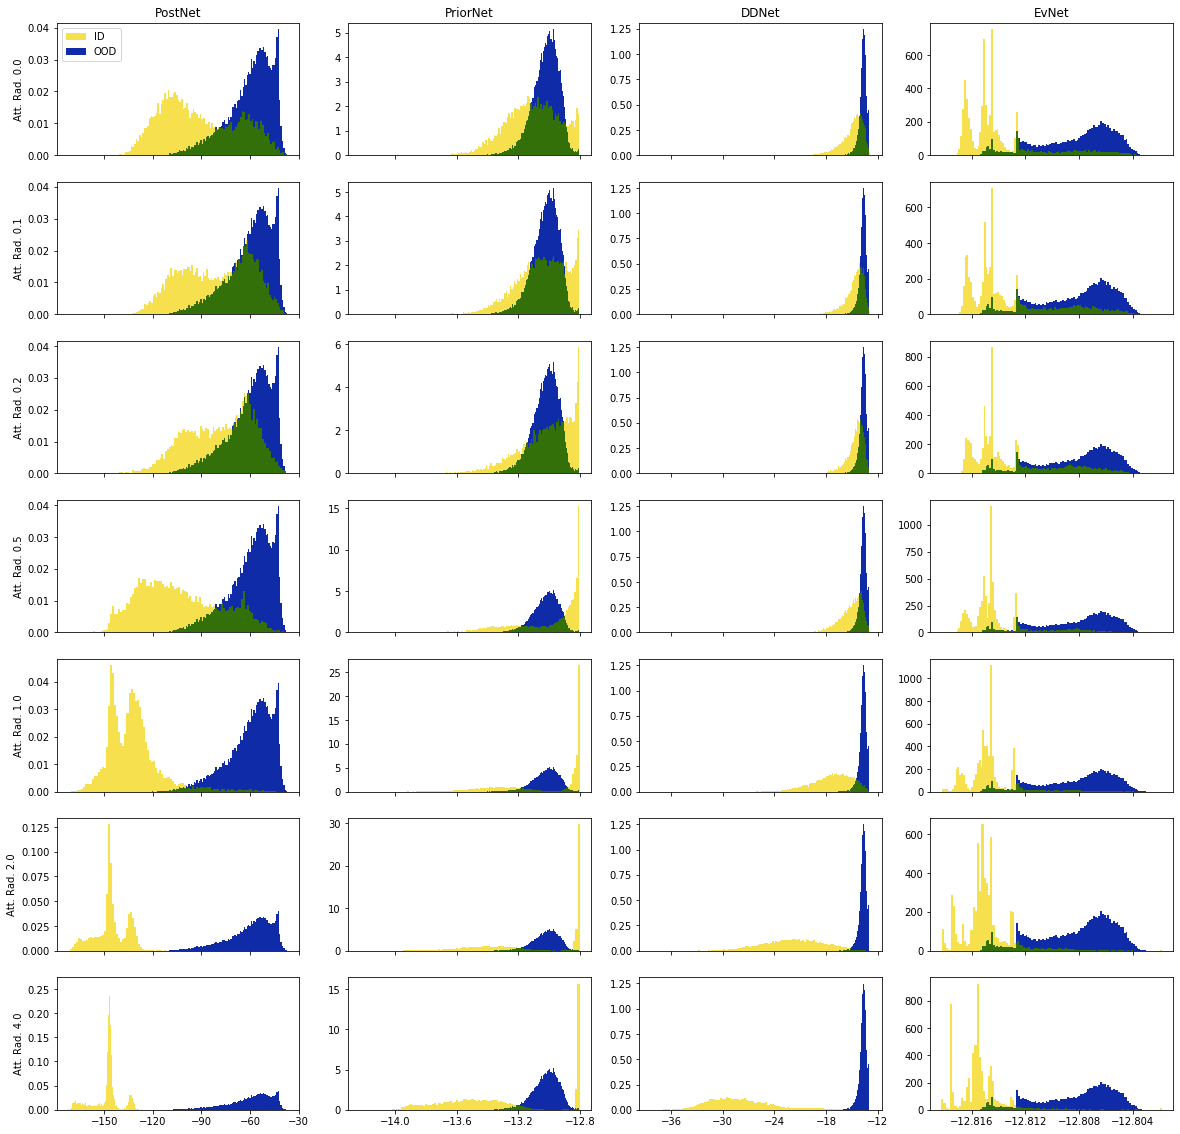
\includegraphics[width=0.99 \textwidth]{sections/008_icml2021/eval/unc_dist_label_id_cifar10_c.png}
    \end{subfigure}%
    \caption{Visualization of the differential entropy distribution of ID data (CIFAR10) and OOD data (SVHN) under label attack. The first row corresponds to no attack. The other rows correspond do increasingly stronger attack strength.}
    \label{fig:attaked_samples_idood_label_attacks_2}
	\vspace{-.5cm}
\end{figure*}
\newpage

\begin{figure*}[ht!]
    \centering
        \begin{subfigure}[t]{1.0\textwidth}
        \centering
        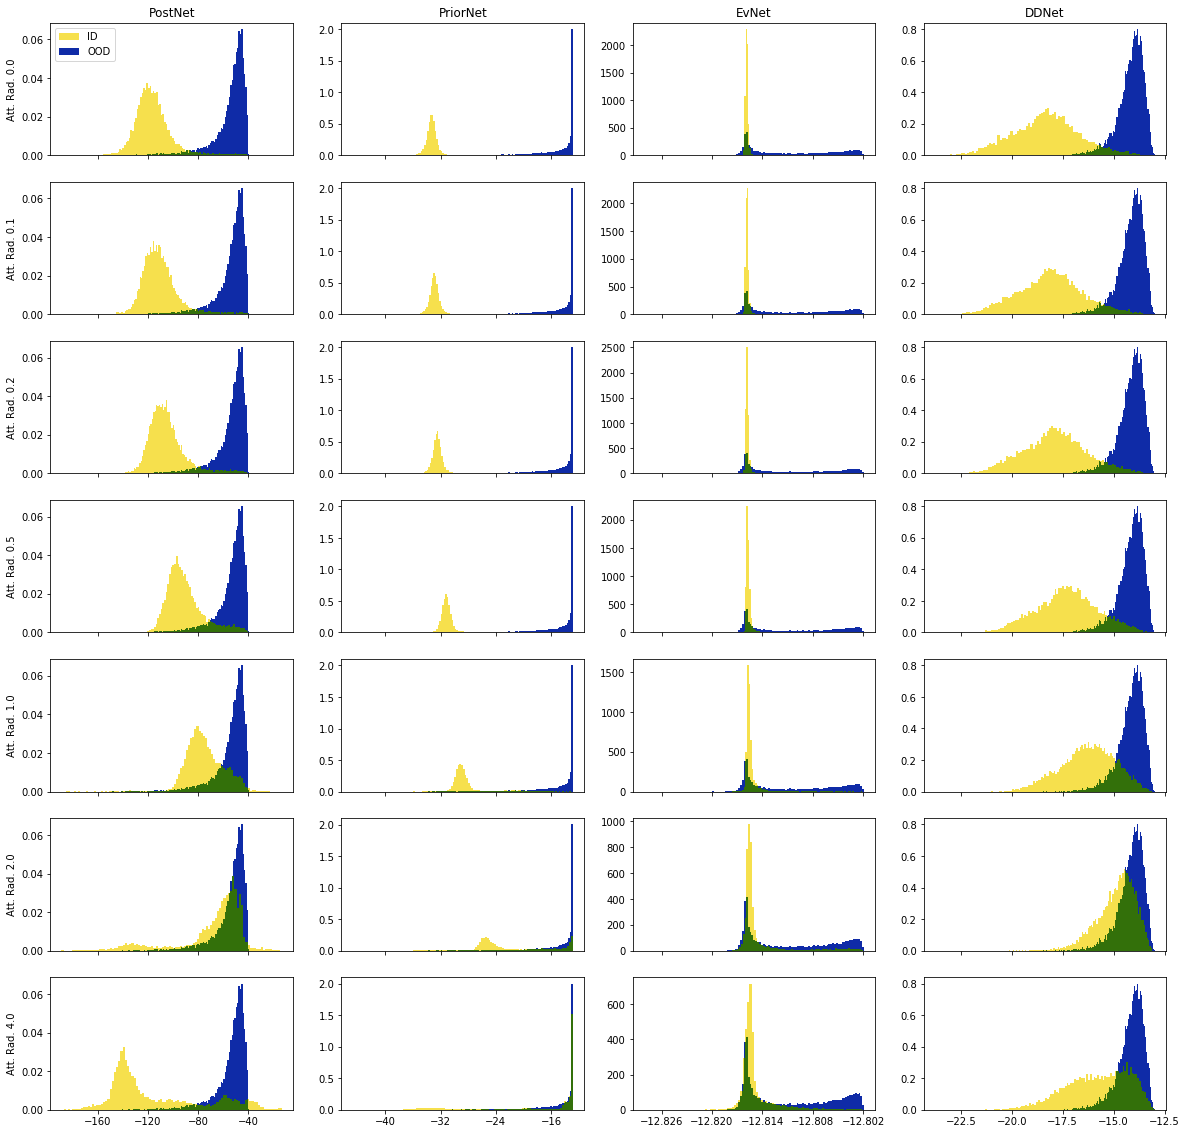
\includegraphics[width=0.99 \textwidth]{sections/008_icml2021/eval/unc_dist_label_id_mnist_c.png}
    \end{subfigure}%
    \caption{Visualization of the differential entropy distribution of ID data (MNIST) and OOD data (KMNIST) under label attack. The first row corresponds to no attack. The other rows correspond do increasingly stronger attack strength.}
    \label{fig:attaked_samples_idood_label_attacks_3}
	\vspace{-.5cm}
\end{figure*}
\newpage

\begin{figure*}[ht!]
    \centering
        \begin{subfigure}[t]{1.0\textwidth}
        \centering
        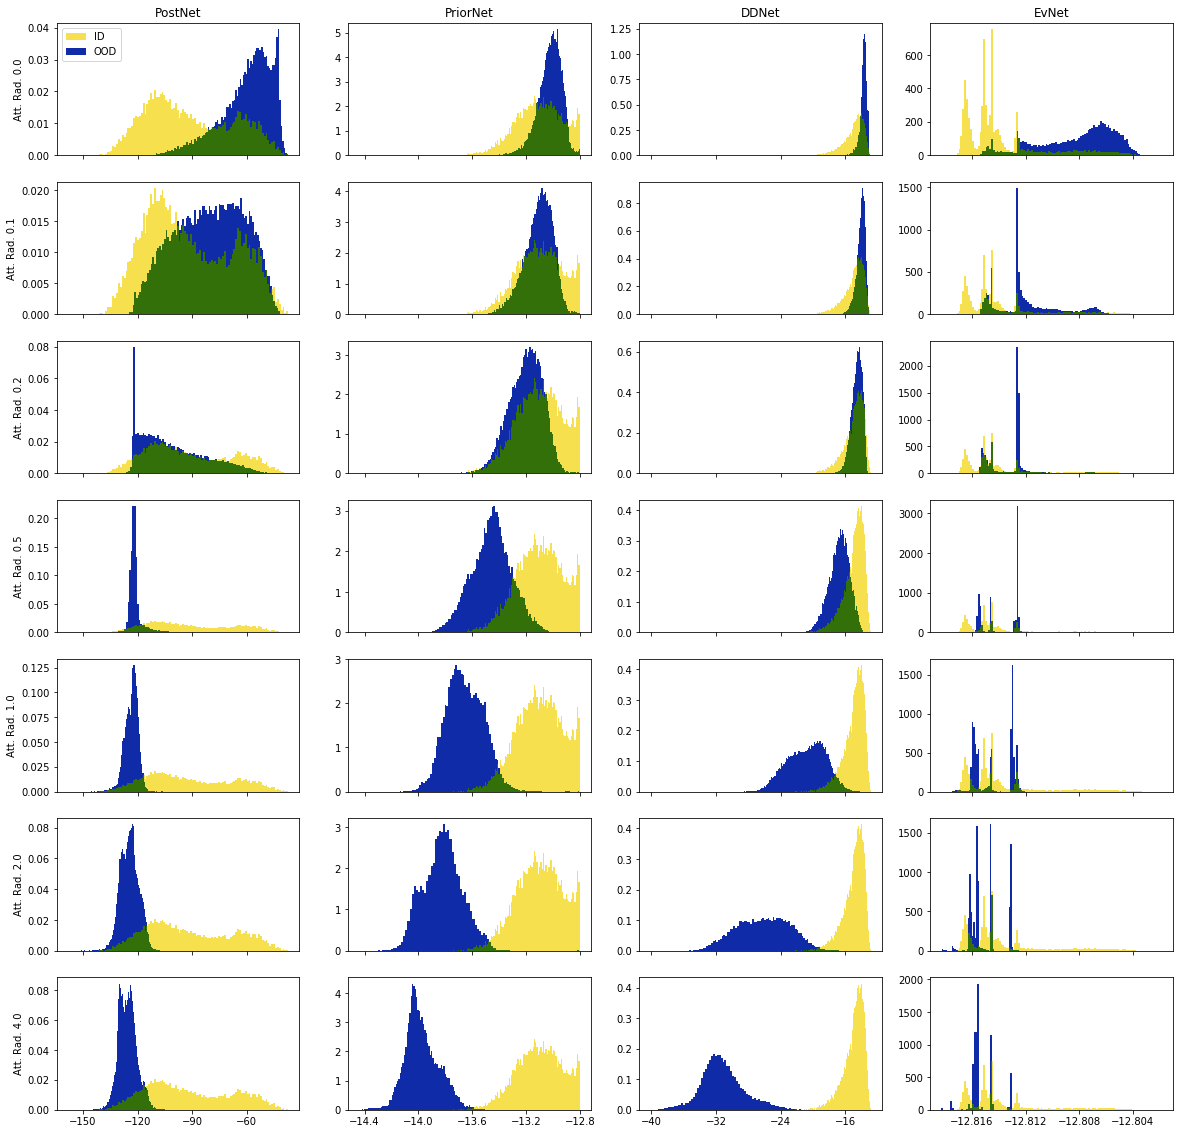
\includegraphics[width=0.99 \textwidth]{sections/008_icml2021/eval/unc_dist_unc_ood_cifar10_c.png}
    \end{subfigure}%
    \caption{Visualization of the differential entropy distribution of ID data (CIFAR10) and OOD data (SVHN) under OOD uncertainty attack. The first row corresponds to no attack. The other rows correspond do increasingly stronger attack strength.}
    \label{fig:attaked_samples_idood_2}
	\vspace{-.5cm}
\end{figure*}


\begin{figure*}[ht!]
    \centering
        \begin{subfigure}[t]{1.0\textwidth}
        \centering
        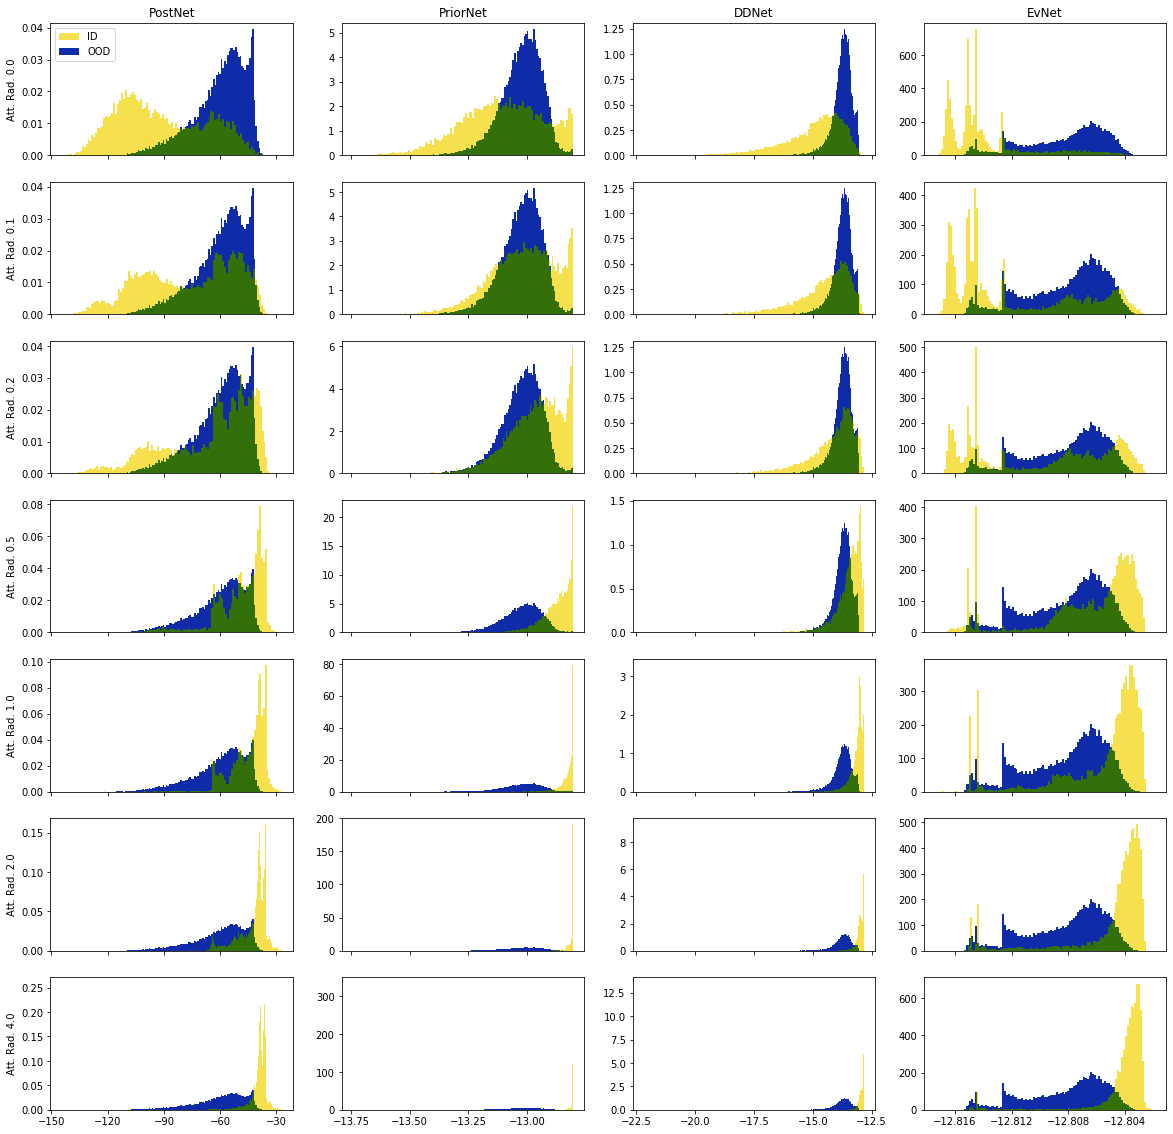
\includegraphics[width=0.99 \textwidth]{sections/008_icml2021/eval/unc_dist_unc_id_cifar10_c.png}
    \end{subfigure}%
    \caption{Visualization of the differential entropy distribution of ID data (CIFAR10) and OOD data (SVHN) under ID uncertainty attack. The first row corresponds to no attack. The other rows correspond do increasingly stronger attack strength.}
    \label{fig:attaked_samples_idood_3}
	\vspace{-.5cm}
\end{figure*}

\begin{figure*}[ht!]
    \centering
        \begin{subfigure}[t]{1.0\textwidth}
        \centering
        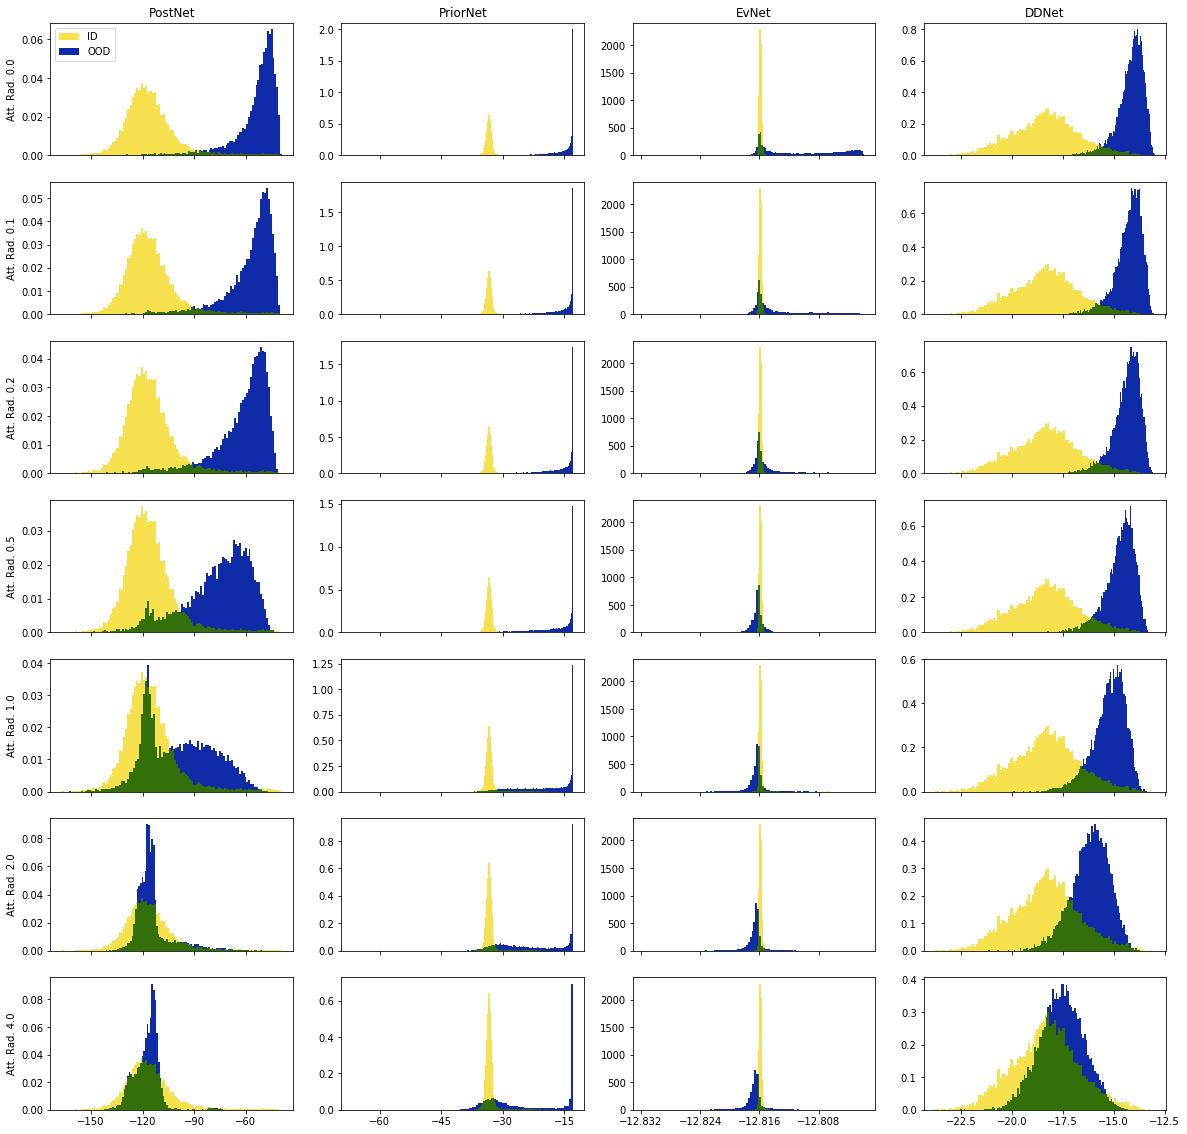
\includegraphics[width=0.99 \textwidth]{sections/008_icml2021/eval/unc_dist_unc_ood_mnist_c.png}
    \end{subfigure}%
    \caption{Visualization of the differential entropy distribution of ID data (MNIST) and OOD data (KMNIST) under OOD uncertainty attack. The first row corresponds to no attack. The other rows correspond do increasingly stronger attack strength.}
    \label{fig:attaked_samples_idood_mnist}
	\vspace{-.5cm}
\end{figure*}


\begin{figure*}[ht!]
    \centering
        \begin{subfigure}[t]{1.0\textwidth}
        \centering
        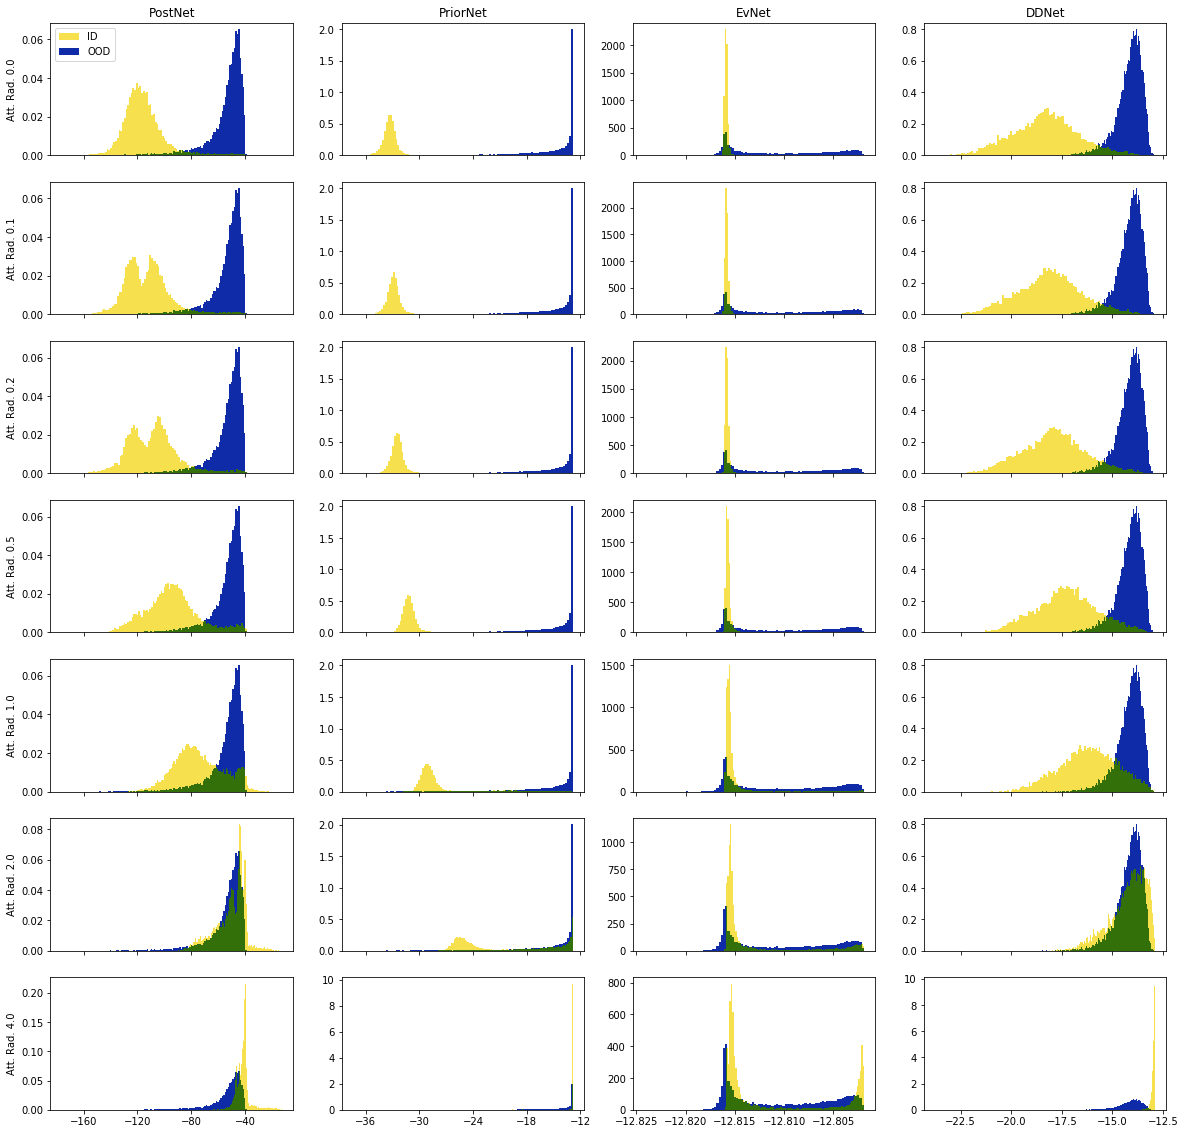
\includegraphics[width=0.99 \textwidth]{sections/008_icml2021/eval/unc_dist_unc_id_mnist_c.png}
    \end{subfigure}%
    \caption{Visualization of the differential entropy distribution of ID data (MNIST) and OOD data (KMNIST) under ID uncertainty attack. The first row corresponds to no attack. The other rows correspond do increasingly stronger attack strength.}
    \label{fig:attaked_samples_idood_mnist_2}
	\vspace{-.5cm}
\end{figure*}






